%==============================================================================
% Tento soubor použijte jako základ
% This file should be used as a base for the thesis
% Autoři / Authors: 2008 Michal Bidlo, 2022 Jaroslav Dytrych
% Kontakt pro dotazy a připomínky: sablona@fit.vutbr.cz
% Contact for questions and comments: sablona@fit.vutbr.cz
%==============================================================================
% kódování: UTF-8 (zmena prikazem iconv, recode nebo cstocs)
% encoding: UTF-8 (you can change it by command iconv, recode or cstocs)
%------------------------------------------------------------------------------
% zpracování / processing: make, make pdf, make clean
%==============================================================================
% Soubory, které je nutné upravit nebo smazat: / Files which have to be edited or deleted:
%   projekt-20-literatura-bibliography.bib - literatura / bibliography
%   projekt-01-kapitoly-chapters.tex - obsah práce / the thesis content
%   projekt-01-kapitoly-chapters-en.tex - obsah práce v angličtině / the thesis content in English
%   projekt-30-prilohy-appendices.tex - přílohy / appendices
%   projekt-30-prilohy-appendices-en.tex - přílohy v angličtině / appendices in English
%==============================================================================
\documentclass[]{fitthesis} % bez zadání - pro začátek práce, aby nebyl problém s překladem
%\documentclass[english]{fitthesis} % without assignment - for the work start to avoid compilation problem
%\documentclass[zadani]{fitthesis} % odevzdani do IS VUT a/nebo tisk s barevnými odkazy - odkazy jsou barevné
%\documentclass[english,zadani]{fitthesis} % for submission to the IS VUT and/or print with color links - links are color
%\documentclass[zadani,print]{fitthesis} % pro černobílý tisk - odkazy jsou černé
%\documentclass[english,zadani,print]{fitthesis} % for the black and white print - links are black
%\documentclass[zadani,cprint]{fitthesis} % pro barevný tisk - odkazy jsou černé, znak VUT barevný
%\documentclass[english,zadani,cprint]{fitthesis} % for the print - links are black, logo is color
% * Je-li práce psaná v anglickém jazyce, je zapotřebí u třídy použít 
%   parametr english následovně:
%   If thesis is written in English, it is necessary to use 
%   parameter english as follows:
%      \documentclass[english]{fitthesis}
% * Je-li práce psaná ve slovenském jazyce, je zapotřebí u třídy použít 
%   parametr slovak následovně:
%   If the work is written in the Slovak language, it is necessary 
%   to use parameter slovak as follows:
%      \documentclass[slovak]{fitthesis}
% * Je-li práce psaná v anglickém jazyce se slovenským abstraktem apod., 
%   je zapotřebí u třídy použít parametry english a enslovak následovně:
%   If the work is written in English with the Slovak abstract, etc., 
%   it is necessary to use parameters english and enslovak as follows:
%      \documentclass[english,enslovak]{fitthesis}

% Základní balíčky jsou dole v souboru šablony fitthesis.cls
% Basic packages are at the bottom of template file fitthesis.cls
% zde můžeme vložit vlastní balíčky / you can place own packages here


% Pro seznam zkratek lze využít balíček Glossaries - nutno odkomentovat i níže a při kompilaci z konzoly i v Makefile (plnou verzi pro Perl, nebo lite)
% The Glossaries package can be used for the list of abbreviations - it is necessary to uncomment also below. When compiling from the console also in the Makefile (full version for Perl or lite)
%\usepackage{glossaries}
%\usepackage{glossary-superragged}
%\makeglossaries 

% Nastavení cesty k obrázkům
% Setting of a path to the pictures
%\graphicspath{{obrazky-figures/}{./obrazky-figures/}}
%\graphicspath{{obrazky-figures/}{../obrazky-figures/}}

%---rm---------------
\renewcommand{\rmdefault}{lmr}%zavede Latin Modern Roman jako rm / set Latin Modern Roman as rm
%---sf---------------
\renewcommand{\sfdefault}{qhv}%zavede TeX Gyre Heros jako sf
%---tt------------
\renewcommand{\ttdefault}{lmtt}% zavede Latin Modern tt jako tt

% vypne funkci šablony, která automaticky nahrazuje uvozovky,
% aby nebyly prováděny nevhodné náhrady v popisech API apod.
% disables function of the template which replaces quotation marks
% to avoid unnecessary replacements in the API descriptions etc.
\csdoublequotesoff

\usepackage{url}

% =======================================================================
% balíček "hyperref" vytváří klikací odkazy v pdf, pokud tedy použijeme pdflatex
% problém je, že balíček hyperref musí být uveden jako poslední, takže nemůže
% být v šabloně
% "hyperref" package create clickable links in pdf if you are using pdflatex.
% Problem is that this package have to be introduced as the last one so it 
% can not be placed in the template file.
\ifWis
\ifx\pdfoutput\undefined % nejedeme pod pdflatexem / we are not using pdflatex
\else
  \usepackage{color}
  \usepackage[unicode,colorlinks,hyperindex,plainpages=false,pdftex]{hyperref}
  \definecolor{hrcolor-ref}{RGB}{223,52,30}
  \definecolor{hrcolor-cite}{HTML}{2F8F00}
  \definecolor{hrcolor-urls}{HTML}{092EAB}
  \hypersetup{
	linkcolor=hrcolor-ref,
	citecolor=hrcolor-cite,
	filecolor=magenta,
	urlcolor=hrcolor-urls
  }
  \def\pdfBorderAttrs{/Border [0 0 0] }  % bez okrajů kolem odkazů / without margins around links
  \pdfcompresslevel=9
\fi
\else % pro tisk budou odkazy, na které se dá klikat, černé / for the print clickable links will be black
\ifx\pdfoutput\undefined % nejedeme pod pdflatexem / we are not using pdflatex
\else
  \usepackage{color}
  \usepackage[unicode,colorlinks,hyperindex,plainpages=false,pdftex,urlcolor=black,linkcolor=black,citecolor=black]{hyperref}
  \definecolor{links}{rgb}{0,0,0}
  \definecolor{anchors}{rgb}{0,0,0}
  \def\AnchorColor{anchors}
  \def\LinkColor{links}
  \def\pdfBorderAttrs{/Border [0 0 0] } % bez okrajů kolem odkazů / without margins around links
  \pdfcompresslevel=9
\fi
\fi
% Řešení problému, kdy klikací odkazy na obrázky vedou za obrázek
% This solves the problems with links which leads after the picture
\usepackage[all]{hypcap}


% Informace o práci/projektu / Information about the thesis
%---------------------------------------------------------------------------
\projectinfo{
  %Prace / Thesis
  project={BP},            %typ práce BP/SP/DP/DR  / thesis type (SP = term project)
  year={2025},             % rok odevzdání / year of submission
  date=\today,             % datum odevzdání / submission date
  %Nazev prace / thesis title
  title.cs={Digitální záznamová jednotka se záznamem dat na paměťové médium s prevencí ztráty dat při výpadku napájení},  % název práce v češtině či slovenštině (dle zadání) / thesis title in czech language (according to assignment)
  title.en={Thesis title}, % název práce v angličtině / thesis title in english
  %title.length={14.5cm}, % nastavení délky bloku s titulkem pro úpravu zalomení řádku (lze definovat zde nebo níže) / setting the length of a block with a thesis title for adjusting a line break (can be defined here or below)
  %sectitle.length={14.5cm}, % nastavení délky bloku s druhým titulkem pro úpravu zalomení řádku (lze definovat zde nebo níže) / setting the length of a block with a second thesis title for adjusting a line break (can be defined here or below)
  %dectitle.length={14.5cm}, % nastavení délky bloku s titulkem nad prohlášením pro úpravu zalomení řádku (lze definovat zde nebo níže) / setting the length of a block with a thesis title above declaration for adjusting a line break (can be defined here or below)
  %Autor / Author
  author.name={Tomáš},   % jméno autora / author name
  author.surname={Dolák},   % příjmení autora / author surname 
  %author.title.p={Bc.}, % titul před jménem (nepovinné) / title before the name (optional)
  %author.title.a={Ph.D.}, % titul za jménem (nepovinné) / title after the name (optional)
  %Ustav / Department
  department={UPSY}, % doplňte příslušnou zkratku dle ústavu na zadání: UPSY/UIFS/UITS/UPGM / fill in appropriate abbreviation of the department according to assignment: UPSY/UIFS/UITS/UPGM
  % Školitel / supervisor
  supervisor.name={Václav},   % jméno školitele / supervisor name 
  supervisor.surname={Šímek},   % příjmení školitele / supervisor surname
  supervisor.title.p={Ing.},   %titul před jménem (nepovinné) / title before the name (optional)
  supervisor.title.a={},    %titul za jménem (nepovinné) / title after the name (optional)
  % Klíčová slova / keywords
  keywords.cs={Sem budou zapsána jednotlivá klíčová slova v českém (slovenském) jazyce, oddělená čárkami.}, % klíčová slova v českém či slovenském jazyce / keywords in czech or slovak language
  keywords.en={Sem budou zapsána jednotlivá klíčová slova v anglickém jazyce, oddělená čárkami.}, % klíčová slova v anglickém jazyce / keywords in english
  %keywords.en={Here, individual keywords separated by commas will be written in English.},
  % Abstrakt / Abstract
  abstract.cs={Do tohoto odstavce bude zapsán výtah (abstrakt) práce v českém (slovenském) jazyce.}, % abstrakt v českém či slovenském jazyce / abstract in czech or slovak language
  abstract.en={Do tohoto odstavce bude zapsán výtah (abstrakt) práce v anglickém jazyce.}, % abstrakt v anglickém jazyce / abstract in english
  %abstract.en={An abstract of the work in English will be written in this paragraph.},
  % Prohlášení (u anglicky psané práce anglicky, u slovensky psané práce slovensky; u projektové praxe lze zakomentovat) / Declaration (for thesis in english should be in english; for project practice can be commented out)
  declaration={Prohlašuji, že jsem tuto bakalářskou práci vypracoval samostatně pod vedením pana X...
Další informace mi poskytli...
Uvedl jsem všechny literární prameny, publikace a další zdroje, ze kterých jsem čerpal.},
  %declaration={I hereby declare that this Bachelor's thesis was prepared as an original work by the author under the supervision of Mr. X
% The supplementary information was provided by Mr. Y
% I have listed all the literary sources, publications and other sources, which were used during the preparation of this thesis.},
  % Poděkování (nepovinné, nejlépe v jazyce práce; nechcete-li, zakomentujte pro skrytí nadpisu) / Acknowledgement (optional, ideally in the language of the thesis; comment out for hiding including heading)
  acknowledgment={V této sekci je možno uvést poděkování vedoucímu práce a těm, kteří poskytli odbornou pomoc
(externí zadavatel, konzultant apod.).},
  %acknowledgment={Here it is possible to express thanks to the supervisor and to the people which provided professional help
%(external submitter, consultant, etc.).},
  % Rozšířený abstrakt (cca 3 normostrany) - lze definovat zde nebo níže / Extended abstract (approximately 3 standard pages) - can be defined here or below
  %extendedabstract={Do tohoto odstavce bude zapsán rozšířený výtah (abstrakt) práce v českém (slovenském) jazyce.},
  %extabstract.odd={true}, % Začít rozšířený abstrakt na liché stránce? / Should extended abstract start on the odd page?
  %faculty={FIT}, % FIT/FEKT/FSI/FA/FCH/FP/FAST/FAVU/USI/DEF
  faculty.cs={Fakulta informačních technologií}, % Fakulta v češtině - pro využití této položky výše zvolte fakultu DEF / Faculty in Czech - for use of this entry select DEF above
  faculty.en={Faculty of Information Technology}, % Fakulta v angličtině - pro využití této položky výše zvolte fakultu DEF / Faculty in English - for use of this entry select DEF above
  department.cs={Ústav počítačových systémů}, % Ústav v češtině - pro využití této položky výše zvolte ústav DEF nebo jej zakomentujte / Department in Czech - for use of this entry select DEF above or comment it out
  department.en={Department of Computer Systems} % Ústav v angličtině - pro využití této položky výše zvolte ústav DEF nebo jej zakomentujte / Department in English - for use of this entry select DEF above or comment it out
}

% Rozšířený abstrakt (cca 3 normostrany) - lze definovat zde nebo výše / Extended abstract (approximately 3 standard pages) - can be defined here or above
%\extendedabstract{Do tohoto odstavce bude zapsán výtah (abstrakt) práce v českém (slovenském) jazyce.}
% Začít rozšířený abstrakt na liché stránce? / Should extended abstract start on the odd page?
%\extabstractodd{true}

% nastavení délky bloku s titulkem pro úpravu zalomení řádku - lze definovat zde nebo výše / setting the length of a block with a thesis title for adjusting a line break - can be defined here or above
%\titlelength{14.5cm}
% nastavení délky bloku s druhým titulkem pro úpravu zalomení řádku - lze definovat zde nebo výše / setting the length of a block with a second thesis title for adjusting a line break - can be defined here or above
%\sectitlelength{14.5cm}
% nastavení délky bloku s titulkem nad prohlášením pro úpravu zalomení řádku - lze definovat zde nebo výše / setting the length of a block with a thesis title above declaration for adjusting a line break - can be defined here or above
%\dectitlelength{14.5cm}

% řeší první/poslední řádek odstavce na předchozí/následující stránce
% solves first/last row of the paragraph on the previous/next page
\clubpenalty=10000
\widowpenalty=10000

% checklist
\newlist{checklist}{itemize}{1}
\setlist[checklist]{label=$\square$}

% Kompilace po částech (rychlejší, ale v náhledu nemusí být vše aktuální)
% Compilation piecewise (faster, but not all parts in preview will be up-to-date)
% Další informace viz / For more information see https://www.overleaf.com/learn/latex/Multi-file_LaTeX_projects
% \usepackage{subfiles}

% Nechcete-li, aby se u oboustranného tisku roztahovaly mezery pro zaplnění stránky, odkomentujte následující řádek / If you do not want enlarged spacing for filling of the pages in case of duplex printing, uncomment the following line
% \raggedbottom

\begin{document}
  % Vysazeni titulnich stran / Typesetting of the title pages
  % ----------------------------------------------
  \maketitle
  % Obsah
  % ----------------------------------------------
  \setlength{\parskip}{0pt}

  {\hypersetup{hidelinks}\tableofcontents}
  
  % Seznam obrazku a tabulek (pokud prace obsahuje velke mnozstvi obrazku, tak se to hodi)
  % List of figures and list of tables (if the thesis contains a lot of pictures, it is good)
  \ifczech
    \renewcommand\listfigurename{Seznam obrázků}
  \fi
  \ifslovak
    \renewcommand\listfigurename{Zoznam obrázkov}
  \fi
  {\hypersetup{hidelinks}\listoffigures}
  
  \ifczech
    \renewcommand\listtablename{Seznam tabulek}
  \fi
  \ifslovak
    \renewcommand\listtablename{Zoznam tabuliek}
  \fi
  % {\hypersetup{hidelinks}\listoftables}

  % Seznam zkratek / List of abbreviations
  %\ifczech
  %  \renewcommand*\glossaryname{Seznam zkratek}%
  %  \renewcommand*\entryname{Zkratka}
  %  \renewcommand*\descriptionname{Význam}
  %\fi
  %\ifslovak
  %  \renewcommand*\glossaryname{Zoznam skratiek}%
  %  \renewcommand*\entryname{Skratka}
  %  \renewcommand*\descriptionname{Význam}
  %\fi
  %\ifenglish
  %  \renewcommand*\glossaryname{List of abbreviations}%
  %  \renewcommand*\entryname{Abbreviation}
  %  \renewcommand*\descriptionname{Meaning}
  %\fi
  % Definice zkratek - z textu se odkazují např. \Gls{TF–IDF}
  % Definition of abbreviations - referred from the text e.g. \Gls{TF–IDF}
  %\newglossaryentry{TF–IDF}
  %{
  %  name={TF–IDF},
  %  description={Term Frequency-Inverse Document Frequency}
  %}
  % 
  %\setglossarystyle{superragged}
  %\printglossaries


  \ifODSAZ
    \setlength{\parskip}{0.5\bigskipamount}
  \else
    \setlength{\parskip}{0pt}
  \fi

  % vynechani stranky v oboustrannem rezimu
  % Skip the page in the two-sided mode
  \iftwoside
    \cleardoublepage
  \fi

  % Text prace / Thesis text
  % ----------------------------------------------
  \ifenglish
    % This file should be replaced with your file with thesis content.
%=========================================================================
% Authors: Michal Bidlo, Bohuslav Křena, Jaroslav Dytrych, Petr Veigend and Adam Herout 2019

% For compilation piecewise (see projekt.tex), it is necessary to uncomment it and change
% \documentclass[../projekt.tex]{subfiles}
% \begin{document}

\chapter{Introduction}

This text serves as an example content of this template and as a recap of the most important information from regulations, it also provides additional useful information, that you will need when you write a technical report for your academic work. Check out appendix \ref{jak} before you use this template as it contains vital information on how to use it.

Even though some students only need to know and comply with the official formal requirements stated in regulations as well as typographical principles to write a good diploma thesis (a bachelor's thesis is a diploma thesis too -- you get a diploma for it), it is never a~bad idea to familiarize yourself with some of the well-established procedures for writing a~technical text and make things easier for yourself. Some supervisors had prepared breakdowns of proven procedures that have led to tens of successfully presented academic works. A~selection of the most interesting procedures available to the authors of this work at the time of writing can be found in the chapters below. If your supervisor has their own web page with recommended procedures, you can skip these chapters and follow their instructions instead. If that is not the case, you should read the respective chapters prior to consulting your supervisor about the structure and contents of your academic work.

Diploma thesis is an extensive work and the technical report should reflect it. It is not easy for everyone to sit down and simply write it. You need to know where to begin and how to progress. One of many viable approaches is to start with keywords and abstract, this helps you establish what the most important part of your work is. More on that in~chapter~\ref{abstrakt}.

Once the abstract is finished, you can start with the text of the technical report. The first thing you should do is create a structure for your work, that you'll later fill with text. Chapter \ref{struktura} provides basic information and hints on writing a technical text, that can help you avoid mistakes beginners make, create chapter titles, and figure out what the approximate length of individual chapters should be. The chapter concludes with an approach that should make writing a thesis much easier.

Diploma theses in the field of information technology have a specific structure. The introduction is followed by a chapter or chapters dealing with the summary of the current state. The next chapter should evaluate the current state and provide a solution, that will be implemented and tested. The conclusion should contain evaluated results and ideas for future development. Even though the chapter titles and their length may differ from other theses, you can always find chapters that correspond with this structure. Chapter \ref{kapitoly} deals with the contents of chapters that commonly occur in diploma theses in the field of information technology. Most students will only use a subset of all the described chapters as not everything will be relevant to their thesis. The descriptions and hints provided help students with the inner structure and the contents of chapters as well as decide whether or not they should even include a given chapter. 

The final chapter of a thesis is always followed by a list of references. Citations that this list is comprised of and their respective links are the subject of chapter \ref{citace}. An inexperienced student may not perceive it that way, but the list of references is a vital part of a thesis. One of the important aspects of your reviewer's evaluation is how you work with literature. A single missing entry can lead to an F for your grade, disciplinary proceedings for plagiarism, and ultimately to being expelled. There are other consequences to this as two Czech ministers resigned over allegations of plagiarism in 2018. Be as thorough as possible in creating your list of references.

When you're done with the text, it is necessary to figure out what the requirements for a thesis at BUT FIT are and work the kinks out. Formal requirements that are stated in~regulations and on faculty web pages can be found in chapter \ref{formality}. This chapter also contains information about the required length of different types of academic works and other helpful information. The chapter concludes with an overview of the most common mistakes that the reviewers have to deal with and that you should avoid. The review of the formal aspect of the thesis is just another important part of the reviewer's assessment.

Once you deal with the formal deficiencies, you can submit your thesis. Before you do so, go through the checklist in appendix \ref{checklist}. The submission of paper and electronic versions of a thesis is described in chapter \ref{odevzdani}.

Chapter \ref{zaver} contains a summary of what you can learn by reading this text, and most importantly things to keep in mind before you submit your thesis.

\chapter{Abstract}
\label{abstrakt}

There should be a summary of work at most 10 lines long under the Abstract heading. Despite how short it is, a good abstract provides enough information to know what the problem is, what was the chosen solution as well as the results achieved. The purpose of an abstract is to let the reader know whether or not they can find the answer to their question here. The rest of this chapter was taken from professor Herout's blog \cite{Herout}.
\bigskip

\noindent First and foremost - abstract matters. Second - It's not that hard to write one. Without further ado, let's dive into it.

\subsection*{What is the purpose of an abstract}
An abstract is used for \bf searching \rm purposes, together with the title of the thesis and a list of keywords. These parts (perhaps except for the title) are not directly part of the text and it's not expected that anyone who will read your thesis actually reads them. The fact that they're reading your thesis means they're past the abstract stage. Abstract serves them well to decide \bf whether or not \rm they want to read your thesis.

When someone looks for an answer to their problem, they give the librarian or a search engine (these days) keywords that directly relate to their problem. They then receive a list of theses, that could possibly offer a solution based on the match between the keywords used and keywords in the theses. A good thesis title can help the person guess which texts could have a direct relation to their problem and can get them to read your thesis.

This is where the abstract is crucial. The reader reads abstracts of the theses and decides, whether or not they want to read them. It also informs them that their filter based on a title alone is wrong.

At this point, they don't have a PDF with full text or a printed version of the thesis available. Abstracts are \bf not \rm supposed to be in the text itself, but to be available on servers aggregating scientific texts. Therefore the first rule is: an abstract needs to work on its own -- if it contains references to literature or text (``The efficiency of a method is summarized on page 51.''), it only makes a reader less interested in the author, won't read their work or cite them.


\subsection*{When and how to write an abstract}
It makes sense to write an abstract when the writing is done -- as a summary and real annotation of the thesis.
I however like the opposite approach -- write an abstract in the beginning. Whenever I write a scientific article, I start with a long list of keywords that are related to each other. It's a lot more than end up as the final keywords used for indexing. It helps me understand where the article is headed at all times -- what should I talk about, what needs to be in the text, what does it deal with? As soon as I'm done with keywords, I form a title and an abstract.

I consider the following four parts of an abstract especially useful -- Which problem does it solve? What solution does it offer? What are the results? What is the meaning of these results? Once all of this is clear, the text essentially writes itself. If this is unclear, how on earth can you form a coherent, meaningful sentence in the same text?


\subsection*{Recommended structure of the abstract}
An abstract of a scientific thesis can consist of four parts and be useful. Each part consists of two to three sentences, in some cases even a single sentence is enough.

The term ``elevator pitch'' is often used in business. It is not a coincidence that its structure is similar to the recommended structure of an abstract. Realistically, an abstract should contain anything the author would say about their scientific thesis if they had at most 2 minutes and could not use slides, images, or text. What should they talk about then?

\paragraph{Part one -- What is the problem? What is the topic? What's the goal of the text?}
\begin{itemize}
  \item{This thesis deals with.}
  \item{The goal of this thesis is.}
  \item{My aim was.}
\end{itemize}
There is no place for fairy tales specific to wrong scientific literature: ``Our five-year-plan of~work open new and bold goals for us'', ``With the evolution of computing technology and especially the display devices, it is more important than ever \ldots'' do not belong anywhere near a good text, especially an abstract. If you can express the purpose of your text in one sentence, do it and forget about everything else. Less is always more when it comes to the abstract.

\paragraph{Part two -- How is the problem solved? Is the goal fulfilled?}
\begin{itemize}
  \item{I solved the problem using this and that.}
  \item{I used this method, this procedure and analyzed this.}
  \item{The work represents an algorithm that.}
  \item{I used these tools to process data and evaluated results like this.}
  \item{The principle of our algorithm is.}
\end{itemize}

There is a new methodology in the nature of scientific text (= ``how to do something''), it needs to include a description. If the solution consists of three parts, it probably means that this part of an abstract will have three sentences, where each sentence is about a~different part of the solution. A good abstract should be honest and accurate in this section -- no ``revealing secrets'' in the text itself. Vague formulations of a solution principle in~an~abstract usually means that the authors can't write or don't have anything to write about -- neither one is good enough to waste your time.

\paragraph{Part three -- What are the results? How good is the solution?}
\begin{itemize}
  \item{It was 87,3\,\% successful.}
  \item{We created a system that.}
  \item{The solution offers these options.}
  \item{As a result, we found out that.}
\end{itemize}

Stating a specific number is not a bad habit in this part -- ``we made existing XY method five times faster''. If the contribution of your work cannot be summarized in two or three sentences, something is wrong and the entire text is probably not worth writing.

\paragraph{Part four -- Well then? What does it bring to science and the reader?}
\begin{itemize}
  \item{The contribution of this thesis is.}
  \item{The primary discovery is.}
  \item{The primary result is.}
  \item{Based on the data it is possible to.}
  \item{The results allow us to.}
\end{itemize}

When writing scientific articles, I myself struggle with the similarity of third and fourth part. Both of them speak about the results and contribution of the text. The goal of the third part is to be specific and name achieved results whereas the goal of the fourth part is to interpret their meaning and significance. I guess it's fine if these two statements merge to an extent and both parts not only don't have their own paragraph, but they sometimes even intertwine with their common sentences.

\paragraph{Part zero -- What is it about? Where are we?}
\begin{itemize}
  \item{The context is this and this.}
  \item{It deals with studies of this and that.}
  \item{We build on these recent advances in our field.}
\end{itemize}

Sometimes it is necessary to insert a short specification of context at the beginning of your abstract. It can be a great asset when it comes to obscure and esoteric field, that is off to the side of the main flow. Usually, this part is not needed and sentences contained here are prime examples of pseudoscientific nonsense. It's not necessarily bad to forget that this part can even exist in an abstract. If an expert in the field shakes their head after reading an abstract: ``I have no idea what this is about.'' only then it makes sense to include this part to specify context.


\subsection*{Innovation is not ignorance}

In this text, I describe a general model of a general thesis. I would like to state that this is my opinion and taste and I'm interested in alternate opinions and tastes (I really am!). Every graduate (Mgr. and Bc.) feels that their thesis is special and extraordinary. Therefore they won't follow some scheme meant for common and average theses -- i.e. the others. I see good reasons to divert from the outlined scheme and recommend some students to divert from the scheme myself every year. Indeed, every thesis is unique and extraordinary. If they weren't, there would be no reason to write them, just copy them instead. Before you divert from the standard and canonical way of organizing scientific text, put some effort into learning, understanding and tackling it. The way of scientific work, structuring scientific text, or citing sources can look rigid and clumsy, but for now it is the best way mankind could come up with. If you learn it, understand its advantages and disadvantages and innovate it, it's great and you're welcome to do so. If you choose to ignore it, you'll most likely end up with a very poor innovation.

\chapter{Drafting the basic thesis structure}
\label{struktura}

This chapter contains a selection of useful hints and procedures useful for writing a dissertation (bachelor's thesis is technically a dissertation -- you receive a diploma for it) from experienced supervisors. First a number of general principles are listed, followed by a more detailed description of the advised procedure of drafting a thesis structure.

Before you into it head first, ask your supervisor for any advice or if they have their own web page with hints and guidelines. Their area of expertise will probably coincide with that of your thesis and help you with the most appropriate structure that you should comply with. If the authors learn about another collection of useful hints, you'll find it here in the future.

This text deals with the general recommendations and thesis structure, which always has to be modified and thought of based on the specification \cite{Cernocky}.


\section{Useful hints for writing a technical text}

The following instructions can also be found on faculty web pages\cite{fitWeb}. The overview of basic typography and the creation of documents using \LaTeX{} system can be found in Jiří Rybička's book\cite{Rybicka}.

One of the evaluated parts of a potential engineer is quality of language and literacy. Your goal is to create a clear and comprehensive text. You should express yourself accurately, use the appropriate level of Czech or Slovak grammar (or English if need be) and comply with the generally accepted customs. Slang words and phrases are not allowed. If you are uncertain of the translation or transcription of foreign terms, use literature available in FIT library.

The text should be a short path to understanding a problem, predict it's difficulties and preventing them. Good writing means perfect grammar, correct punctuation and use of appropriate words. You should strive for a good text, one that is not monotonous due to use of small selection of words, or overuse of some of your favorite words. If you use foreign words, it is expected that you know their exact meaning. Obviously, you need to use english words correctly as well. For example, there are certain rules when using the word {\it obvious}. Is {\it obvious} really obvious? And did you make sure, that the {\it obvious} is really valid? You should be careful about using the subject {\it it} with a passive voice too often. For example, you should never use the Czech {\it it has proved itself that...}, ever.

It is advised to think the use of symbols for {\it labeling} through thoroughly. By this we mean a well-thought-out choice of abbreviations and symbols used for distinguishing types of parts, labeling program's main functions, naming control keys on the keyboard, naming variables in math formulas, etc. Apt and consistent labeling can help readers a lot. It is advised to provide a list of labeling at the beginning of the text. Not just in labeling, consistency is important in references and in typesetting in general.

There are numerous typographical principles that can be used to distinguish things. You can choose different styles for different purposes. As an example, keys can be placed in a rectangle, identifiers from source text can be written in {\tt typewriter font} etc.

Whenever you state facts, you should also state their origin and your attitude to them. If you claim something, you always have to explicitly state, which part of it was proven, what will be proven in your text and what you took from literature (including its source). You should never let the reader doubt whose idea they're presented with, your own or someone else's.


If you want to write a clear and comprehensive academic text, you need to follow these rules:
\begin{itemize}
\item You must have something to say,
\item you must know, who you want to say it to,
\item you must thoroughly think through the contents,
\item you must write in a structured way 
\end{itemize}

\subsection*{You must have something to say}
The most important prerequisite of a good academic text is to have an idea. If the idea is significant enough, it will last, even if it is not formulated in the best way. However, if you want to articulate your idea as precisely as possible and save the reader's time, you must comply with certain principles discussed further below.

\subsection*{You must know, who you want to say it to}
Another important prerequisite of a good academic text is the audience. If you write down notes for yourself, you usually write in a differently than when you write a scientific report, article, thesis, book or a letter. Depending on who the target audience is, you can decide the writing style, the amount of information and how detailed it is. 

\subsection*{You must thoroughly think through the contents}
You must thoroughly think through the contents of your thesis as well as the order in which you want to present the reader with your ideas. As soon as you know what you want to say and to whom, you need to create a structure. The ideal structure should be one that is logically accurate and psychologically digestible, where everything has its place and its individual parts fit into each other. All the connections between them are clear and it's apparently what belongs where.

To achieve this goal, you must precisely structure the contents of your text. Decide what the main chapters and subchapters are going to be, as well as the connection between them. A diagram of such structure would be a tree-like graph, not a chain. When structuring the contents, it is important to ask yourself what you want to include as well as what you want to exclude. Too much detail could discourage the reader, and so could lack of detail.

The result of this stage is an outline of the text consisting of the main ideas and all the details between connecting them to each other.

\subsection*{You must write in a structured way}

You must write in a structured way and work the most comprehensible format simultaneously, with good writing and perfect labelling included. If you have an idea, you know who your target audience is, you know your goal and outline of the text, then you're ready to start writing. When writing your initial draft, you should try to include all your ideas and opinions regarding the individual chapters and subchapters. You need to explain every single idea, describe and prove it. The main idea should always be formulated in a main clause, rather than the dependant clause.

You should approach the writing itself in a structured way too. As you're working on the structure of your thesis, you're creating a framework that you are gradually completing. You should use a DPT\footnote{Desktop publishing (DTP) - creating printed document on a computer.} program that offers a structured layout of the text (pre-defined types of headings and text blocks).

\subsection*{It will never be perfect}
Once you have written everything you thought about, you should take a day or two off, then read what you wrote again. Make the last changes and move on. You should know that something will always remain unfinished and that there is always a better way of explaining something, but every stage of the editing must come to an end.

\section{Who is the target audience of a thesis}

This subsection was taken from professor Herout's blog \cite{Herout}.

\bigskip
\noindent \bf Write your thesis for a student, that will build on your work. \rm
\bigskip

Imagine that another student will continue the work in your thesis, they're about as~smart as you are. You have four hours to show them your thesis, explain everything necessary for them to be able to continue your work. The student studies at the same school and knows about as much as an average student would, they're not an expert in the area of your thesis, but they're not stupid either. The student just found out that they'll continue your work, so they had no time to learn about the topic, just like you.

It's best to start by telling the student what the goal of this thesis is and what the results should look like.

Nobody in their right mind will spend an hour explaining things like this to the student: ``{\mbox{Interet} was invented by the American army in 1962, then www was invented in CERN in 1991, nowadays it is used for various purposes.''}(all of this on six pages with countless references and figures).
The student usually doesn't need countless pages of details regarding colorful modules to represent figures, history and details of Hough transformation, complete description of the ISO/OSI reference model layers or a set of pie graphs representing individual mobile platforms on the market over the last decade.
The student needs to be shown the valuable sources that helped you and wants a brief description of tools and algorithms that were a vital part of the solution: ``{You need XY tool that does this and that, especially it's PQ module, that is used then and then. The most useful information can be found in~this documentation.}''

Tell the student everything about what worked for you and what helped, but also make sure to tell them what seemed like a good idea, but ended up being useless.

Try to provide just the right amount of detail. Explain an optimization method one line of code at a time, a module in one paragraph enriched with description of input and output data, and a reference to the respective library.

Imagine this four hours long session with the student.
\begin{itemize}
  \item{What do you think you would talk about in the beginning, how long did it take for the student to understand?}
  \item{What are some things that should be mentioned?}
  \item{What kind of figures would you draw during the session?}
  \item{What would the student ask about, what is important but not clear?}
  \item{What restrictions and unfinished things would you need to inform the student about to prevent them from falling into a trap?}
  \item{How can the student continue? What is left unfinished and is worth trying? What could be improved?}
  \item{What would you say in the very first and very last minute of the session?}
\end{itemize}


\section{Thesis structure -- Five chapters}

This subsection was taken from the blog of professor Herout\cite{Herout} (partially inspired by a book from Jean-Luc Lebrun \cite{Lebrun2011}) and from a document on professor Zemčík's web page \cite{Zemcik}.
\bigskip

Thesis is something that students work on for 2 semesters of their studies and then write a small book about it. The misconception is that this little book is the master's thesis. The book is in fact a technical report about the year long work and master's thesis represents the result of student's work.

The year long work includes studies first and foremost: ``What already exists in the area of my thesis? How did the others do it?'' It is implied that a student tries to innovate and design some things: ``The problem has several solutions, I chose this approach, because it is the most efficient option for the given platform.''
The researcher should implement and evaluate their designs to validate them: ``I used these tools for implementation, the entire system is split into these modules. The result is this fast, it is this effective and user reviews are such and such.''

The basic structure of master's thesis according to professor Herout is as follows:
\begin{enumerate}
  \item{Introduction (1 page)}
  \item{What had to be studied (including assessment of the current state; 40\,\%)}
  \item{New ideas that this thesis explores (30\,\%)}
  \item{Implementation and evaluation (30\,\%)}
  \item{Conclusion (1 page)}
\end{enumerate}

If the text has these 5 chapters, it is not a mistake, neither is if one of them is split in two parts -- more on that later. A big mistake is when any of the parts are missing, or when it's content differs from the rest.

Names of chapters can vary from this structure, even though your thesis will have an introduction and a conclusion. The content of your thesis itself is what really matters and if it means you have to break the structure, then do so.

Many supervisors agree with this basic structure, even though some of them recommend different chapter titles for example assessment of the current state can be used in the second chapter, and even in the third chapter according to professor Zemčík:
\begin{enumerate}
\item Introduction (1--2 pages)
\item Summary of the current state (40--50\,\%)
\item Assessment of the current state and solution draft (3-5 pages)
\item Your own work (roughly 40\,\%)
\item Conclusion (at most 1 page)
\end{enumerate}

Opinions of supervisors also differ in length depending on the specification of thesis, this can be seen for example in recommendations from assistant professor Beran \cite{Beran}:
\begin{enumerate}
\item Introduction (1 page)
\item Theory (1/3 of pages)
\item Solution draft (1/3 of pages)
\item Implementation, experiments and assessment (1/3 of pages)
\item Conclusion (1 page)
\end{enumerate}

When it comes to practice-oriented theses, where the most important things are data and user interface, associate professor Černocký \cite{Cernocky} recommends the following:
\begin{enumerate}
\item Introduction (single digit of pages)
\item Theoretical part (roughly 10 pages)
\item Data (single digit of pages)
\item Breakdown of Your algorithm and testing (roughly 10 pages)
\item Draft and implementation (several pages)
\item User interface (several pages)
\item Testing (roughly 10 pages)
\item Conclusion (single digit of pages)
\end{enumerate}

\section{Thesis -- comics edition}

This subsection was taken from professor Herout's blog. \cite{Herout}.

Thesis (including bachelor's) is a fairly complex work comprised of a large number of letters. These letters follow a certain hierarchy, organised into chapters. The whole thing should follow a logical order -- reader should first learn one thing so that they can then learn and understand other things. It should contain figures, tables, formulas; these non-textual objects should fit in with the surrounding text and enrich it. Every single aspect of the specification of your thesis has to be explored, it has to be finished by a certain date, printed and bundled into a book. If you want your thesis to be good, you need to make it good. Whenever you bake a cake from ten ingredients and one of them is rotten, it doesn't matter how hard you try, the cake will not taste good.

\subsection*{How should you approach everything?}

Whenever we write an article (all the time lately), we create something called a ``Comics Edition'' in the early stage. We do it because I insist that we do it and because it helps us a lot. Perhaps it can help you with your thesis.

First, make sure you know the answers to the following questions:
\begin{itemize}
  \item{How would you explain the principle of your solution in three to five short sentences?}
  \item{What are the strengths of your solution?}
  \item{What arguments would you use to support the correctness of your solution?}
  \item{If someone wanted to criticize your thesis -- what would they criticize it for?}
  \item{What would your answer be?}
  \item{What keywords should one use in a search engine to find your thesis in the search results?}
\end{itemize}

If you are finished, let's get into it...

\subsection*{Create THE document}

I often see people write an ``initial'' version of a thesis somewhere in their notes. First of all, that's extra work and second it is entirely pointless. It's best to create a document where the fight begins and also ends.

\subsection*{Chapter titles}

Chapter titles are an important part of a comics edition, put them in your document.

Put them in for the sake of formatting -- no provisional bullet point lists: ``I'll just do it later''. You need to see how the automatically generated content looks now, before it's too late to change everything.

Put them in for the sake of wording. Chapter title says, what the chapter is about. Chapter titles represent a skeleton covered in flesh and skin of text and figures.

Of all the words in your thesis, words in the titles are the \textbf most important ones\rm. Put some time and effort into your titles.

\subsection*{Figures}

A picture is worth a thousand words. I went through the last 8 articles that I helped write. They're 80 pages total and contain 87 figures and 17 tables, that's 1,3 of visual information per page (including pages containing references, title pages with abstracts etc). Many figures (about half) are comprised of multiple subfigures, especially referenced figures. I~counted 221 subfigures in the mentioned articles, that's an average of 3 visuals per page. This is what I imagine the role of figures in a scientific text should be. I think a~thesis with ``too many figures'' does not exist.

You should think about what images you will use and where they'll be even in the early stage of comics edition.

Figures don't have to be finished. We don't know what exactly the figure will represent just yet. We don't know what the caption will be. We only know that there will be a figure and that it will be comprised of multiple subfigures. It takes roughly a minute (we already have a vector format of a ``TODO Image'') and it shows us how the text will look.

In some cases, we know what the images will look like on a conceptual level. Draw it on a paper or a blackboard, take a picture of it, and insert it where the final figure will be (vector image made in Inkscape\footnote{\url{https://inkscape.org}} or generated using Gnuplot\footnote{\url{http://www.gnuplot.info/}}). 

As a side note: A picture is worth a thousand words. Stupid picture is worth a thousand stupid words.

Just one more thing on the side when it comes to figures: If instead of vector images (schemes, graphs, drafts, diagrams, essentially everything except photos and screenshots) you use bitmap images and you use screenshots with a lossy compression (usually JPEG), don't expect a positive feedback or assessment.

\subsection*{Quantity of text}

Just like with figures we don't have yet, we insert even text that we don't have yet.

LaTeX has a beautiful command \textbackslash Blindtext\footnote{Short tutorial: \url{https://texblog.org/2011/02/26/generating-dummy-textblindtext-with-latex-for-testing/}} just for that. If you don't want to use it or don't know how, use \url{http://lipsum.com}. It helps you estimate the length of your work, figure density in text and other characteristics. It takes roughly 5 minutes to create this sort of estimate. To make sure you don't get lost in your work-in-progress text, change its color to grey (a smart person creates a command to change the color of the text unanimously for the whole document). From experience, it's easy to get lost without colors -- what is finished, what isn't and what needs to be worked on. It is advised to spend a few minutes getting a text coloring package to work. You can use command \verb|\todo| in this template, for example \todo{This needs to be finished}.

The genesis of each chapter begins with 3-5 TODO pieces and some Lorem ipsum. Each TODO is then transformed into a larger number of TODOs of a smaller scale or into text, figure, other subchapters, and pretty much anything. TODOs come and go, but they always move you closer to the final product.

\subsection*{How do you work with it}

When you sit down and LaTeX is having a good day, it takes you an hour to write a thesis (bachelor's thesis included), with the right number of pages and a pretty good idea about where everything will be. It is slowly forming the result that is yet to come, after some more work.

The document does not really grow in size anymore, but it transforms. There's a~big difference between sitting down in front of a blank page and ``write a thesis'' and transforming one TODO into a paragraph. The first one is difficult and sometimes you just can't make it work. The latter works: it has its head and tail. At least you know what to do.

Still, the thesis won't write itself, but it gets a lot easier and the final result is that much better.


\section{Chapter titles}

To publish well does not mean to fill up as many pages with letters as possible. Scientist's achieve their renown when their work is useful enough to other scientists, that they end up citing them. Therefore it is important that one's article is well written: nobody will cite a thesis that is poorly written because it degrades them.

Though poorly written article won't be cited because \bf nobody can find it\rm. Long before the internet SEO even existed, scientists used all kinds of methods to make sure that other scientists working on their recherche will include others' materials that they read, make notes and finally -- cite in their work.

There are a lot of articles in the world. Whenever a scientist searches for materials relevant to their work, they enter keywords (formerly on paper in library, nowadays electronically into a search engine) and they get a lot of results -- e.g. titles. First step to get someone to cite an article is to have a good title. Title so good that a scientist is interested in your article enough to actually read it and find out more. Title is the \bf first filter\rm.


The scientist then opens the articles that satisfy the requirements of first filter. That means they get to see the abstract of the article. Abstract is the \bf second filter \rm and quite important one. It's similar to getting to a second round of interview for your dream job. People tend to care at that point.

If the scientist is interested in the title and the abstract, they download the entire PDF and scroll through quickly to get an idea: print it, or close the window and look for other articles? That is the \bf third filter \rm and it's similar to being among the last few dream job applicants. What are the scientist's interests in the third round? Visuals, i.e. figures, tables, formulas, and chapter titles. Does your article make it through the third filter? Will the scientist use your article? We'll talk about figures another time, this chapter is about titles after all.

It can be slightly different when it comes to theses. Not every author wants people to read their thesis. We belive that there are people who wish for the opposite. Let's just work with the hypothesis that the author wants to write a good text, that mankind could find useful and worth reading. One that gets a decent grade.


\subsection*{Keywords -- half the success}

One of the best pieces of advice to write an article (scientific text in general) I heard is not entirely intuitive and obvious.
\bf Write a list of keywords, that one should enter in the search engine to find your work as a relevant search result. \rm

Let your fantasy roam free. Think about how your work can be utilized and concepts connected to it. Write down all the keywords, this will be a couple of lines. Keyword can even be a phrase -- typically two or three words.

Choose the important ones. This step needs some intuition and experience. I don't really know where you get those, but you can ask someone for help. By the time you write your thirtieth article, it'll be easy.

\bf All the important keywords need to occur in the article title or in the title of chapters. \rm 

\subsection*{Title too general, title too specific}

So what's up with the keywords? Titles are essentially pointers, ponting you in a certain direction: ``The thing you're looking for is here!'' For someone to appreciate your text, they need to not get lost in it. They need to know that the text offers answers to some of their questions. Titles can tell them this is the article they're looking for or to not waste time.

If you're moving and you write ``stuff'' on all of your boxes, you have truthful and formally correct labels, but you didn't really need to write anything. If they're too general, they're useless.

Chapter titles that contain one or two words are usually the primary suspect of a title too general -- except for the conclusion, where chapter titles are canonical and I would avoid experimenting with them. If there are more single word chapter titles than the two mentioned, they're probably wrong.

Chapter title that could be used in a different thesis of the same branch e.g. ``System implementation'', ``Image processing basics'', ``User interface principles'' is suspicious of being too general. Something like ``Fly movement monitoring system implementation'', ``Algorithms to detect objects and track thier trajectories'' or ``Principles of simple web systems user interfaces'' is much better.

Chapter title that could be used on a completely different faculty is essentially always wrong -- way too general. Title such as ``Theory'' could be used at a university of agriculture, IT, law, university of milk and cheese. It is wrong. Title such as ``A study of existing solutions'' is wrong. ``Exploration of available technologies'' is wrong.

I have never seen a title that is way too specific, and I don't believe anything like that even exists. It can be wrong -- not describe, what the chapter actually contains. And if it does, it's never too specific.

I don't want to see five lines long titles. Vast majority of good specific titles will be on a single line and they'll contain roughly five words. Every now and then a title won't fit in a single line and there will be a good reason for it. Good titles -- specific enough and not too long -- are not easy to put together, and it requires thinking. Much like anything that should be worth something.


\subsection*{Abbreviations in titles}

There is no place for abbreviations in titles, unless they're known worlwide (ČR, AIDS, IT).

You can explain a term in chapter one and say that it will further be referred to with an abbreviation. This abbreviation can then be used in the text of chapter without any further explanation. However, you can't use the abbreviation in the title of chapter two, because a scientist reads chapter titles in third filter when they decide whether or not to even read chapter one. If the scientist gets the feeling that the text is weird, not clear and that they don't really know what it is about (in case of abbreviation in title), they close the article and don't open it again.

Literature references and references to objects in articles (figures, titles, \ldots) do not belong in the title and I've never seen a case where they would be needed (and I've seen quite a few cases, where they occured).


\section{General advice from experienced supervisors}

This subchapter contains a selection of hints from other experienced supervisors, whose students have successfully presented hundreds of academic works. They even took the time to write comprehensive articles containing their recommendations and posted them online. To read the full texts, you can visit their web pages, the links can be found in references \cite{Beran}, \cite{BeranPDF}, \cite{Cernocky}, \cite{Zemcik}.

\subsection*{General advice from assistant professor Beran}

This subsection was taken from assistant professor Beran's web pages \cite{Beran}, \cite{BeranPDF}.

How to write/How not to write
\begin{itemize}
  \item{use chapter numbers up to second level, leave titles of a lower level without a number and don't include them in the table of contents, the final thesis and it's content is much less cluttered}
  \item{Logical structure -- each object -- whole thesis, each chapter, each subchapter has: introduction, treatise and conclusion:
  	\begin{itemize}
  		\item{introduction -- tells the readed what it is about, what are the contents, what can we find out, what the problem is and introduces the context}
  		\item{treatise -- deals with context, problem, details of a problem, solution, steps and the results}
  		\item{conclusion -- summary of the task, achieved results and their meaning, concludes the work}
  	\end{itemize}
  }
  \item{it's a scientific text, leave your emotions and opinions out of it}
  \item{don't use ``WE'' did, wanted, etc.
    \begin{itemize}
      \item{use passive voice, ``tests were carried out'' rather than ``we carried out tests'' -- especially in the theoretical part, where thoughs taken from elsewere occur,}
      \item{if you want to emphasize Your contribution, Your work, Your idea, etc. use ``I'' -- designed a solution, experients, realization}
      \item{because WE (me-you, you-reader, you-world) didn't do anything, YOU did}
      \item{(ignore the fact that you're using my idea, that is expected, it is your thesis on my topic)}
    \end{itemize}}
  \item{when you use figures/ideas/tables from elsewere, \bf cite the source \rm}
  \item{each \bf title \rm (of a chapter or subchapter) should be followed by a paragraph of text that informs the reader about what they can find in the following section}
  \item{don't underestimate introduction and conclusion}
\end{itemize}


\subsection*{General advice from associate professor Černocký}

This subchapter was taken from associate professor Černocký's web pages \cite{Cernocky}.

\begin{enumerate}
  \item{Read a handful of good theses and try to understand what makes a good thesis. Your supervisor will gladly give you some examples.}
  \item{\textbf{Czech/Slovak or English?}
  	\begin{itemize}
  	\item If your english level is decent and there's a chance that someone else outside of BUT FIT will read your thesis (part of international project, work for an~international company, SW description that you want to submit to GooglePlay etc.), I highly recommend you write everything in english. You can tell yourself that you'll translate it later, but there isn't really time for that. On the bright side, you don't have to worry about diacritics.
    \item If you work on a thesis of a local significance and know, that your english isn't that great, I suggest you save yourself, your supervisor and the reviewer the trouble and write in czech or slovak. More information as well as common mistakes students make can be found in appendix \ref{anglicky}
  	\end{itemize}
  }
  \item{Don't worry about the number of pages! Don't write about nonsense, don't copy needless things from wikipedia -- this only makes your supervisor and the reviewer angry. If you follow the advised structure and write about what you have actually accomplished, the final product will be worth it.}
  \item{Take your time -- you don't have to write the text of your thesis in it's final state, but keep some sort of README file to write down what you're working on, current results, what you read, what was it about, etc. I highly recommend you avoid the ``work first, write later'' approach -- in six months time, you won't know what you did and you'll have a hard time remembering or worse, you'll have to relive your past. Writing your thesis as you work helps you keep everything organized and structured.}
  \item{Use a spell checker. Save your supervisor and the reviewer the trouble of correcting stupid errors (typos, etc). MS Word has a pretty good spell checker, linux has a~decent ispall/aspell/hunspell utility (called from popular text editors such as Emacs). Some spell checkers are useless, e.g. the one in PSPad ignores a lot of errors.}
  \item{Give your supervisor a draft of your thesis -- in advance! -- one chapter at a time is probably the best approach or at least two weeks before you submit the final version (tables with results/conclusions don't have to be finished). Your supervisor will cross most of it out, you'll get mad at them, how dare they ruin your (nothing short of beautiful!) work. Once you cool off, you realize they're right, fix everything and the next version will be much better. If you instead opt to submitting a version that only you've read, it will severely affect the thesis review.}
\end{enumerate}

\subsection*{General advice from professor Zemčík}
This section of text is taken from a document on professor Zemčík's web page \cite{Zemcik}. Generally known and respected principles are written in normal font, whereas text in italics contains \uv{extra} personal recommendations from the dean.

Table of contents should not be longer than a single page and an entry should not be longer than one \uv{line}. The thesis should be split in subchapters equally (except for introduction and conclusion). This principle even has a higher priority than the \uv{Universal Decimal Classification} of a thesis\footnote{Decimal classification according to ČSN ISO 7144 and ČSN 01 6910 - for extracts, see \url{http://web.ftvs.cuni.cz/hendl/metodologie/doporuceniupravydizprace.pdf}}. When it comes to font, do not \uv{waste} font styles and typefaces. Less is most definitely more in this case. Other than basic font, headings, captions of images, tables and equations, you should use as little fonts as possible, e.g. use italics or bold font style only to highlight text (preferably not both at once) and an~appropriate \uv{monospace} font for snippets of source texts. It is important to comply with the pre-written thesis formal template, that can be found on the faculty web pages.

\it As for introduction and conclusion, I highly recommend you don't split the in subchapters and keep them as concise blocks of text. The text above also suggests that it is appropriate to only use first level subchapters. If you ever feel the need to use more headings than an~average of one per page (take a moment to think about if it is really necessary), you can use a \uv{secondary} heading without a number that won't be included in the table of contents. When you're coming up with headings, consider the possibility that they might not be a good enough guide for the reader and if that's the case, you should probably change the headings. It's also a good idea to include a short text after each heading (i.e. chapter heading should be followed by \uv{2.~Work status} and rather than following up with \uv{4.1 Initial status}), include a short text and then continue. Another thing you should try to avoid is ending text with an image or equation. It is advised to conclude a chapter with a brief summary.

Equations, images, charts, headings and others are significant typographical elements of a thesis. Their format, however, is for the most part \uv{strictly} set by the template, which means that you don't have to spend too much time with them. Nevertheless, a few things should be said about their integration in the thesis. First of all, make sure that these \uv{graphical} elements are well separeted from the text and that the result \uv{looks good}. Excuses like \uv{TeX did that} or \uv{Word did that} will be short-lived. As for images, make sure you use uniform style of inclusion in text and that the images are either aligned to center or (if they are not as wide as the page) aligned to the inner side of a page (with respect to the future binding, or strictly right side in case of a single-sided print).

Note: If you aren't happy with what this chapter says about table of contents and you want to \uv{guide} the reader better, make an index -- it is a different typographical element and unlike the table of contents, you can use as many keywords as you want. It is, however, very time consuming and for that reason it's not something I'd recommend.
\rm

The primary language of a thesis is either czech, or english. Thesis cannot be in slovak \uv{officially}, but a thesis written in slovak with czech title and type is tolerated. Please, don't take this as some czech chauvinism, it's a matter of laws and academic field accreditation.

When writing a thesis, use exclusively standard language and avoid colloquialism, or slang (technical slang included).

\it I highly recommend you pay extra attention to the following things, as they, unfortunately, are a common source of errors:
\begin{itemize}
  \item{Try to avoid using first person singular (\uv{I/me}) as much as possible. The use of first person plural, despite the fact that it's commonly used in belles-lettres, needs to be emilimated completely. There are some exceptions though:
    \begin{enumerate}
      \item{You can use first person singular in introductio and conclusion of the thesis as means of stating your \uv{personal opinion} (e.g. \uv{Usually this method is used... , but I chose a different approach...}), it can also be used in the assessment of the current state, but never in summary of current state.}
      \item{First person plural can be used in case you're highlighting a part of the thesis, that you did not do on your own, but in a group. Considering the fact that a~thesis should be primarily your work, you have to use it sparingly and it needs to be obvious, that at least 90\,\% of the thesis is your own work (e.g. \uv{I wrote the program myself, but I asked my peers to help me with testing and together we conducted experiment...}). Avoid questions like \uv{So you didn't work alone?}}
      \item{An exception to both rules stated above are mathematical texts, where first person plural is used often (e.g. \uv{We have a cube of side...}), here's where you can use first person without any limitations.}
      \item{Another possible exception are rhetorical questions, if you ever use them in your thesis. I  recommend using first person singular or first person plural at most ten times in the thesis (except for case 3, don't limit youself there), there is no floor, but using it once or twice is fine.}
    \end{enumerate}}
  \item{English expressions shouldn't really be used in a thesis. Considering the fact that our academic field is full of them, my recommendation would be to state both versions of a technical term (czech and english) if it is a first appearance and put the version that you will no longer use in brackets with a comment if you want (e.g. \uv{... octree (oktálový strom, only the english version will be used going forward, because even experts in field are accustomed to it)...})}
  \item{Abbreviations should be explain when they first appear in the text. Alternatively (better, but more time consuming method), you can create a list of abbreviations, where all the abbreviations are explained in detail.}
  \item{Past/present/future tense should should be utilized as follows, generally speaking a~thesis describes facts (use present tense) combined with a description of your work (that already happened, therefore use past tense). When it comes to future plans for the thesis, you obviously use future tense. However, more than anything else, use your \uv{sense} and adjust the language, so that the thesis is easy to read.}
\end{itemize}
\rm


\chapter{Individual thesis chapters}
\label{kapitoly}

In this chapter, We're going to talk about the meaning and recommended content of individual chapters a thesis. We have also included the recommendations from experienced supervisors. 

Structure of a thesis changes depending on it's aim, progress made over time and achieved results. It's likely that you won't put all the things mentioned in this chapter in your technical report or that you will add an extra chapter that is not mentioned here. It's never a bad idea to plan the structure of your text in advance and consult your supervisor about it.

Individual chapters should be in a logical order. \bf Use references. \rm \it In function XYZ, we implement mathematical formula, that we have derived in section 3.2, equation~7. \rm If you reference things further in the work, describe what you're referencing in roughly two sentences. The reader should not get lost in your work, don't make them flip pages. \bf Each chapter should (within reason) make sense on it's own. \rm If some important terms, abbreviations or thoughts are integral to the whole thesis and appear time and time again, always explain them (as soon as you use them in a chapter). If the reader opens your work in the middle (for example chapter 4), they should not immediately drown in abbreviations and technical terms.\cite{rady}

Unless specified otherwise, the rest of this chapter is taken from professor Zemčík's personal web pages \cite{Zemcik}, blogs of professor Herout \cite{Herout} and assistant professor Szöke \cite{rady}, and web pages of assistant professor Černocký \cite{Cernocky} and assistant professor Beran \cite{Beran}.

\section{Table of contents}
\label{obsah}

Long text -- such as a thesis -- comes with automatically created table of contents. It MUST fit a single page in a thesis. I can see how it could be difficult to fit table of contents in a~single page when it comes to a book seven hundred pages long, but not in a thesis.

In a thesis, table of contant should only have first and second level headings, third level headings are not present as they are a bit too specific. Fourth level -- although it wouldn't be included in table of contents and only used in some chapters -- is just wrong in itself.

If the chapter headings are good, just by looking at the table of contents (no further information, without reading the abstract) any reader that somewhat understands the field must be able to recognize what the thesis is about. They can gauge the goal of the thesis. They know what modules the solution consists of and what the purpose of each module is.
They can tell which and how many experiments were carried out during the research. They can also tell who the target reader of the thesis is -- who and what is it useful for. If they can't tell just by looking at the table of contents, the chapter headings are probably wrong and it's up to the author to fix that, or have a poorly written thesis. There is no third option.


\section{Introduction}
\label{uvod}

The first chapter is titled Introduction. It's purpose is to provide broader context of a~problem and define structure of the thesis in the form of an eptiome.

The length of an introduction should be roughly 1--2 pages of text. It is expected that the introduction is readable even by someone just ``passing by'', who is literate, lives in our time, on our earth and that's about it. They don't have to be an expert in the field. They should still be able to understand the introduction. It should be written in a way that makes it work as a standalone figure of literature and if anyone reads the it, they should understand what the thesis is about. It's also common that people only read the introduction.

\subsection*{Advice on thesis introduction from professor Zemčík}
It is not appropriate to split introduction in subchaptes or include references in it -- it should be a figure of literature that is readable and ``feasible'', and it should be easy to read. When it comes to the inner structure of an introduction, it should be as follows:
\begin{itemize}
  \item{Roughly 5 lines long general introduction for a topic, based on well known words without any scientific terminology if possible (example given ``computer, video'' yes, ``tree structure'' no),}
  \item{short text explaining why the thesis is important in the given field, the importance for world and for us, what the relationship with studied field is and other important facts,}
  \item{short text about the past advances in the field, about it's current state, and even about things to look forward to in the future,}
  \item{you should write about ``why I am interested in this'' too, what lead you to choosing this topic and do you find interesting about it -- truthfully and honestly if possible,}
  \item{it's also a pretty good idea to write about the goals of the thesis (in your own words, not word for word from the specification),}
  \item{and finally, it is important to describe the structure of your thesis to make sure the reader knows where to look for things (example given ``the following chapter contains..., described in chapter ``xxx'', in chapter 3 ...'' etc.) --- don't forget that the introduction should be a manual to your thesis.}
\end{itemize}

\begin{samepage}
\subsection*{Advice on thesis introduction from professor Herout}
It is not supposed to be ``an introduction to the problem'', but ``an introduction to a small book'' (technical report). After reading it, the reader should
\begin{enumerate}
  \item{have a pretty good idea what the book is about,}
  \item{look forward to reading it.}
\end{enumerate}
\end{samepage}

\subsection*{Advice on thesis introduction from associate professor Černocký}

Introduction is basically an ``extension of specification''. It contains:

\begin{itemize}
  \item{Why was it researched -- what is Your motivation?}
  \item{Project background -- is it a part of a research project? describe. Any industrial cooperation? describe.}
  \item{If a thesis is a collective effort, be clear about who is responsible for what}
  \item{What are the specific things you would like to share (``claims'').}
  \item{What can the reader read about and where. \texttt{\textbackslash subsection\{Table of contents\}} etc.}
\end{itemize}

\subsection*{Advice on thesis introduction from assistant professor Beran}

Introduction should be brief (1 page). It should contain:
\begin{itemize}
  \item{Introduction to the problem (we're in the IT field, for example: image processing and not chip manufacturing),}
  \item{goal of the thesis -- one clear goal of a thesis and steps leading to it (there is only one goal, but there are many steps to reaching it (e.g. function library, creating dataset))}
  \item{a brief summary of the entire thesis (an overview of existing solutions, introduce a~draft of my solution based on the existing ones, testing, evaluation, ...).}
\end{itemize}


\section{Summary of the current state}
\label{stav}

This should be about 40--50\,\% of the length of your thesis. The purpose of the part is to familiarize the reader with the current state of technological field that is the subject of your thesis and introduce the apparatus used in thesis (mathematical, electronic, IT etc.) to them. It's not expected that the summary of current state will contain everything directly related to the thesis, but it should contain all the necessary information to make sure that a reader who is at least somewhat familiar with the field of your thesis can understands it. This part should be split in chapters, especially if it is a ``multifield topic''. This part should also ``heavily'' reference literature. The length depends on the type of your thesis, if it's theoretical this part will be much longer than in a practice-oriented thesis.

\subsection*{Advice on summary of the current state from professor Zemčík}

It is appropriate to state at the beginning of this part what it contains and why, and that it is not ``encyclopedic dictionary'' of said field -- to make sure that reader doesn't get the impression that ``something is missing''. You should write the text in your own words, but you can essentially copy the cited literature. If you have to take a whole section of text longer than one sentence, it's necessary to distinguish it properly from the rest and cite the source. A thesis should only have as many of these as necessary and the maximum length of such text is (roughly) half a page.

It is best that you don't express your opinions about the technical content in this part -- the current state needs to be described, but not evaluated. Essentially, if someone wrote something in literature, you can use it in this section. The reason for this is that if an expert in field reads the thesis, they should have the option to skip this part (they're an expert, I'm sure they're familiar with it) and not lose out on anything important in the thesis itself. It is advised to write this part as you make progress, while the literature is still in your brain -- so you don't have to read it again. 


\subsection*{Advice on summary of the current state from professor Herout}

Chapter describing what needed to be studied should take about 45\,\% of the thesis.

I intentionally avoid the word ``theory'' that would fit this part of a thesis well. It's because the word theory has this magical property to trigger the urge to write purposeless text on various topics more or less relevant to the topic of a thesis, but also topics that are very distant.

You should ask yourself ``Is this information necessary to understand what I designed and implemented?'' whenever you're about to write a paragraph. If the answer is no, don't bother.

This part of the thesis text can often be comprised of two chapters. If you're developing a web-based accounting system, one chapter should be about accounting and the other one about safe web systems. Here's a typical example: lots and lots of IT solutions need to be studied as a field of work (where can the system help) and as a tool (process of developing such systems).


\subsection*{Advice on summary of the current state from assistant professor Szöke}

This chapter (there can be more of them) is where you show that you understand the problem. You've studied the usual solutions to your problem, state why your solution is different from the others and why is it better. Theory is a great source of entries for the bibliography. Your grandmother does not need to fully understand this chapter, but it's a good idea to leave the mathematics for a second and summarize what your calculations and derivatives actually mean. It is especially useful should the reader lose themselves in the text, this will help them find their way back.

\subsection*{Advice on summary of the current state from associate professor Černocký}

Theoretical part should be about 10 pages long, perhaps a bit longer when it comes to more theoretical theses. You should only write about the theory necessary for your thesis.
\begin{itemize}
  \item{Only describe what you actually need, we're not interested in contents of a script, book, wikipedia ...}
  \item{If you use formulas, you need to provide an explanation for every single symbol and it needs to be clear what the purpose of each formula in your thesis is. Don't use formulas ``just to illustrate'' or ``to make it look more scientific'' or ``just to try it in LaTeX...''. }
  \item{If a theoretical part is too complicated (for example HMM \& co.), don't write about all of it, write about the basics instead and cite a good source to ``pinpoint'' what is absolutely necessary for your thesis.}
\end{itemize}


\subsection*{Advice on summary of the current state from assistant professor Beran}

Theoretical part should contain:
\begin{itemize}
  \item{existing solutions from the perspective of your specification,}
  \item{what already exists in the field of my thesis, what other solutions of my specification exist,}
  \item{what existing tools and procedures could be used as a part of the solution,}
  \item{any and all theory should be \bf emphasized \rm (state why it is important that the reader is familizarized with it and how it relates to the solution your thesis offers).}
\end{itemize}
    
\section{Data}

Data is the key feature of any project that deals with recognition and this chapter should not be missing. Recommended length is single digit of pages. Describe:
\begin{itemize}
  \item{where did you get the data (producer, catalogue number, etc.),}
  \item{technical description -- e.g. Fs, bit width, number of speakers, audio length, etc.,}
  \item{dividing data in subsets -- training, development, testing, evaluation -- who did what (it's best to use existing subsets).}
\end{itemize}

This chapter will probably not be a part of your thesis, unless you work on for example sound processing for real-time play.

This chapter will be a part of theses, that work with data sets, that are processed daily on different workplaces and allow for comparison of results, or theses that were given data sets for testing purposes.


\section{Assessment of the current state and work plan (draft)}
\label{navrh}

The main goal of this part is to write an evaluation of the current state and draft of your innovative solution.

\subsection*{Advice on assessment of the current state and work plan from professor Zemčík}

It is advised to include this part of thesis. It's length should be ``as long as you need it to be''. The purpose of this part is to set a goal of your thesis based on the assessment of the current state and create your own ``detailed specification'', alternatively set the expected parameters of a solution, but not the the actual solution. This part should contain:
\begin{itemize}
  \item{Critical assessment of the current state (what is correct, what is wrong, what is not researched at all and possibly cost paramateres, availability of solution, necessary computing performance etc.),}
  \item{draft, what should be researched and solved based on the knowledge of the current state and personal preferences, specification, requirements etc.,}
  \item{given options even a specification of thesis, as in ``what should it do'', ``what should the parameters be'', ``what tools will be used'', ``how is it going to be evaluated'', ``how do you know that you were successful''.}
\end{itemize}
It is advised to write a truthful deliberation in this part, especially when it comes to ``draft'' so that the rest of the thesis is credible and to convince the reader that all necessary steps were taken, after reading this chapter and the rest of the text.


\subsection*{Advice on draft of a solution from professor Herout}

This part should contain ideas that the thesis brings:
\begin{itemize}
  \item{I decided to.}
  \item{I devised.}
  \item{I laid out.}
  \item{I calculated.}
  \item{I derived.}
  \item{I simplified.}
  \item{I improved.}
  \item{I designed.}
  \item{I found out.}
  \item{I researched.}
\end{itemize}

Sometimes it's difficult to separate new ideas and implementation. Programmer confuses ``designed'' with ``programmed''.
It's also easy to confuse ``I improved'' with ``The results are''. But seperating these chapters is correct.

Theses in many non-IT fields are structured as research theses called ``scientific methods''. In our environemnt (lets assume engineer's decree IT study), theses don't follow this structure. Our theses (not entirely wrong in my opinion) are more similar to project documentation. It still is the correct way to separate hypothesis from a draft, how to validate them, and from their actual validation or assessment.


\subsection*{Advice on draft and description of your algorithm from associate professor Černocký}

If the purpose of your thesis is ``science'', this part will probably be the longest one and it's advised to split it into multiple chapters -- for example \textbackslash chapter\{Basis\} \textbackslash chapter\{Innovation, ...\} \textbackslash chapter\{Results and discussion\}. On the other hand, if the purpose of your thesis is to try something existing/new, this chapter can be very brief. The length of this chapter should be roughly 10 pages and contain:
\begin{itemize}
  \item{what specifically did you do with the theory described above -- block scheme, setting constants, technical simplification of complicated theory etc.,}
  \item{draft -- can be a simple block scheme or a full object draft, but it should be clear that your SW has structure.}
  \item{choice of OS, programming language and libraries. The point of thesis is not to write everything on your own, you can use any and all free and commercial programs, libraries, modules, etc -- essentially anything -- it's a standard engineer's decree thesis -- the goal is to \textbf{make it}, not to \textbf{write everything alone}. You do, however, need to describe everything in detail and cite sources, not plagiarize work of others!. Libraries have a good, accurate specification -- where from, which version, if it needed to be paid for, how much did it cost.}
\end{itemize}

\subsection*{Advice on draft of a solution from assistant professor Beran}

What it comes drafting a solution, it depends on the specification -- the following points are not general. The length of this part should be about a third of the pages.
\begin{itemize}
  \item{Write from the perspective of a well paid expert on thoughts, that drafts a solution to problem, innovative solution, solution full of interesting thoughts.}
  \item{The ``draft'' part can be perceived as a procedure/tutorial to a solution, this draft is then passed to a team of programmers and testers, that realise and test the draft.}
  \item{If possible, it should be a general draft, without considering implementation on iOS or Android, Linux or Windows, MySQL or Postgres, HTML5 or Flash.}
  \item{Detailed specification analysis, detailed specification and formulation of goal and it's parts.}
  \item{Description of solution application, situations and problems that the project solves.}
  \item{Work procedure or steps leading to the goal, split the whole project into parts.}
  \item{Draft of the entire solution as well as it's parts, including references to theoretical part.}
  \item{Analysis of the results over time (measuring, observing, testing).}
  \item{Draft development and updates.}
  \item{If you update the draft based on the results of tests -- include references to tests and their results.}
\end{itemize}

\section{User interface}

This chapter is only useful in some theses and it should only be a handful of pages long. In some theses, it just doesn't fit at all. If it's necessary, it should be included (even prior to a draft) and contain: \cite{Cernocky}:
\begin{itemize}
  \item{UI concept -- what was the inspiration (existing programs, classic mechanical device...) -- write about it,}
  \item{mockup -- if you made any hand drawings, don't hesitate to include them!}
  \item{how did you choose the final version,}
  \item{if a UI went through more development, for example you weren't quite happy with the first version and made changes based on user reviews, write about it!}
\end{itemize}


\section{Implementation}
\label{implementace}

This part of a thesis should be about the work itself. It should contain information about ``what you actually did'' and it should be about 40\,\% of the entire thesis. It should be clear what the basis of the thesis is, how was it made, what tools were used and what results were achieved.

\subsection*{Advice on describing your own work from professor Zemčík}

When writing this part of thesis, it is necessary to avoid technical details that could distract the reader or even worse, bore them. Important things are concept of thesis, outlines of solution and what lead you to that solution.
Another important aspect of this part is that it must describe how the solution is used, while not being a manual.
Any and all technical details, that are not vital to understanding the thesis (and disrupt the ``flow of the text'') belong in the appendixes part and not the text itself. This mostly applies to long snippets of source code, instructions, tables of results etc. If you include snippets of your code in this part, keep them short and well distinguished from the text. A typical issue with this part is that it just isn't ``feasible'' for the reader due to a high number and depth of the solved details and the attempts to reflect how tough some thing were to deal with, in the text (usually in a way that emphasizes how much effort the author had to put in to finally overcome an obstacle), but the reader just doesn't care. On the other hand, images, photos or even screenshots are welcome. This part can be split in multiple chapters or it can exist as a whole. It is advised to split this part in multiple chapters if the realisation consists of vastly different parts (e.g. server programmed in C++ and a client in HTML etc.). The outline heavily depends on the individual in this case, although the basics can still be identified and should be in an order specified below.
\bigskip

\begin{samepage}
\noindent Typical outline: 
\begin{itemize}
  \item{What is the basic concept of the work,}
  \item{How does it work as a whole (and what is it good for), description of the functionality of individual parts of the solution (there's no need to emphasize everything equally -- some things are more important than others, the ``routine'' can be reduced to a~minimum),}
  \item{How do you use it including a good example, ``case study'' approach, ``screenshots'', procedures (instructions are not desired).}
\end{itemize}
\end{samepage}


\subsection*{Advice on implementation from assistant professor Szöke}
This chapter (there can be more of them) is where you describe your problem from implementation perspective. Which development environment have you chosen, which libraries, class design, communication design, protocol etc. Don't bother with the details. Instead of explaining how a button is implemented, explain how you have implemented artificial intelligence, communication or an interesting function, that's what the reader is interested in. \bf There has to be a clear reason for every single decision you've made. \rm Again, your grandmother does not need to fully understand this chapter, but it's good to have multiple levels. Someone who is not completely lost in IT should understand what and why you have implemented, experienced programmer should understand even the details (how exactly have you implemented it).

\subsection*{Advice on implementation from associate professor Černocký}

If the goal of your thesis is to create a ``production'' SW, describe it here. This part should contain: 
\begin{itemize}
  \item{implementation comments -- for example list of classes and what they represent, you don't have to describe minor things in detail (command line parameters), focus on the key functionality. Don't include full source codes here, those belong to the CD appendix. If a snippet of your code is vital here, you should include it and explain it's importance,}
  \item{if your program is supposed to communicate with the outside world in real time, write about the time sync, conflicts and how you deal with them. It's not expected that you make a 100\,\% ``foolproof'' SW, but you should know about the commonly occuring issues,}
  \item{if you implemented something in Matlab for example, write about it,}
  \item{what were the results -- preferably comparison with existing results from someone else,}
  \item{if the goal was to build on something preexisting and explore new options, here's the place to write about it in detail.}
\end{itemize}

\subsection*{Advice on implementation from assistant professor Beran}

This chapter should be separated from testing, especially if the nature of the thesis is implementation heavy. The recommended length is about a third of the thesis.

Write from the perspective of a poorly paid programmer, that got specification of a~prototype (your draft) and they're supposed to implement it. The chapter should contain:
\begin{itemize}
  \item{target platform and technology specifications,}
  \item{tools used for implementation of the solution prototype.}
\end{itemize}


\section{Testing}
\label{testovani}

This text should provide a clear picture of how the functionality of the software was verified. Through mathematical or experimental means, or a study conducted on users etc. What were the results of verification? The length should be roughly 10 pages.

This part can have a single or multiple chapters. It's advised to split this part into multiple chapters if an extensive testing and evaluation was conducted. The outline depends heavily on the individual, but the basics can still be identified \cite{Zemcik}: 
\begin{itemize}
  \item{Methods and results of verification, that can contain mathematical proofs, testing procedures, testing procedudes involving humans,}
  \item{interpretation of results and possible application in practice (TODO things included).}
\end{itemize}

\subsection*{Advice on testing from associate professor Černocký}

This chapter chapter can be wildly different -- only use things that are useful \cite{Cernocky}.
\begin{itemize}
  \item{Offline data testing -- same or better results as the published ones? If not, why? Worse results don't necessarily mean that the thesis is wrong (access to less data, worse algorithm developed over the course of one semester, etc.), but you should know why.}
  \item{Offline data testing -- are results from implementation in C/C++ and from the original Matlab algorithm the same?}
  \item{How demanding is it when it comes to HW? -- CPU, memory, parallel behaviour, behaviour when using GP-GPU, etc.}
\end{itemize}

\subsection*{Advice on experimentation from assistant professor Beran}
This chapter contains experiments and evaluation -- if the nature of thesis is not implementation heavy, it can be included in the implementation chapter.

Write from the perspective of a poorly paid tester, that got prototype specification (your draft) and it's implementation and they have to test it. This chapter should contain:
\begin{itemize}
  \item{specifications on the platform used,}
  \item{experimental data used for the prototype -- description of data, source, conditions under which the data were obtained, what are the data like,}
  \item{data annotation -- annotation format, source and usage,}
  \item{description of measurements, description of experiments/tests and their conditions,}
  \item{measured data,}
  \item{results -- discussion and interpretation of measured data.}
\end{itemize}

\subsection*{User testing}

Again, only relevant at times, but in some cases it is vital \cite{Cernocky}.
\begin{itemize}
  \item{Testing subject selection process (naive, experienced).}
  \item{``Testing protocol'' -- what did they actually test, what did you ask them -- questions, evaluation, \ldots}
  \item{Testing results -- answers subject by subject and summary.}
  \item{Conclusions -- Were the users satisfied? What were/weren't they satisfied with? Is it good? Is it bad? Can it be improved? Did you make any improvements during your thesis or is it a matter of future?}
\end{itemize}


\subsection*{Advice on experimentation and testing from assistant professor Szöke}
In this chapter, your results should be subjected to extensive testing. Not just you, let independent users test your solution. The most important thing is to collect all the feedback and formulate a relevant conclusion. For example improve GUI, make some sections of code faster or choose a completely different approach. If you have enough time, you can even try an addition iteration and work on the biggest shortcomings of your work.


\section{Conclusion}
\label{zaverPrace}

The final chapter -- Conclusion contains evaluation of achieved results with extra emphasis on student's contribution. A mandatory part of conclusion is also evaluation from the perspective of further advancement of the project. Student states ideas and suggestions based on experience with the project and also states how it relates to other finished projects (other bachelor's theses that year or projects at external workplaces).

The conclusion of a thesis should contain facts summarizing the thesis and give the reader (even without reading other parts of the thesis) information about what the subject of this thesis was and it's success. The conclusion should contain your personal opinions and impressions, and even better a summary of options going forward. Conclusion should be at most one page of text long. Don't include references to thesis text or literature in the conclusion.

Make sure there are no new breakthroughs, new numbers or a new chart in the conclusion.

\subsection*{Advice on conclusion from professor Zemčík}

I highly recommend the following outline:
\begin{itemize}
  \item{Brief summary of the conclusion (for example ``The goal of this thesis was \ldots''.),}
  \item{Stating that the goal was achieved (preferably without self-criticism, save it for the reviewer),}
  \item{Summary of all satisfied requirements of the formal specification of your thesis, either directly as a ``reaction to the specification'' or ``hidden reaction''; either way, state one sentence summarizing the answer to the question ``How did you meet the requirement X of specification?'',}
  \item{Healthy balance of qualitative and quantitative summary of the thesis, e.g 3--5 most notable information (numbers, data, etc.) about the thesis (recommended length is 5--10 lines),}
  \item{your observations (``I learned \ldots''),}
  \item{What are your future plans, preferably split in parts ``I would like to continue my work and \ldots'' and ``My work could be expanded on \ldots'' -- different parts based on what you would like to try and what could be done, but you won't be the one to do it.}
\end{itemize}

Please, keep in mind that that conclusion is a part of thesis, that people will read the most. If anyone reads your thesis in the future, they'll only read introduction, conclusion, or introduction and then conclusion, introduction, description of the work and conclusion, but it is very rare that people read the whole thesis. Each of the possibilities mentioned should be ``feasible'' for the reader.


\subsection*{Advice on conclusion from professor Herout}
The functionality of a conclusion:

\begin{itemize}
  \item{Author looks back at their work: ``The main accomplishments are. The important results are. I managed to.''}
  \item{Author states ideas they did not have time to realise as a way to continue their work: ``There are things that can still be done. If I knew then what I know now, I would.''}
  \item{Author summarizes steps taken to satisfying the requirements of specification.}
\end{itemize}

\begin{samepage}
\noindent Two things.
\begin{itemize}
  \item{First: ``Discussing ways to continue your work'' sounds easy and safe. I would not take this brief statement lightly. Things like ``It would be a good idea to increase the speed and precision'' show, that the author does not really bother thinking about their work and that they don't really have any ideas. Other ``ways to continue your work'' can leave the reviewer thinking that you should have done it to meet the requirements of the specification, which means worse evaluation results.}
  \item{Second: Conclusion is the very last thing the reviewer reads just a few moments before they start writing their evaluation. Therefore the conclusion should put them in the right mood to write the best evaluation possible. It's a good idea to leave impression such as ``I'm a good student, that met any and all requirements of the specification and did a good job.'' There's a thin line between that and ``I'm a bad student, that can't think and program, so I have to scream that I'm the best out loud.''}
\end{itemize}
\end{samepage}

\subsection*{Advice on conclusion from associate professor Černocký}

The conclusion contains:
\begin{itemize}
  \item{Summary of work -- I did this and this, this didn't work, this worked, i didn't have time to finish this because \ldots}
  \item{Future work
    \begin{itemize}
      \item{\uv{short term} -- things that you are certain you could do alone or with the help of 1--2 people within a couple weeks -- months and that it would help.}
      \item{\uv{long term} -- this is entirely a thing of your imagination.}
    \end{itemize}}
\end{itemize}

\subsection*{Advice on conclusion from assistant professor Beran}
Conclusion should only be one page long and contain:
    \begin{itemize}
      \item{what was the goal of the thesis,}
      \item{what steps did you take to get to your solution (see ``brief content of the thesis'' in introduction),}
      \item{what did you manage to create,}
      \item{evaluation of the solution based on results,}
      \item{other possible solutions, future possiblities,}
      \item{I do not recommend selfevaluation and things like ``I chose a specification, learned to program and achieved the goals of thesis''.}
    \end{itemize}

\section{Appendices}

This section should contain descriptive parts of the thesis (e.g. user manual, snippets of source code, detailed schemes, descriptions of designed solutions etc). All appendices need to be numbered. If there are more appendices, there needs to be a list of them at the end of the thesis. \cite{fitWeb}

There is no limit to number of appendices pages. However, it is necessary to keep it purposeful, concise and consider the signifficance of an appendix for the review of the thesis and for follow-up theses in the future. Needlesly large volume of appendices (i.e. not well justified) can negatively affect the assessment from at least environmental and economic perspective. \cite{fitWeb}

Appendices are the right place to include instructions, detailed descriptions of designed protocols and formats, tables, most images and other elements that would disrupt the ``flow of the text'' of thesis. The length of appendices does not count towards the length of the entire thesis. The number of pages should not be too high -- it is important that all the appendices in paper form serve their purpose.


\subsection*{Advice on appendices from associate professor Černocký}

\paragraph{Appendix one -- The cookbook}

Instructions for those who would like to redo your work, less than 10 pages
\begin{itemize}
  \item{What needs to be downloaded, compiled, how to ``hack the OS'' to make everything run smoothly \ldots}
  \item{directories, scripts, launch order, where to look for the results,}
  \item{etc.}
\end{itemize}

\paragraph{Other appendices}

Anything that would disrupt the flow of the text of thesis -- a perfect example is a two pages long derivation of something, three pages long table of specifications, etc. \ldots

The included data medium should contain:
\begin{itemize}
  \item{All the source codes -- Matlab, C, LaTeX, etc.,}
  \item{All the parameters of a model -- HMM, neural network, transformation, basically everything,}
  \item{Everything necessary to be able to launch your software -- external libraries, modules, etc.,}
  \item{All the data -- unless they're under some sort of license,}
  \item{Detailed results -- table summarizing the results belongs in a thesis, but you can include multiple MB of automatically generated tables in the appendices}
\end{itemize}

\subsection*{Advice on appendices from assistant professor Beran}

Assistant professor Beran recommends you include:
\begin{itemize}
  \item{all used libraries, source codes and build instructions,}
  \item{Your application (including binaries), ie. solution executable directly from the CD,}
  \item{Video -- a decent presentation of your software, you can even include a clip of a~working final version of your software,}
\end{itemize}

\subsection*{Poster}
\begin{itemize}
  \item{Burn it to CD and print it too (pdf is probably your best bet),}
  \item{A2 papersize,}
  \item{print it in the library or have it printed by a commercial printing company,}
  \item{A healthy balance of the contents:
  \begin{itemize}
    \item{preferably eye-catching and clear format (what is it, what can it do, what is it good for, why is it good),}
    \item{a bit of technical description (procedures and methods used).}
  \end{itemize}}
  \item{A poster should have:}
  \begin{itemize}
  	\item{student's first and last name}
    \item{student's email}
    \item{supervisor's first and last name}
    \item{academic year}
  \end{itemize}
\end{itemize}

\chapter{Rules for bibliographic citations}
\label{citace}

These rules were taken from the faculty web pages \cite{citace}.

\section{Definitions}

\begin{itemize}
  \item{\bf Bibliographic citation \rm is a summary of details on the work cited, or its part, allowing for its identification and search.}
  \item{\bf Reference to a bibliographic citation \rm is an in-text reference to a bibliographic citation in a different part of the work.}
\end{itemize}

\section{Using works of others}

When using works of other authors, it is necessary to properly differentiate them from your own text. Otherwise you present the text as your own, which is an unacceptable violation, especially when it comes to theses and dissertations. There are two ways to incorporate works of other authors into one's own:

\begin{itemize}
  \item{\bf Quotation \rm -- the text used matches the source document word for word. Short quotations are enclosed within double quotation marks, long ones in an indented free-standing paragraph. 
The quotes are also often typed in italics.}
  \item{\bf Paraphrasing the original text \rm -- the author of the presented work puts the original text into his/her own words, while maintaining the meaning of the original statement. Paraphrases are typed in the same typeface as the rest of the text. In order to distinguish which part of the text is borrowed and which is your own, you must use other means (for example, by a reference to a citation at the end of the sentence or paragraph the author indicates that the sentence or paragraph was cited or paraphrased; when the paraphrase is more extensive, you can specify that at the beginning of a~subchapter, for example: ``This subchapter has been adopted from [1]''.)} 
\end{itemize}

Quotations are suitable for definitions, parts of laws, regulations or rules, or to discuss the opinions of other authors. Quotations are therefore not that frequent in technical texts. If there are no valid reasons for a quotation, use a paraphrase. Also, think about the scope of the quotation. Too many and too long quotations indicate that the thesis is of poor quality (usually finished in the last minute, and the quotations only serve to reach the minimum length required).

\section{Basic principles of citation}

Bibliographic citations are provided to make it clear to the reader what works the author used as a basis for his/her own, to familiarise the reader with a wider context (for example, 
so that a reader less knowledgeable than the author's target audience could find more on what the author did not explain in his/her work) and also to comply with the terms of the 
Copyright Act (see Section 31). When citing, the following rules must be followed:

\begin{itemize}
  \item{\bf Cite all the sources you have used! \rm If you fail to cite any of the sources, you are presenting someone else's work as your own! Make notes of all the sources you have found since the very beginning of your work on the project. It is more difficult to look up all the sources once you are done.}
  \item{\bf Cite only the works that you actually used! \rm Readers who actually know the works cited (or look them up) will soon realise that even though you use them as reference, you do not really know them.}
  \item{\bf Only cite primary sources! \rm Only cite the works that you actually worked with \texttt{physically} (or on a screen). Otherwise you risk using a quotation with mistakes.}
  \item{\bf Cite precisely! \rm You will make it easier for the readers to find the original source avoid the suspicion that you intend to make the identification of the source difficult or impossible by providing an incomplete citation, so that the readers cannot check the scope of the quoted text.} 
\end{itemize}

When writing your text, pay special attention to these citation principles, as their violation means, for apparent reasons, far  more serious consequences for the overall assessment than non-compliance with the formal requirements for bibliographic citations.

\section{Citation standards}

The standards for creating bibliographic citations and their reference in professional publications are governed by ČSN ISO 690:  Information and documents -- Rules of bibliographical references and citations of 
information sources of 2011. The standards are available at the FIT Library. There is a citation generating tool based on these standards, available at \url{http://www.citace.com/} (in Czech, but simple to use -- write ISBN, DOI or name and search it). and you can find a brief summary of the standards with citation examples 
on the same website \cite{biblio}.

Although the standards allow to place citations in professional publications in different ways (at the end of the text, at the end of the individual chapters, directly in the text, in the footnote, partly in the text and partly in the footnote), it is required for theses and dissertations at FIT BUT that the list of works cited is provided at the end of the work.

The reference to the citation is in the form of a serial number, under which the citation is listed in the Works Cited section at the end of the work. The serial number is stated in the text in square brackets.

\noindent Example: \textit{The SMTP protocol is specified in RFC 5321 [1].}

Citations are in alphabetical order. Ordering of names containing letters with diacritics can be changed using the \texttt{key} element, the value of which can be set to a last name without diacritics. If a record does not have the author element, the citation is ordered to the beginning of the list, which is not ideal. In this case, we can change the ordering by setting the key element to a desirable value.

\textbf{Example:}
\begin{verbatim}
    @Article{Cech:2020:Citace,
    author               = "Čech, Jan",
    key                  = "Cech",
    ...
\end{verbatim}

If you quote the same publication several times in a row, you can use the 
term \uv{Ibid.} instead of repeating the entire reference, supplemented 
by a page number.

Examples of citations are in appendix \ref{priloha-priklady-citaci}.

\section{Using electronic sources}

Finding high-quality sources to use as a basis for your work is essential. The quality of a~classic printed work may be recognised quite easily. When working with electronic sources, examine their credibility and quality thoroughly. Always verify who the author of the material is, and evaluate the depth of the information provided (a number of electronic sources presents merely superficial and incomplete information, and therefore the authors copy eachother's mistakes) critically.
Even if you find high-quality electronic sources, do not rely solely on those, and try to find a printed work as well.

Whenever you cite electronic sources, always state when the information was found and used as the entire website may not be available several days later. When using BibTex, this can be achieved by adding the following key: (\verb|cited = "yyyy-mm-dd"|). You can use the \verb|@website| (entire domain) or \verb|@webpage| (a single page within the domain) record types to cite electronic sources. If you cite a magazine article or a paper from a conference, do not cite them as electronic sources and use \verb|@article| instead.

\section{Evergreen: citing web vs. paper}

Yes, everything is on the web these days. Thank god.

Web however does not have an archive. It changes every minute. If the references to literature are all URLs, this part of is somewhat alive, ungraspable, fluid -- links refer to an environment, that changes every second. This part of thesis should ideally be rigid, constant -- only references to paper version of literature.

It's easy to cite a web source, when it comes to a downloaded .pdf file of a magazine or conference article. Don't do it in your thesis.
\bigskip

\noindent Don't include this in the list of referrenced literature

\noindent \it BAY, H., ESS, A., TUYTELAARS, T. and GOOL, L. V.: Speeded-Up Robust Features (SURF) [online]. 2006, updated 2008 [cit. 2010-07-13]. Retrieved from: \url{https://www.vision.ee.ethz.ch/en/publications/papers/articles/eth_biwi_00517.pdf}
\bigskip
\rm

\noindent when you can use this instead

\noindent \it BAY, H., ESS, A., TUYTELAARS, T., GOOL, L. V.: \uv{SURF: Speeded Up Robust Features}, Computer Vision and Image Understanding (CVIU), Vol. 110, No. 3, pp. 346–359, 2008.
\bigskip
\rm

There's a chance that the web no longer works in a month, whereas a~conference proceedings can be found retroactively until at least the end of this civilization.


\section{Typesetting of citations}

The template for BUT FIT theses and dissertations uses the BibTeX system to typeset citations.

The following text is taken from ČSN ISO 690 standard and condensed. Individual parts of a citation are separatedy by the dot symbol ``.''.
Each item in the cited document should be stated as it appears in the original cited document. The usual order of items in a bibliographic citation is as follows:

\begin{enumerate}
    \item \textbf{name(s) of the author(s)/creator, if they are available(s)}
    \begin{itemize}
        \item Persons or institutions responsible for creation of the contents should be stated as authors.
        \item First names and other parts of names should follow after the last name, e.g. \texttt{GORDON, D}.
        \item If a cited source has multiple authors, list them (using the ``and'' separator), and if there are more than three authors, we do not list all of them and use ``et al.'' (names followed by ``and others'') instead.
    \end{itemize}
    \item \textbf{title}
    \begin{itemize}
        \item Title is typed in \textit{italics}. A title too long can be cut short and missing words replaced with \ldots{} (three dots).
    \end{itemize}
    \item \textbf{type of medium}
    \begin{itemize}
        \item A type of medium is a medium, where the cited material is available (e.g. [DVD]) as well as the form in which it is available (e.g. [Braille]). This information is stated in square brackets. [online] is used for online materials.
    \end{itemize}
    \item \textbf{edition}
    \begin{itemize}
        \item Edition should be stated with symbols, e.g. ``2nd ed., (re-edition)''. If it is an updated version, it should be apparent from the citation, which version was used.
    \end{itemize}
    \item \textbf{place of publication, publisher, date of publication}
    \begin{itemize}
        \item If the place of publication is not stated in the cited document, but is known, we state it in square brackets.
        \item A publisher should be a person or organisation that is the most emphasized in the cited document.
        \item Date of publication should always be stated. A year is sufficient for paper publications, however it is necessary to also state a month and a day for electronic sources.
    \end{itemize}
    \item \textbf{numbering within a unit, page or page range}
    \begin{itemize}
        \item Citation should idenfity the specific part of a cited document, that is used for citation.
    \end{itemize}
    \item \textbf{title and volume in series, if they are available}
    \item \textbf{standard identifiers}
    \begin{itemize}
        \item If a cited document has an international standard number (ISBN, ISSN, \ldots) or DOI, that serves as the unique identifier, it must be stated.
    \end{itemize}
    \item \textbf{dostupnost, přístup nebo umístění informací}
    \begin{itemize}
        \item The location of source should always be stated for electronic sources. Stated as: ``Available at:'' followed by URI or URL.
    \end{itemize}
    \item \textbf{additional general information}
\end{enumerate}

\chapter{Formal aspect of a thesis}
\label{formality}

The formal requirements for writing a bachelor's or diploma thesis are based on rector's directive no. 72/2017 \cite{smernice} and FIT guideline no. 7/2018 \cite{smerniceFIT}. Formal aspect of a thesis is an important part of reveiwer's  assessment and should be given some attention (it is necessary to familiarize yourself with the mentioned directives). Other instructions and recommendations are listed on faculty web pages \cite{formalniBP}, \cite{formalniDP}.

Required length of the thesis text without appendices is shown in table \ref{rozsah}: 

\begin{table}[hbt]
\centering
\caption{Required thesis text length in standard pages}
\label{rozsah}
\begin{tabular}{|l|c|l|l|}
\hline
 & Minimal length & Usual length & Length should \\
 &  &  & not exceed  \\ \hline
Bachelor's thesis (9 cr.) & 30 & 40--50 & 60 \\ \hline
Bachelor's thesis (13 cr.) & 40 & 60--80 & 100 \\ \hline
Semester project (SEP) & 20 & 30--40 & 50 \\ \hline
Dissertation & 50 & 80--100 & 120 \\ \hline
\end{tabular}
\end{table}

The length of typeset pages will be roughly 1/2 of the extend in standard pages. The term {\it standard page} applies to evaluating the volume of a thesis, not the number of printed sheets of paper. From a historical standpoint it's approximately the number of pages of handwriting, that used to be typed on a typewriter to pre-printed forms at the usual line length of 60 symbols and 30 lines per page. Considering the need for proofreading marks, the line spacing value used to be 2 (every second line). This data (number of symbols per line, number of lines and the spacing between them) are in no way related to the final printed product. Their only use is to assess the length. \textbf{Therefore, one standard page means $\mathbf{60\cdot 30 = 1800}$ symbols including whitespaces.} Images inserted in text are counted towards the length of the thesis by estimating the amount of text it replaces in the final document.

For a rough estimate of the number of standard pages when using the \LaTeX{} system, you can use the sum of source file sizes of the thesis and divide it by about 2000 (usually we'd divide by 1800, but source files contain other symbols and commands that do not count towards the length of the thesis). For a more accurate estimate, you can extract the plain text from a PDF (e.g. use cut-and-paste or {\it Save as Text...}) and divide it's size by 1800. You can also use the Detex\footnote{\url{https://www.ctan.org/pkg/detex}} application (on Linux available in it's distribution, for Windows, however, you need to install it separately\footnote{\url{http://urchin.earth.li/~tomford/detex/}}), that removes special symbols and commands from source text and then you can divide it's size by 1800. \textbf{The Detex application uses the \texttt{Makefile} in this template to count the number of standard pages in the core of the thesis too} -- command \verb|make normostrany|.

In Microsoft Word the approximate length of the thesis in standard pages can be computed using the {\it Word Count} function in {\it Tools} menu if you divide {\it Symbols (spaces included)} by 1800. Only the core of the thesis is counted towards it's length. Parts such as abstract, keywords, declaration, table of contents, references or appendices do not count towards the length of the thesis. It is necessary to select the core of the thesis first and then have the software count the number of symbols. Assess the length of images manually. The same procedure can be applied when using OpenOffice or LibreOffice. 

Original text dealing with the assignment, where the solution is core of the thesis, must be at least a third of the entire thesis text. A mere compilation of available sources is unacceptable.

The subject of reviewer's assessment is primarily the text and final product.
Needlesly large number of pages is the evidence of poorly processed topic and a burden for the reviewer. Theses, where the length of text report is equal to amount of work done can be longer and enriched with explanatory text. The explanation of the essence of solved problem and the procedures used to solve it does not have to increase at a linear rate with the amount of work. Well structured and comprehensive text report can be of relatively small length. Detailed descriptions of significant parts of project, that are more of a documentary (rather than explanation), can be included in appendices and referenced from the main text.

If the length of a text report is close to the minimal required length, reviewer will focus heavily on whether or not individual parts of the report for understanding the thesis are really necessary. The inclusion of foreign texts, that only vaguealy relate to the topic of the thesis or ones that are questionable, in attempts to reach at least the minimal required length (for example not enough time just before the submission deadline), can lead to a~much worse overall review of the thesis.

When you insert an image, choose the dimensions carefully so that they do not overlap the are for text printing area (i.e. text margins on all sides). Put large images on a~separate page. Images or tables that are larger than A4 dimensions can be folded (so-called Engineering fold, similar to Z-fold but doesn't make issues with binding) and included in the main text (if it is crucial for the thesis), appendices or fold it and put to the pocket on the back side of the binding.

Images and tables use their own, independent numerical series. This means that references in the text must state if it is an image or a table as well as the number (for example ``... {\it see table 2.7} ...''). It's rather natural to comply with this principle.

When it comes to references to pages, chapter and subchapter numbers, image and table numbers and many other examples, we use special tools provided by the desktop publishing program, that can generate the correct numbers even if the text moves due to changes made to the text itself or changes to typesetting parameters.

Equations referenced in the text will be provided with serial numbers on the right side of their respective line. These ordered numbers are surrounded by round brackets. Equations numbering can be in order within the whole text or within individual chapters.

If you are in doubt when printing a mathematical text, try to follow the LaTeX-defined printing system. If your thesis contains a large number of mathematical formulas, we highly encourage you to use LaTeX system.

There is no space between a number and letters that form a single word or a symbol -- for example {\it 25x}. In a paragraph, it is better to spell both out though -- for example {\it ten times}.

Punctuation symbols such as a dot, comma, semicolon, colon, question mark and exclamation mark, and even closing brackets and quotation marks are adjacent to the preceeding word, without a space. The space comes after the punctuation symbol itself. This, however, does not apply to decimal point. Opening brackets and quotation marks are adjacent to the following word and the space in front of them is excluded -- (like this) and ``this''.

We do not use the same symbol for connecting and separating dash, and a regular dash. There is a special (longer) character for a dash. In \TeX (\LaTeX ) system, the connecting dash is a single ``dash'' symbol (e.g. ``Brno-center''), when typing text for intervals or pairs, opponents and others we use two ``dash'' symbols (e.g. ``price 23--25 crowns'', ``match England -- Belgium''), to separate a section of a sentence, to separated an inserted sentence expressing unspoken thoughts and in other situation (see orthography) we use the longest type of dash represented by three ``dash'' symbols (e.g. ``Another term --- no matter how pointless it seems --- will be defined informally in the following paragraph.''). When typesetting a~mathematical minus symbol, we need to use a different symbol again. In TeX system, the source text, the regular minus symbol is used (i.e. ``dash'' symbol). Typesetting in math mode, however, is done by surrounding the formula with dollar symbols to generate the correct output.

Rules for the use of abbreviations in different languages are listed in their respective orthography books (e.g. Pravidla českého pravopisu \cite{Pravidla}). There are other reasons to always have one of these close.

\section{Common errors}
\label{chyby}

This chapter contains a selection of the most common errors as well as advice on how to avoid them, taken from professor Herout's blog \cite{Herout} and from the list of common errors that assistant professor Szöke posted on their blog \cite{chyby}.

\subsection*{Minor things that notoriously ruin reading}

\begin{itemize}
	\item{
		\textbf{Using hyphens instead of dashes} \\
		A dash is long and there should be whitespace surrounding it. Dash is very often used instead of a dot in sentences: ``This book -- published before the war -- is amazing.'' It is also used for ranges: 	``page 23--26'' or ``success rate of 3--5\,\%.'' More examples can be found in the language handbook \cite{prirucka}.

Hyphens occur in our IT theses very rarely (at least they should). A good example would be phrases or joining subjects ``Rh-factor'', ``real-time'', ``propane-butane''.
	}
    \item{
    	\textbf{Brackets surrounded by whitespaces} \\
        There always is a whitespace in front of the opening parenthesis or brace (when referencing literature). There is no space after the closing parenthesis or brace, if they're immediately followed by a dot, comma, exclamation mark or question mark. There are no whitespaces inside the brackets.
    }
\end{itemize}

\noindent Here's a brief overview of common stylistic and language sins.

\begin{itemize}
	\item{
    	Correct in english:
		\begin{itemize}
  			\item{\uv{by using the OpenGL library}}
  			\item{\uv{in the MVC model}}
  			\item{\uv{all UI elements}}
  			\item{\uv{from the JSON string}}
  			\item{\uv{call it from C\# code}}
		\end{itemize}
        
        Incorrect in czech:
        \begin{itemize}
          \item{\uv{s použitím OpenGL knihovny}}
          \item{\uv{v MVC modelu}}
          \item{\uv{všechny UI prvky}}
          \item{\uv{z JSON řetězce}}
          \item{\uv{volat ji z C\# kódu}}
        \end{itemize}
        
        Correct in czech:
        \begin{itemize}
          \item{\uv{s použitím knihovny OpenGL}}
          \item{\uv{v modelu MVC}}
          \item{\uv{všechny prvky UI} -- nebo ještě radši \uv{všechny prvky uživatelského rozhraní}}
          \item{\uv{z řetězce ve formátu JSON}}
          \item{\uv{volat ji z kódu v jazyce C\#}}
        \end{itemize}
    }
    \item{
    	\textbf{Sentences without verbs} \\
        Every single sentence needs a verb. Sentences without verbs are sometimes used for artistic purposes in poetry. Over the course of the last two weeks, I have read countless sentences without verbs in them and it never quite worked, always lead to a negative outcome. Make sure every sentence of your thesis has a verb in it.
    }
\end{itemize}

\subsection*{Figures (almost) without captions}

Figure (similar with a table) consists of the image itself and it's caption (\texttt{\textbackslash caption} in LaTeX). The caption of a figure or a table is there to make sure the final object works as a~standalone object -- reader checks the figure often even before reading the surrounding text and therefore it is expected that they can understand the figure even without reading the text.

I wouldn't worry about five to seven lines long figure captions. Two lines will do just fine at times. Sometimes -- not very often -- captions consisting of just three words are the best ones. If all the captions in a thesis consist of only three to four words, the reader will most likely be frustrated, because the figures make no sense whatsoever.

If a figure contains a colorful code (some objects are red, some are blue and others thick green), proper explanation of code must be a part of the caption. If a figure consits of parts (for example top right, top left and bottom), naming and explanation for each part belongs in the caption.

Whenever I tell my students this, they get anxious about the whole thing: ``But that means I have to move entire sentences from text to the captions!'' Yes, move them, there's nothing wrong with that. The basic explanation will be a part of the figure and that's how it should be. More detailed explanation, reasoning and interpretation should remain in the text itself. Twenty lines long caption for a figure or table is too long, but five lines long caption is a standard.


\subsection*{Grammatical person}

Using \bf second-person \rm (addressing the reader with ``You/you'') is almost always wrong and it gets annoying very quickly.

Incorrect:
\begin{itemize}
  \item{``If you look at figure 5, you'll see ...''}
  \item{``If you work with library X, I'm sure you'll stumble upon ...''}
  \item{``If you want to switch to settings, select the respective option in menu.''}
\end{itemize}

Correct:
\begin{itemize}
  \item{``Figure 5 shows ...''}
  \item{``A commonly occuring thing when using library X is ...''}
  \item{``Settings can be accessed by selecting the respective option in menu.''}
\end{itemize}

Using \bf first-person plural \rm (``we'') is not always wrong either and ``classic'' literature about writing technical text sometimes even recommends it as so called ``author's plural'':
\begin{itemize}
  \item{``We found out ...''},
  \item{``We focused on ...''},
  \item{``We designed a solution, that ...''}.
\end{itemize}

Less experienced writers often switch from author's plural to some weird and incorrect language mode, that has a common occurence in kindergarten. This is how teachers in kindergarten speak (nothing against them otherwise): ``Alright kids, let's glue a bead right in the middle of the flower. Now we push out a bit of glue, yeees, and we push the bead into it with a finger, juuust like that.''

It's not funny and cute, if diploma student uses this language to describe their life's work: ``First we need to link library X. Then we create objects of selected classes and send them to a server one by one. When the server responds with an error code, we must reset the connection.'' Do not use this language mode if you wish for your thesis to be perceived as a work of someone who is not on the mental level of a child in kindergarten.

Using \bf first-person singular \rm (``I``) is correct, when it comes to a matter of subjectivity:
\begin{itemize}
  \item{``I focused on ...''},
  \item{``I created ...''},
  \item{``I measured ...''},
  \item{``I addressed several respondents ...''}
\end{itemize}

It is incorrect (and unfortunately quite common) to use first-person in the description of procedures and phenomena:
\begin{itemize}
  \item{``In the first step of the algorithm, I reset counters.''}
  \item{``If the pointer points to null, I allocate new object.''}
  \item{``It's clear from the graph that the cache size I used is too small.''}
\end{itemize}

\subsection*{Other errors}

\bf Don't cite stupid things: \rm Information in introduction about the fact that internet is available even on Mount Everest can seem like a thing, that needs to be confirmed. Nevertheless, this pointlessly inflates Literature with a lot of irrelevant sources (not within the scope of your thesis) -- that can be a bad thing for you. Just don't write anything like that in your thesis, or don't cite it at least.

\bf Abbreviations (and notes) in footnotes should make sense on their own. If your text contains an abbreviation, specify what it stands for when you first use it: \rm If an abbreviation occurs two chapters later, you need to specify what it stands for again when you first use it there, alternatively write a footnote addressing the abbreviation. It is important that the footnote contains the abbreviation too. If it's an abbreviation of a~phrase, feel free to translate it to the desired language.

\noindent Incorrect:
\begin{enumerate}
  \item{large-vocabulary continuous speech recognition}
\end{enumerate}
Correct:
\begin{enumerate}
  \item{LVCSR -- large-vocabulary continuous speech recognition}
\end{enumerate}

\bf Don't leave text between a section and subsection out: \rm There should be a text between the titles of chapters and subchapter. This calls for 1 -- 2 paragraphs, where you explain what the chapter is about and what can the reader learn here.

\bf Hand drawn sketches and images: \rm It's easier to quickly draw something, take a~picture of it and continue writing, especially when it comes to a work draft. Usually the initial sketch of a scheme is wrong and re-doing it takes precious time. I'd be careful with ``hand work'' in the final text. Some reviewers could see it as a false indication, that you did not have enough time, and so you decided to save time by doing some quick hand drawing.

\bf Introduction and conclustion: \rm Typos, nonsensical sentences, errors, ungrammatical words, \ldots Neither one of these belong in a thesis. An evasive typo can hopefully get lost deep in a thesis. Everyone reads the introduction and conclusion though. Making errors here is shameful. When you try to convince the committee members, that you did a big chunk of work, how is the fact that you can't read a single page of text going to affect the thesis review?

\bf Cite figures: \rm If you ``borrow'' an image from a source, don't cite it and it is later discovered, you receive an F. Citation referring to literature at the end of the figure description is (probably) OK. Nonetheless, many reviewers prefer stating the source explicitly in brackets: (taken from literature [xy]).

\bf Don't overdo it with chapters: \rm If a chapter has 1 -- 2 paragraphs in individual subchapters, try to think of a better way of doing it, like bullet points.

\bf Notes in images: \rm Don't describe complicated images with ``A is on the left side, B is at the top, C is in the middle, D is under that and next to it is XY.'' This results in a half of a page worth of text. And if the figure is not on the same side, the reader has to flip the pages til they die. Add captions to figures and it becomes a standalone figure.

\bf Details belong to appendices: \rm Don't try to describe a complete class diagram, table diagram, object diagram, ... at any cost. Include one complete scheme and describe the basic components. Then you can focus on the core of the system (for example the three highlighted objects). Those are the key and they're the basis of your thesis. Description of other ``supporting'' objects (e.g. data loading and rendering) can be a part of an appendix. You can simply reference the appendix by writing: \it Detailed description of all classes and their methods can be found in Appendix 1. \rm

\bf Avoid compound sentences that are too long: \rm If your sentence is the length of a paragraph (6.5 lines), by the time the reader reads third line, they already forgot the beginning of the sentence. Don't be afraid to split the compound sentence into smaller parts. Fire short sentences at the reader rather than suffocating them with loads of words. Alternatively, you can present information using the \tt itemize \rm LaTeX environment.

\bf Unbreakable spaces: \rm A typographical error such as leaving ``s'' at the end of a line as early as the title of your thesis is extremely shameful. There is something called non-breaking space, in other words a space, that prevents breaking the end of a line. In LaTeX, this space is generated using a tilde \textasciitilde. It is described in most \LaTeX{} books.

\chapter{Thesis submission}
\label{odevzdani}
Bachelor's and diploma theses are submitted in both printed and electronic version. The electronic version needs to be on the data medium included in the printed version of thesis and uploaded to BUT IS. It is only considered submitted when both versions of a thesis are submitted properly. This chapter is mostly taken from the official instructions that can be found on the web \cite{formalniBP}, \cite{formalniDP}.

Those that have decided to keep some of the parts of their thesis a secret need to submit an application at least a month prior to the submission of thesis. Based on the changes of university law no.~111/1998 with law no. 137/2017, \S 47b, paragraph 4 -- in case of a delayed publishing, one print of full version of the thesis must be sent to Ministry of Education, Youth and Sport of the Czech Republic -- as of 2017. Student must submit an additional print of the full version in a proper binding. This second print will be identical to the first one, and also must contain memory media. Both prints will have a freely embedded paper stating that it is a print with delayed publication, length of the delay (at most 3 years), and the reason for the delayed publication. The thesis will then be published when the agreed upon date of delay has passed. 

Before you submit your thesis, go through the checklist (appendix \ref{checklist}) and make sure everything is okay. Then make sure that the thesis is in compliance with directives \cite{smernice} and \cite{smerniceFIT}. Important details that everyone seems to forget from time to time:
\begin{itemize}
	\item \textbf{Title page:}  Don't forget to set the correct year (of submission) and department according to the specification.
	\item \textbf{Specification:} Don't forget to download electronic version of the specification (template expects a file named \texttt{zadani.pdf}).
    \item \textbf{Declaration:} Don't forget to sign the declaration in both prints of the thesis.
    \item \textbf{Bibliographic citations:} Make sure you cite all used sources in text.
\end{itemize}

Print the thesis and have it bound. As soon as you open the bound thesis on a random page, you'll find an error. Honestly, don't worry about it, that's just how it is. Nothing is perfect, so \uv{just ship it}\footnote{\url{http://blog.igor.szoke.cz/2011/08/zkoumejte-bezte-za-bod-odkud-neni.html}} \cite{rady}.

\section{Submission of printed verions of thesis}
Bachelor's thesis or dissertation is submitted in two prints, both of them contain signed declaration of authorship. The archived print must be bound in an undeconstructable way. A file made out of dark (blue, grey) bond paper is recommended. There will be an envelope with a CD/DVD or other allowed media glued to the inner side of the file back so that it can be easily accessed. The print that will be available in FIT library and serve as a~preview before the presentation can be bound in a deconstructable way (for example comb binding).

Student also submits the following parts of thesis in electronic format:
\begin{itemize}
  \item{text report in PDF format (and in BUT IS),}
  \item{source form of the text report (including everything necessary for editing and printing again),}
  \item{complete documentation (installation instructions, user manual, schemes, etc.),}
  \item{source codes of programs (binary programs must be compilable from submitted source files),}
  \item{all programs in executable form capable of running in FIT Computer Center environment. If this cannot be achieved (machines in Computer center do not have the required software installed, or the required hardware is not available, or if the result of thesis is a new hardware), after discussing the situation with their supervisor, the student will present a functional product to the reviewer.}
\end{itemize}

You can convert document from LaTeX to PDF using the pdflatex application or from dvi using dvipdf application, or even from postscript using ps2pdf application. The final document should be under 10 MB large. If it is larger, something is wrong. Documents like this usually contain needlessly large images.

A complete electronic form of thesis must be included on a non-rewritable media CD-R, DVD-R, DVD+R in ISO9660 format (with RockRidge and/or Jolliet extension) or UDF, or SD (Secure Digital) memory card in FAT32 or exFAT format,and card is set to write-protected mode.


\section{How to submit thesis in BUT IS}
The full thesis text in PDF must be submitted to BUT IS -- in the My Final Project module. You also need to fill in the abstract and keywords, both in Czech (Slovak) and English (be sure to replace non-breaking spaces when copying from \LaTeX{}). The only reason to not make the thesis text public immediately is protection of intellectual property, which must be approved by the vice-dean. In this case, the student submits the full version of the work for review in writing and electronically. Thesis is considered submitted only when all the requirements are met.

The semester project for master's thesis is also submitted to the BUT IS. Bachelor's term project (term thesis) is only submitted if the supervisor requires it.

\chapter{Conclusion}
\label{zaver}

This text summarized the formal requirements for a technical report of a bachelor's thesis or a dissertation. It described the usual procedures used when writing a text of technical nature and offered additional information and independent useful hints and tips for creation of a technical report of a dissertation. It was also explained that a bachelor's thesis also a~dissertation and needs to be approached as such.

It is necessary to point out that dissertation is a unique individual work, that is developed under the supervision of an experienced expert. Regardless of what this template says, you're only obliged to comply with the official guidelines stated on the faculty web pages. You always need to consider which things in the text above are relevant for a specific dissertation and which are not. Most importantly, you should listen to your supervisor, who understands the given problem the most and is therefore able to provide the best advice that you can get.

Despite the effort, it is not possible to include all the elements needed for developing a thesis in this template and guarantee that once the text, images, literature and others are added, that everything will be alright for every single dissertation. A longer text than expected will break to two lines, en entry in list of references that the style was not tested with, and in other cases the result can be hardly satisfying. It could require a modification of the template to account for an error that occurs once in hundred projects. The final PDF and consequently the printed version needs to be thoroughly checked, don't let thoughs like \uv{this was generated by the template, therefore it must be correct} cloud your judgement. If you find errors in the template or you have suggestions on how to improve it, contact us via email at \texttt{sablona@fit.vutbr.cz} and help us improve it. Any and all comments and suggestions are welcome.

Your supervisor can help you significantly when it comes to correcting errors. However, do not expect them to read through your work the night before submission deadline. For that reason, it is necessary to have everything ready in advance and consult your supervisor as you write your dissertation. Supervisor's critical viewpoint can allow for a better result and the extra effort will have a positive effect on their evaluation of the work.


Lastly, on behalf of all the authors, I would like to wish everyone currently in development of their own dissertation and those who are getting ready to start developing it a~successful completion and presentation of their work.

%=========================================================================

% For compilation piecewise (see projekt.tex), it is necessary to uncomment it
% \end{document}
  \else
    % Tento soubor nahraďte vlastním souborem s obsahem práce.
%=========================================================================
% Autoři: Michal Bidlo, Bohuslav Křena, Jaroslav Dytrych, Petr Veigend a Adam Herout 2019

% Pro kompilaci po částech (viz projekt.tex), nutno odkomentovat a upravit
%\documentclass[../projekt.tex]{subfiles}
%\begin{document}

% TODO: Kde rict ze implementovany zaznamnik je konkretne na seriovou komunikaci - vylozene UART? 

\chapter{Úvod}
\label{uvod}
Tato bakalářská práce je věnována návrhu a implementaci digitálního záznamníku s autonomním dokončením záznamu dat při výpadku napájecího napětí. Požadavek na zařízení vznikl od firmy NXP Semiconductors, konkrétně od týmu zaměřeného na bezdrátové nabíjení, ve kterém pracuji. Tento tým působí v České republice, jak v Rožnově pod Radhoštěm, tak i v Brně, a zároveň má své zastoupení v Asii a Severní Americe. NXP Semiconductors je jedním z předních členů WPC (Wireless Power Consortium), organizace zodpovědné za definování standardu Qi pro bezdrátové nabíjení. Primární zaměření NXP v této oblasti spočívá ve vývoji referenčních designů pro automotive sektor, kde zákazníkům poskytuje řešení určená pro integraci do vozidel.

Zákazníci, kteří využívají referenční designy NXP, pocházejí z celého světa a dostávají téměř hotový produkt, který lze následně certifikovat v Qi certifikačních laboratořích. Nicméně i přesto, že jsou referenční designy navrženy podle nejnovějších standardů, často dochází k jejich úpravám podle specifických požadavků zákazníků, zejména s ohledem na konkrétní poptávku koncového zákazníka (OEM – Original Equipment Manufacturer). Tyto požadavky jsou obvykle shrnuty v RFP (Request for Proposal), kde zákazník specifikuje konkrétní požadavky na systém. Tyto úpravy mohou být například realizovány z důvodu snížení ceny nebo zlepšení výkonu, například EMC charakteristik a nebo speciální chování bezdrátové nabíječky v krajních situacích. 

Při jakýchkoli úpravách však vznikají nové technické výzvy, a proto NXP poskytuje zákazníkům plnou technickou podporu až do úspěšné certifikace. Certifikace probíhá v různých laboratořích po celém světě, avšak ne vždy může být přítomen zaměstnanec NXP, který by dohlížel na celý proces a zajistil, že certifikace proběhne hladce. V těchto případech se momentálně tým pro bezdrátové napájení spoléhá pouze na záznamy poskytnuté operátorem certifikační laboratoře. Tyto záznamy však pocházejí pouze ze strany přijímače – tedy certifikačního zařízení, zpravidla od výrobců nok9 nebo Granite River Labs (GRL). Ty poskytují některé z důležitých informací, bohužel tyto nabídnuté záznamy nezahrnují explicitní informace o chování vysílače. Pokud tedy bezdrátová nabíječka, respektive bezdrátový vysílač, neprojde některým z testů, bývá často obtížné zpětně určit příčinu problému. Právě z tohoto důvodu vznikla potřeba záznamníku dat, který umožňuje zaznamenávat data přímo ze strany bezdrátové nabíječky a následně je porovnat s údaji získanými z testovacího zařízení. \cite{nxp_wireless_charging_team}

Návrh a implementace záznamníku musí reflektovat požadavky na snadnou obsluhu, neboť zařízení bude poskytováno zákazníkům pro již zmíněné účely certifikace. V klasickém scénáři zákazník předá nabíječku i se záznamníkem operátorovi certifikační laboratoře, ten si záznamník připojí k testovanému zařízení. Po skončení testovacího dne operátor záznamník vrátí zákazníkovi, který jej následně připojí k počítači a odešle společnosti NXP Semiconductors získané záznamy.

Kapitola~\ref{zaznam_dat} se zabývá problematikou záznamu dat z historického i technického hlediska. Popisuje vývoj záznamových systémů od mechanických a analogových zařízení až po moderní digitální řešení. Dále se zaměřuje na principy digitálního záznamu, popisuje základní architekturu digitálních záznamníků a klíčové koncepty, které se uplatňují při jejich návrhu a implementaci.

Kapitola~\ref{navrh_digitalniho_zaznamniku}  je věnována procesu návrhu digitálního záznamníku. V úvodu kapitoly jsou rozebrána existující řešení z oblasti záznamu dat, která jsou podobná zařízení vyvíjenému v této bakalářské práci, a zároveň poskytují přehled o jejich výhodách a omezeních. Následně jsou představeny jednotlivé hardwarové a softwarové komponenty, které připadají v úvahu pro implementaci digitálního záznamníku, přičemž u každé části systému je uvedeno vícero alternativ (byť nejde o jediná možná řešení). V závěru kapitoly je pak popsána výsledná architektura záznamníku, která prezentuje konkrétní komponenty vybrané ze širšího spektra možností.

% Tato deska doplňuje funkcionalitu základové vývojové platformy o prvky nezbytné pro spolehlivý provoz záznamníku, zejména o detekci výpadku napájecího napětí, zálohované napájení pomocí superkondenzátorů a generování stavových signálů pro uživatele. Součástí expanzní desky jsou také externí komponenty, jako je reálný časový obvod (RTC), nezbytný pro přesné časové značky v uložených datech. Celkově tato deska výrazně rozšiřuje schopnosti základní desky a tvoří nezbytný předpoklad pro správnou funkčnost celého systému.
Kapitola~\ref{realizace_hardwaru} se zaměřuje na realizaci hardwarové části digitálního záznamníku v podobě dedikovaného zařízení. Klíčovým prvkem této části je vývoj rozšiřující (expanzní) desky, která byla navržena speciálně pro potřeby tohoto projektu. Závěrečná část kapitoly je věnována mechanickému návrhu zařízení, konkrétně popisu návrhu ochranného krytu.
% chranici proti kontaktu s zivymi castmi zaznamniku

Kapitola~\ref{softwarova_implementace} je věnována softwarové implementaci digitálního záznamníku. Kapitola popisuje návrh a realizaci jednotlivých částí firmwaru, který zajišťuje funkci zařízení jako autonomního záznamového systému. První část kapitoly se zaměřuje na samotný mechanismus záznamu dat, tedy příjem, zpracování a ukládání zaznamenaných dat. Následuje popis implementace mechanismu pro zpřístupnění uložených dat uživateli bez nutnosti fyzického vyjmutí paměťového média. V závěrečné části je popsána logika signalizace stavu zařízení vůči uživateli.

Kapitola~\ref{testovani_systemu} popisuje proces, jakým bylo zařízení testováno a validováno. Primárně se zaměřuje na funkcionální testování zařízení, tj. ověření, že systém vykazuje správné chování. Další část je věnována kontrole bezpečnosti a spolehlivosti implementovaného kódu.

V závěru v kapitole~\ref{zaver} jsou zmíněná možná rozšíření digitálního záznamníku a zhodnocení práce.

\chapter{Záznam dat}
\label{zaznam_dat}

\section{Historické pozadí záznamu dat}
\label{pocatky}
Lidstvo již od svých počátků mělo potřebu zaznamenávat data, neboť člověk mnohdy dokáže datům přiřadit sémantiku - jejich význam, a proměnit je tak v informace. Právě díky nim se lidé mohou učit z minulých zkušeností, předávat znalosti dalším generacím, organizovat a podpořit tak neustálý lidský pokrok. 

% Nicméně největším pokrokem ve zaznamenávání dat nastal s příchodem výpočetní techniky.
Po staletí byl záznam dat výhradně manuální. Informace se uchovávaly v rukopisech, knihách či na papírových svitcích, ať už formou psaného textu, nebo ručně zapisovanými výsledky pozorování. Přesnost a dostupnost těchto dat byla však omezena kapacitou lidské obsluhy a možnostmi mechanických nástrojů.


% pripadne to upravit na: Stěžejní změna přišla ve 20. století s rozvojem automatických záznamníků
Stěžejní změna přišla ve 20. století s rozvojem elektrotechniky a nástupem automatických záznamníků, které umožnily jednoduchý sběr dat bez nutnosti lidského zásahu. Namísto ručně zapisovaných měření začaly být hodnoty přenášeny přímo do záznamových zařízení, která je dokázala systematicky uchovávat. \cite{origin_of_chart_recorders}

\begin{figure}[h] % obrazek patent
    \centering
    \includegraphics[width=0.40\textwidth]{obrazky-figures/first_chart_recorder.png}
    \caption{První skutečný grafický záznamník (Chart Recorder) patentovaný Williamem Henrym Bristolem v roce 1888 \cite{bristol_chart_recorders}}
    \label{fig:chart_recorder}  
\end{figure}

\section{Záznam dat v počátcích elektrotechniky}
\label{zaznam}
Prvními specializovanými záznamníky byly mechanické či elektromechanické zařízení, využívající principu analogového záznamu dat. Jejich primárním účelem bylo zaznamenávání fyzikálních veličin, jako je například teplota, tlak, vlhkost nebo vibrace. Tyto přístroje využívaly myšlenky mechanického pohyblivého pera, které převádělo naměřenou hodnotu fyzikální veličiny na samočinný pohyb. Pro realizaci tohoto pohybu bylo nutné nejprve převést měřenou fyzikální veličinu na mechanický posun. Například pro měření teploty se běžně využíval bimetalový pásek, složený ze dvou kovových materiálů s různou hodnotou teplotní roztažitelnosti. Při změně teploty docházelo k prohnutí pásku v důsledku rozpínání kovu, čímž bylo rozpohybováno mechanické pero, které zapsalo hodnotu na paměťové médium. 

% mechanicky -< samocinny
% pomocí kterého se zapisovala změřená hodnota na paměťové médiu (papírová páska nebo papírový buben)

\begin{figure}[h] % obrazek polygraf
    \centering
    \includegraphics[width=0.50\textwidth]{obrazky-figures/polygraaf.png}
    \caption{Ukázka zařízení patřící do skupiny analogových záznamníků - polygraf \cite{polygraph_picture}}
    \label{fig:polygraaf}
\end{figure}


Tyto přístroje jsou běžně používány od druhé poloviny 19. století. Pro již zmíněný záznam teploty lze například využít přístroj zvaný cirkulární grafový záznamník (Circular Chart Recorder), dále je hojně využíván polygraf, využívaný jako detektor lži. Značnou nevýhodou těchto záznamníků bývá typ paměťového média, na které probíhá zápis hodnot, nejčastěji jim je papírová páska nebo papírový buben. Nevýhodou těchto pásek bylo, že musely být velice často měněny za nové, ještě nepopsané, jelikož výsledné záznamy by se jinak staly značně nepřehledné, pokud by byly popsány vícekrát. \cite{origin_of_chart_recorders}

Největší nevýhodou analogových záznamových systémů je jejich vysoká specializace \footnote{Řešení jsou současně mnohdy optimalizovaná pro záznam konkrétního systému.} pro jediný konkrétní typ záznamu. Tyto záznamníky tedy nejsou snadno upravitelné pro jiné účely, na rozdíl od digitálních řešení, která umožňují flexibilnější přizpůsobení (například pouhou úpravou softwarového programu) k sledování monitorované soustavy. Často je v těchto případech nutné využít jiné analogové řešení. \cite{analog_signal_and_digital_signal_processing_Tel_System}

Další limitací těchto přístrojů bylo ruční vyhodnocování dat, což bylo mnohdy časově zdlouhavé a také náchylné k chybám. K správné interpretaci dat byla často potřeba zkušená obsluha a v některých případech i pomocné měřící pomůcky. Přenos souborů a automatizace taktéž nebyla možná, proto jakmile se v polovině 20. století začaly na trh dostávat číslicové systémy, analogové záznamové systémy těmito digitálními systémy byly postupně nahrazovány. \cite{newcastle_history_of_digital_computers, florian_prechod_a_analog_do_digital}

%Jak obecne probiha princip digitalniho zaznamu dat, co jsou to digitalni data, ze se v dnesni dobe uprednostnuje tento zpusob misto analogoveho zaznamu.

% TODO: Kde napsat co je to vubec zaznamnik? Ze je to pristroj, ktery zpracovava, uklada a pripadne analyzuje data...
\section{Digitální zpracování dat}
\label{digitalni_zaznam_dat}
S nástupem číslicových systémů v polovině 20. století došlo k velkému pokroku ve způsobu, jakým byla data zaznamenávána, zpracovávána a uchovávána. Digitální zpracování dat v porovnání s analogovým zpracováním se liší způsobem, jakým se v systému obecně pracuje se signály (viz. \ref{zaznam}). Zatímco analogový záznam pracuje se spojitými (kontinuálními) signály, digitální záznam využívá diskrétní (číslicové) hodnoty, které jsou uchovávány v binární podobě.

\subsection{Princip digitálního záznamu dat}
Z předchozího textu je tedy zřejmé, že digitální zpracování dat (tedy i záznam dat) pracuje s číslicovými hodnotami a z toho plyne, že již na vstupu musí být příchozí signály v digitální podobě. Data tedy musí být generována číslicovými zdroji, nebo musí být převedena do digitálního tvaru pomocí komponenty k tomu určené - digitálně-analogového převodníku. 

V případě převodu analogových signálů do jejich digitální podoby prochází proces digitalizace ve třech základních krocích. V počátku dochází ke vzorkování, při kterém je původní spojitý signál snímán ať už v pravidelných či nepravidelných časových intervalech a převáděn na diskrétní vzorky. Následně dochází ke kvantizaci, při níž jsou vzorkované hodnoty zaokrouhleny na nejbližší úroveň amplitudy v omezeném rozsahu. Vzorky jsou tedy rozděleny do segmentů (tříd) diskrétních hodnot, to s sebou nese ztrátu přesnosti závislou na jemnosti stupnice. Nakonec je kvantizovaný signál kódován do binární podoby, umožňující jeho další zpracování, ukládání a přenos výpočetním strojem.

\begin{figure}[h]
    \centering
    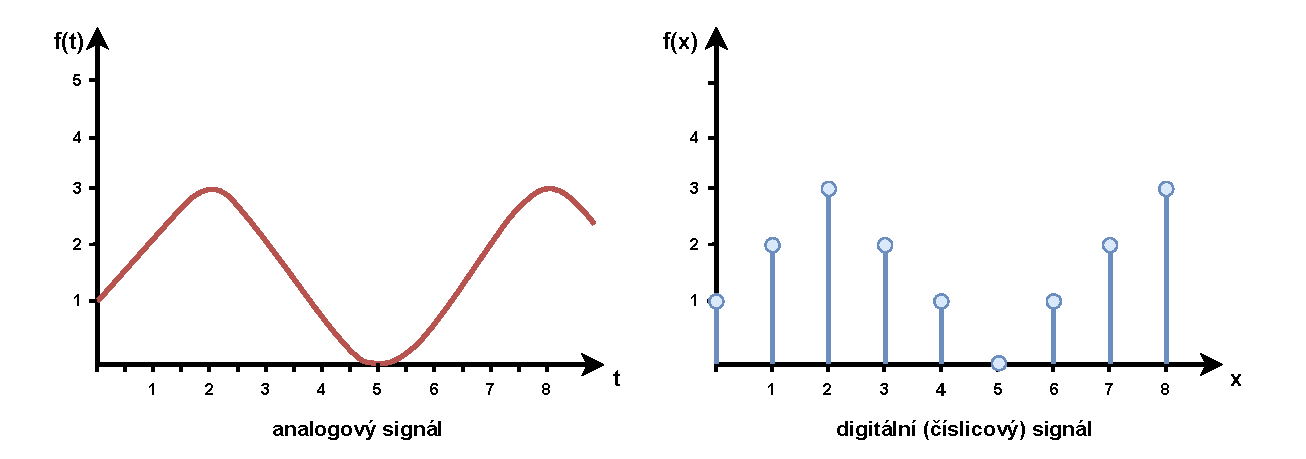
\includegraphics[width=1.00\textwidth]{obrazky-figures/digital_vs_analog.pdf}
    \caption{Průběh analogového a digitálního signálu}
    \label{fig:digital-vs-analog}
\end{figure}

U digitálních signálů je proces záznamu výrazně jednodušší, protože již nevyžaduje žádnou digitalizaci. Digitální data vstupující do záznamníku v podobě datového toku (data stream) skrz přijímací periferie. Tyto periferie jsou specializované nikoliv na konkrétní fyzikální veličinu (jak tomu bylo u analogových záznamových zařízení viz. kapitola \ref{zaznam}), ale na specifický komunikační protokol. Tedy jedna periferie může přenášet jak údaje o teplotě, vlhkosti, tak i cokoliv jiného (pokud je dodrženo správné komunikační rozhraní), přičemž povaha přenášených dat závisí na senzorech a zařízeních připojených k této periferii. Přijímaná data jsou tedy v přijímací periferii zpracovávána přímo ve své binární podobě, čímž odpadá celý proces potřeby provedení procesu digitalizace složeného z vzorkování, kvantizace a kódování. 

\newpage

Digitální záznam poskytuje mnoho výhod oproti svému analogovému protějšku. Primárně je to jeho flexibilita a efektivita při zpracování, ukládání a přenosu dat. Digitální data lze snadněji kopírovat, bezeztrátově přenášet a ukládat bez degradace kvality, což je pro záznamové systémy zásadní. Díky digitálnímu záznamu můžeme dnes i jednoduše analyzovat data, v porovnání s analogovým záznamem. Proto jsou dnes systémy s digitálním záznamem preferovanou volbou.

    
% TODO: Digitální záznamník může sloužit i pouze pro čistě PC programy? Pokud je zde nejak prijimaci periferie? To by slo primo do CPU
\subsection{Digitální záznamník}
\label{digitalni_zaznamik}
Digitální záznamník je dedikované zařízení nebo softwarový program určený ke sběru, zpracování a ukládání dat ve formě digitálního záznamu. Při pohledu na blokové diagramy digitálních záznamníků lze jejich strukturu rozdělit obecně do tří základních komponent, kterými jsou přijímající periferie, procesorové jádro a úložiště (viz. obrázek \ref{fig:common-digital-datalogger}). \cite{researchgate_general_dataloggger_multiple_sdcards, ieee_digital_sound_recorder_arm_sd_card, ieee_multi_connectivity_datalogger_sd_card}

Prvním klíčovým prvkem digitálního záznamníku je přijímající periferie, která slouží ke sběru vstupních dat. V závislosti na konkrétní aplikaci může tato komponenta zahrnovat různé typy vstupních rozhraní, jako jsou sériová rozhraní (UART, SPI, I\textsuperscript{2}C a další) síťová rozhraní (Ethernet, Wi-Fi, LoRa, CAN a další) nebo analogově-digitální převodníky.\footnote{Vyjímkou jsou specifické monitorovací programy mezi, které patří například Windows Task Manager, jež ke svému sběru dat využívají rozhraní pro programování aplikací tzv. kernel API. \cite{fourcore_win_process_birth}} \cite{ieee_digital_sound_recorder_arm_sd_card}


Druhým hlavním prvkem digitálního záznamníku je jádro výpočetní jednotky, zajišťující zpracování vstupních dat. Jádro může být jak součástí mikrokontroléru, respektive mikroprocesoru, tak i centrální výpočetní jednotky (CPU), které může mít v tomto případě na starosti jednoduché operace, jako je například přepočet hodnoty z analogově-digitálního převodníku na teplotu podle kalibrační křivky senzoru, přes filtrování šumu a doplňování časových značek k naměřeným vzorkům, až po pokročilé analýzy dat - například zpracování signálů pro EKG měření. \cite{springer_development_ECG_recorder}

\begin{figure}[h]
    \centering
    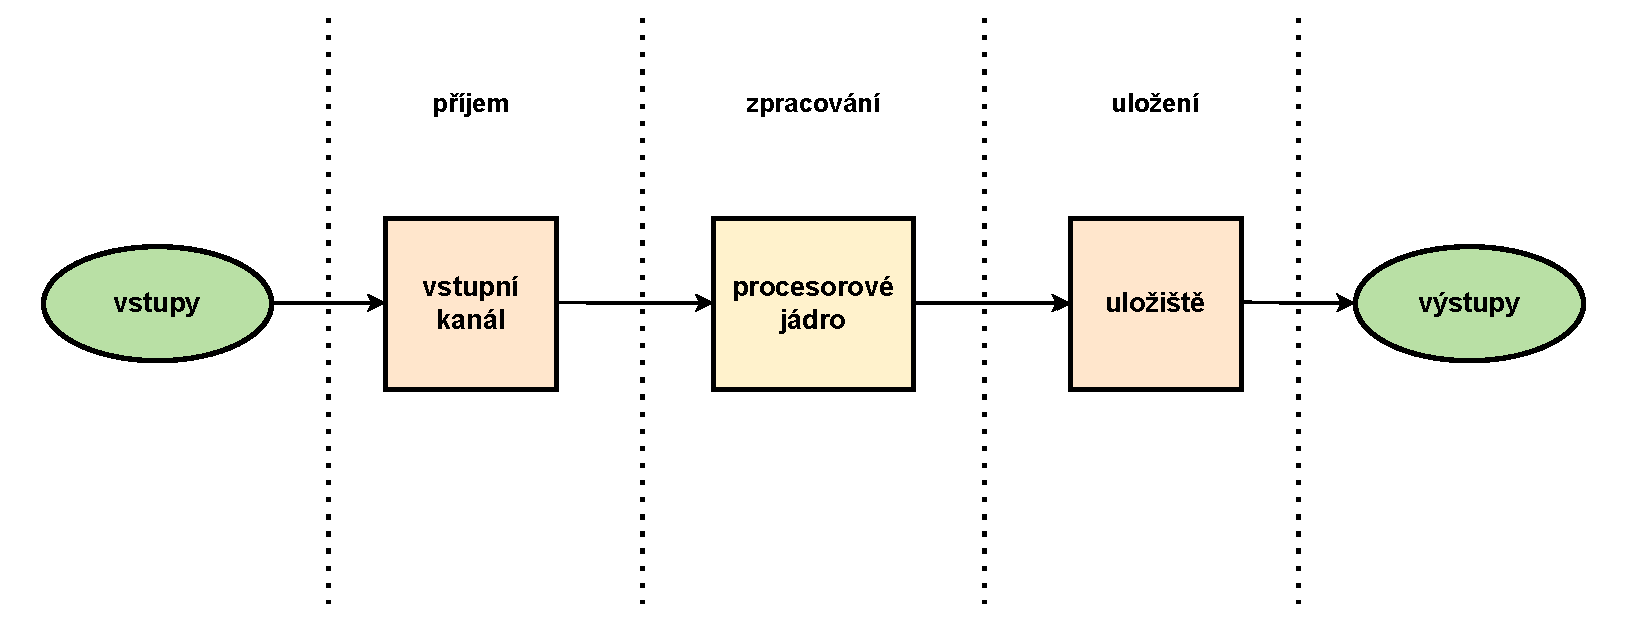
\includegraphics[width=1.00\textwidth]{obrazky-figures/common_digital_datalogger_scheme.pdf}
    \caption{Obecné schéma digitálního záznamníku}
    \label{fig:common-digital-datalogger}
\end{figure}

Poslední a také jednou z nejdůležitějších všeobecnou částí digitálního záznamníku je úložiště, kde jsou data ukládána pro pozdější přenos a zpracování (post-processing). Volba tohoto úložného prostoru závisí na požadavcích aplikace a rozsahu jejího využití, od osobních "hobby" projektů až po zařízení využívaná ve velkopodnikových prostředích, nasazována ve vysokých počtech. V závislosti na tom lze využít různé strategie, které jsou v koherenci s různými technologiemi od paměťových karet SD a eMMC přes interní RAM či flash paměti až po síťová úložiště a cloudové služby. V mnoha případech je také využíván hybridní přístup. Nashromžděná data mohou být nejprve ukládána do interní volatilní paměti záznamníku, jakou je třeba RAM úložiště (random access memory) a následně dávkově přenášena na trvalé médium (viz. kapitola \ref{fig:batch-processing}) v podobě lokálního či vzdáleného úložiště. Lze také přidat různé mezivrstvy pamětí, například feroelektrickou paměť s náhodným přístupem (FRAM), která je podrobněji rozebrána v kapitole \ref{fig:feram-1t-1c}, nebo jiné varianty nevolatilních pamětí s náhodným přístupem, případně další typy pamětí. \cite{rta_local_vs_cloud} 
% lokalni uloziste lze vyuzit i v kombinaci se vzdalznym ulozistem, kdy vznika hybridni architektura... 
% Zmiňované lokální uložiště lze navíc využít v kombinaci ze vzdáleným uložištem, kdy vzníká hybridní architektura, lze například data nejprve ukládat do interní paměti záznamníku (například RAM úložiště) a následně dávkově přenášena na trvalé médium (viz. kapitola \ref{fig:batch-processing}) nebo odesílána přes síť. \cite{rta_local_vs_cloud}

Digitální záznamník poskytuje výstupy, obvykle jimi jsou organizovaná data, která mohou být dále analyzována, vizualizována nebo zpracovávána jinými systémy. Jakou podobu mají výstupní data, tedy jaký je jejich formát, opět závisí na konkrétních požadavcích aplikace. Jedním z požadavků je volba dle typu úložiště, jedná-li se o lokální úložný prostor, například paměťovou kartu, využívají se velmi často typy formátů, jako třeba formát prostého textu (plain text) nebo binární formy. Databázová řešení typicky využívají formáty vycházející z relační nebo objektové reprezentace dat. Cloudová řešení naopak nabízejí daleko širší výběr, lze využít jak zmíněný prostý text, i binární formy, také lze ale využít objektové, textové formáty nebo formáty známé z databázových systémů. Dále záleží, jakým způsobem bude proveden přenos dat, pokud bude využita síťová komunikace, třeba pomocí MQTT či HTTP, je vhodné data uspořádat do serializované podoby, zatímco při zvolení přenosu po sériové lince je naopak vhodnější a efektivnější využít opět některý z binárních formátů. Důležitou roli hrají i požadavky na následný post-processing a interpretaci dat v jiných systémech či aplikacích k tomu určeným. Například pro náhled na digitální data z pohledu časových řad může být vhodné využít formáty, které jsou kompatibilní s například databázovými systémy k tomu určenými, jako je TimescaleDB, InfluxDB. V dalších případech může být efektivní využít knihovny pro zpracování a analýzu dat, například Pandas v prostředí Pythonu, které umožňují rychlou manipulaci s velkým objemem strukturovaných dat, v takových případech je tedy zase lepší strukturovat data podle formátu CSV. \cite{medium_optimalization_iot_data_storage_timescaledb}

Způsobů, jak lze digitální záznamník sestavit, existuje mnoho, přičemž volba konkrétní architektury závisí na požadavcích dané aplikace. Velice často se však skládá z výše představených komponent. 

\subsection{Digitální záznam v počítačovém systému}
Digitální záznamníky lze implementovat na počítačových systémech, jako jsou osobní počítače či servery, v podobě softwarových řešení, sloužící ke sběru, zpracování a potenciální archivaci dat. Tyto systémy obvykle také vycházejí ze struktury obecného číslicového záznamníku, popsaného v kapitole \ref{digitalni_zaznamik}. 

Vstupní data přicházejí často z periferií, jako je například síťová karta či sériové porty, ale mohou také pocházet ze "pseudo" zařízení obsahujících stavy aplikací běžících na daném počítači či speciálních API (např. již zmiňovaných kernel API). Procesor, který tato data příjímá, tak je obvykle nejen zpracovává, ale často i určitým způsobem vyhodnocuje, jelikož disponuje dostatečným výpočetním výkonem pro pokročilé operace. Výsledkem těchto úkonů procesoru nad daty bývají informace o aktuálním stavu sledovaného systému, které lze využít k monitorování a dalším rozhodovacím procesům. \cite{linux_in_action_log_and_monitoring}

% Wireshark: RAM -> Export
% Terminal or Serial Dataloggers (COM, RS232,...) -> Export to File, Excel or Database
% 
Podle požadavků aplikace a jejího zaměření se liší i způsob, jakým jsou data uchovávána. Mnohdy si tyto záznamníky odkládají data pouze dočasně do operační paměti RAM, to umožňuje sledovat pouze aktuální stav nebo krátkodobé trendy. Pro sledování dlouhodobých trendů je pak možné tyto záznamy exportovat na dlouhodobá uložiště, do různých typů souborů - CSV, XLS či speciálních formátů relevantních dané aplikaci. Také lze uplatnit koncept exportování do databázových systémů a cloudových služeb.

Takovýmto záznamníkem či rovnou monitorovacím systémem může být například program Wireshark, sloužící k záznamu síťové komunikace na síťových rozhraních počítačového systému. Wireshark pro záznam síťových rámců neboli paketů využívá vícevrstvou architekturu, data přicházejí přes síťovou kartu, čili to je hardwarová vrstva, pakety jsou následně zachytávány nebo dokonce i filtrovány pomocí WinPcap knihovny (Windows Packet Capture). Následně jdou přijatá data paketů zpracovávaná, identifikována (přiřazena konkrétnímu protokolu) a vizualizována na aplikační vrstvě. \cite{researchgate_wireshark_architecture, wireshark_architecture_diagram}

\begin{figure}[h]
    \centering
    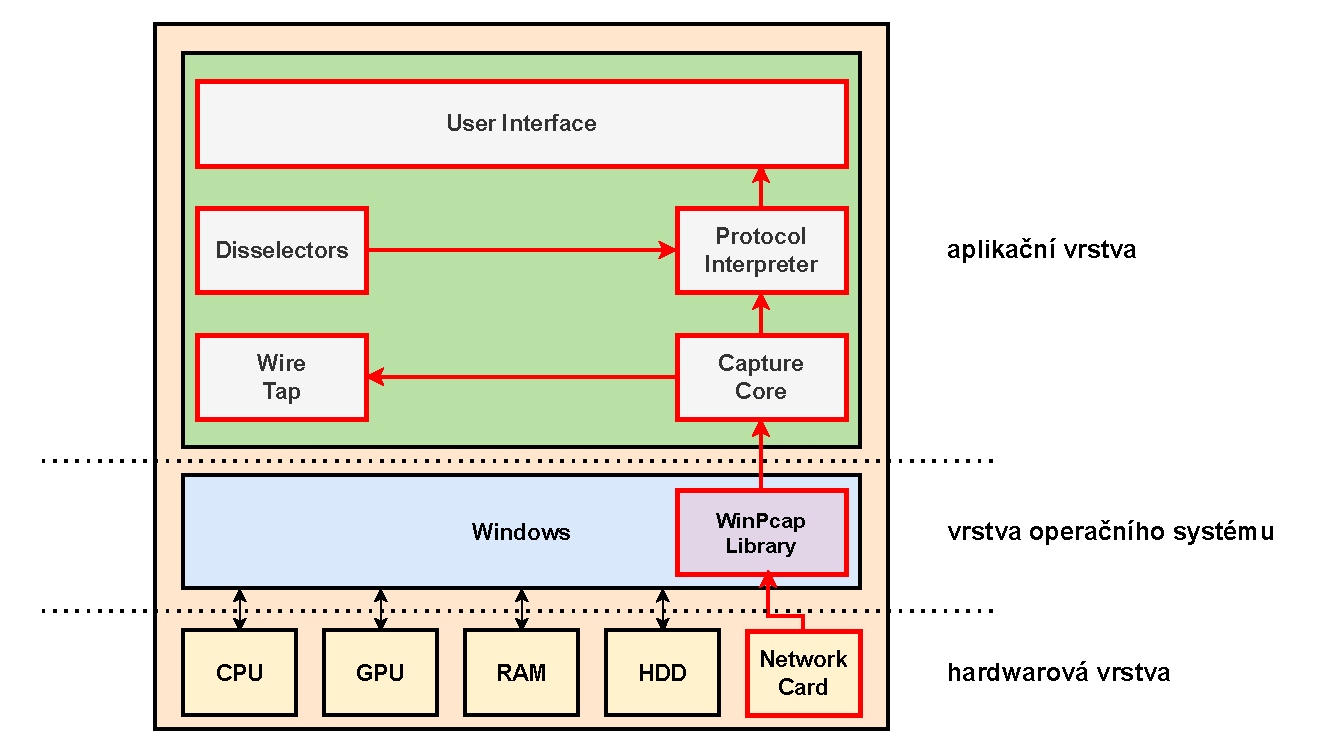
\includegraphics[width=1.00\textwidth]{obrazky-figures/wireshark.pdf}
    
    \caption{Schéma pokročilého digitálního záznamníku síťové komunikace - Wireshark \cite{researchgate_wireshark_architecture, winpcap_architecture}}
    \label{fig:computer-recorder}
\end{figure}

% Energie a udrzba?
Je nutné si uvědomit, že tyto záznamníky jsou především implementovány na strojích s relativně výkonnými hardwarovými prostředky, což je činí kolikrát až překvalifikované pro pouhé monitorování, proto se představují spíš roli doplňku (tj. hlavním účelem stroje není monitorování) například monitorování zmíněného síťového provozu, monitorování procesů běžících na daném stroji, pokročilé sériové záznamníky a terminály, či záznamníky speciálních rozhraní, jako je například HID (Human Interface Device).\footnote{Tyto záznamníky tedy neslouží pouze k monitorování samotného stroje na kterém jsou spuštěny, ale mohou také sledovat další připojená zařízení (a periferie), jakám je například sledování komunikace s mikrokontrolérem prostřednictvím sériového terminálu.}

Před implementací či použitím takového záznamníku je tedy vhodné si promyslet účel záznamníku. Klíčovou otázkou je, zda bude pro záznam nezbytné využít výpočetně výkonné zařízení (jakým je například stolní počítač), a zda zařízení bude sloužit výhradně k pořizování záznamů, nebo bude využito i k jiným úlohám. Jako alternativu k digitálnímu záznamníku implementovanému pro počítačový systém lze totiž využít záznamník v podobě dedikovaného zařízení (viz. kapitola \ref{digitalni_zaznamnik_mikroradic}). Možností, jak tedy implementovat digitální záznamník, je mnoho.
% Napsat zde proc neni mozne tento zpusob pouzit pro NXP monitorovani

% Používají se však trošku jiným způsob
%  Je nutné si uvědomit, že jádro mikrořadiče neposkytuje stejnou výpočetní sílu jako jádro procesoru.

\subsection{Digitální záznam na platformě mikrořadiče}
\label{digitalni_zaznamnik_mikroradic}
Digitální záznamníky nemusí být nutně implementovány na výkonných počítačových systémech, ale mohou být také realizovány jako vestavěné systémy postavené na mikrořadičích (MCU). Na rozdíl od záznamníků realizovaných na PC jsou však zaměřeny na oblasti, kde je potřeba určitým způsobem sbírat a ukládat data s důrazem na malou spotřebu energie, snadnou přenosnost a v některých případech nižší pořizovací cenu. Proto své uplatnění nacházejí v průmyslové automatizaci, IoT aplikacích, zdravotnických zařízeních a dalších oblastech. \cite{cas_industrial_dataloggers, madgetech_dataloggers_healthcare, springer_industry_monitoring, springer_healthcare_iot_monitoring}
% TODO: Mozna ten SPRINGER uz je MOC!

I tyto záznamníky také obvykle obsahují tři základní části obecného záznamníku představeného v kapitole \ref{digitalni_zaznamik}, které je možno libovolně rozšířit, jako je například zálohované napájení, signalizace stavu záznamníku a další funkční celky. Data vstupují do záznamníku prostřednictvím přijímacích periferií, která mohou pocházet z různých senzorů, ať už analogových či digitálních (tedy teplotních čidel, akcelerometrů nebo proudových snímačů a dalších) nebo z jiných pozorovaných zařízení. Vstupní periferie záznamníků mohou tvořit klasické komunikační rozhraní (UART, SPI, I\textsuperscript{2}C či I\textsuperscript{3}C,...) ale také bezdrátová rozhraní v podobě Wi-Fi, Bluetooth nebo analogově-digitální převodník.\footnote{Vstupních komunikačních je vícero, zde jsou zmíněna jen ty nejzákladnější} Tyto vstupní periferie mohou být přímo integrovány v mikrořadiči - například již uvedený analogově-digitální převodník, nebo mohou být připojeny externě ve formě samostatných modulů, které komunikují s MCU prostřednictvím již standardních rozhraní.

\begin{figure}[h]
    \centering
    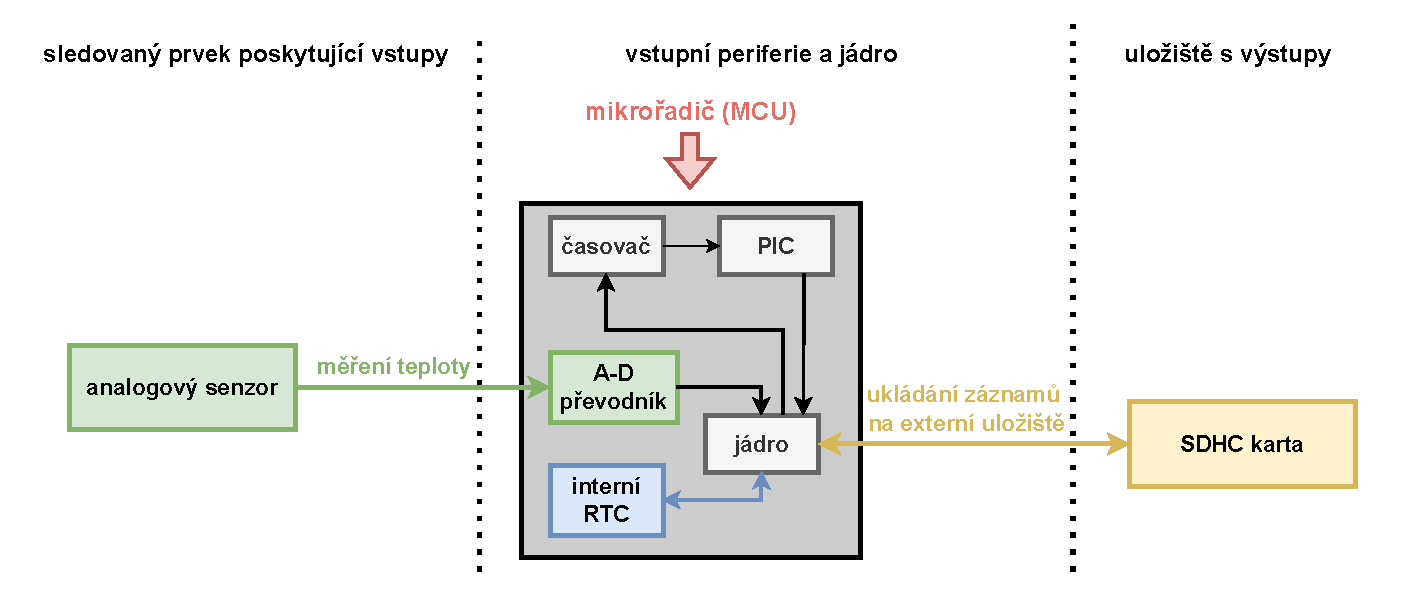
\includegraphics[width=1.00\textwidth]{obrazky-figures/recorder_mcu.pdf}
    
    \caption{Ukázka architektury digitálního záznamníku pro měření teploty}
    \label{fig:mcu-recorder}
\end{figure}

Vstupní data jsou následně zpracována jádrem mikrořadiče, které může provádět základní operace, jako je například převod číslicové hodnoty z ADC na teplotu, filtrování signálu, doplňování časových značek, nebo provádět i obtížnější operace, jako je výpočet tepu v případě měření srdečních aktivit a další.

Následně jsou digitální data ukládána do paměťového média. Zde jde zvolit obvykle dva přístupy s lokálním a nebo vzdáleným paměťovým uložištěm. Přístup s lokálním paměťovým uložištěm využívá sekundární uložiště, tedy nevolatilní úložiště, která zaručují perzistenci dat i po vypnutí záznamníku. Typickými zástupci těchto pamětí jsou například různé typy SD karet, USB Flash disky a další technologie využívající například technologie NAND a NOR flash paměti. Volatilní paměti, jako je například RAM, se v těchto aplikacích rovněž využívají, avšak výhradně pro krátkodobé uchování dat. V některých případech, například pokud jsou nevolatilní paměti organizovány do bloků (viz. \ref{davkove_zpracovani}), je výhodné nejprve dočasně ukládat data do RAM a teprve po naplnění bloku provést hromadný zápis do nevolatilní paměti, jelikož ukládání do nevolatilních uložišť přináší nové limitace, jakou je například rychlost zápisu,  omezený počet přepisovacích cyklů. Některá úložiště navíc vyžadují mazání celých bloků před opětovným zápisem. Krom lokálního paměťového média je však možné zvolit přístup se vzdáleným uložištěm v podobě databáze či cloudového systému, která však také mají své omezení.


\section{Klíčové koncepty digitálních záznamníku} 
\label{klicove_koncepty_digitalnich_zaznamniku}
Digitální záznamníky mohou být implementovány v podobě dedikovaného zařízení na platformě MCU, jak již bylo zmíněno, které dokáže poskytnout dobrý kompromis mezi cenou a výkonem. Na rozdíl od záznamníků realizovaných na výkonnějších platformách, jako jsou osobní počítače nebo jednodeskové počítače, však záznamníky postavené na MCU čelí určitým omezením daným dostupnými hardwarovými prostředky. Proto lze využít některé z optimalizačních technik, zaměřených na vhodnější využití dostupných zdrojů zařízení, které mohou vést k vyššímu výkonu, lepšímu využití dostupného paměťového prostoru nebo například i k lepší spotřebě.

\subsection{Vícenásobná vyrovnávací paměť (multiple-buffering)}
Jedním z častých konceptů využívaných v implementaci digitálních záznamníků je použití vícenásobné vyrovnávací paměti. Tento koncept je převážně známý díky algoritmům využívaným v oboru počítačové grafiky. Grafický čip musí zpracovat velké množství dat za krátký časový úsek, proto algoritmus zpracování dat využívá dvě vyrovnávací paměti - přední vyrovnávací paměť, takzvaný front-buffer, jež je využívána pro zobrazení aktuálního snímku, a zadní vyrovnávací paměť, ve které čip připravuje nový obsah. Výsledný obsah tak může být plynule vykreslen bez artefaktů a trhání. Jakmile je nový snímek kompletní, vyrovnávací paměti se vzájemně prohodí. \cite{double_buffering_model}

Obdobný mechanismus se využívá i v digitálních záznamnících, kde slouží k zajištění kontinuálního sběru dat bez výpadků. Zatímco jeden buffer přijímá nová digitální data ze vstupní periferie, druhý buffer je současně zpracováván nebo ukládán na úložné médium. Tím se minimalizuje riziko ztráty dat způsobené časovou prodlevou při jejich zpracování nebo zápisu.

\begin{figure}[h]
    \centering
    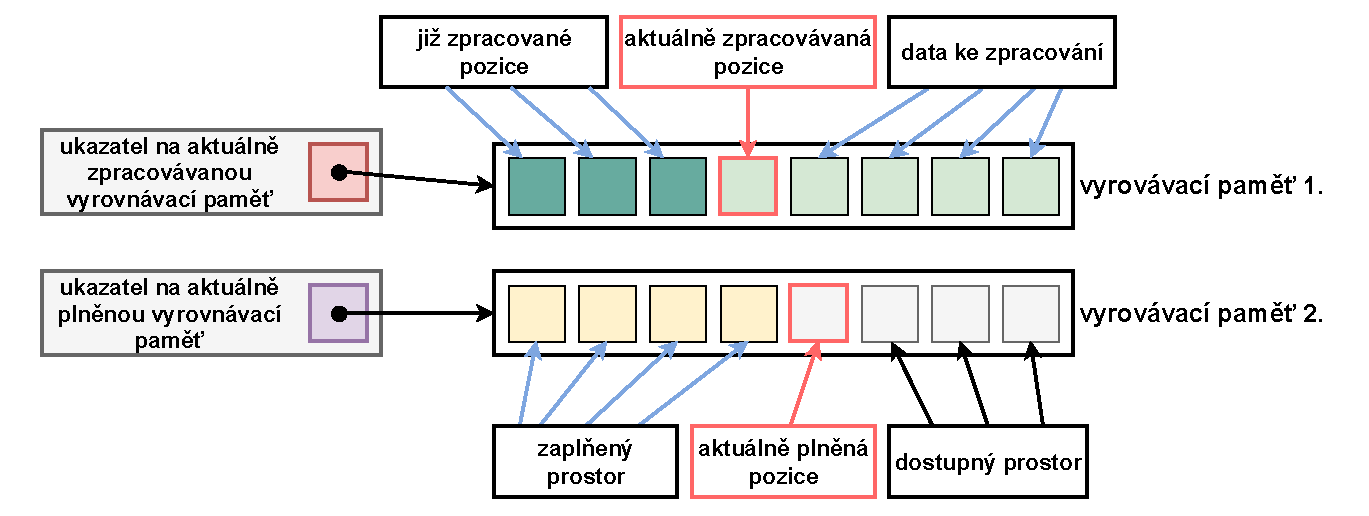
\includegraphics[width=1.00\textwidth]{obrazky-figures/multiple_buffering-1.pdf}
    
    \caption{Schéma principu práce s vícenásobnou vyrovnávací paměťí - náhodný stav}
    \label{fig:multiple-buffering-1}
\end{figure}

Důležitou vlastností tohoto přístupu je jeho nízká operační režijní náročnost. Plynulý chod zpracování dat je zajištěn bez nutnosti fyzického přenosu obsahu mezi vyrovnávacími pamětmi. Místo toho se využívají ukazatele (pointery), které směřují na počáteční adresy jednotlivých bufferů. Jakmile je sběrný buffer (Back Buffer) naplněn, ukazatele se prohodí~–~back buffer se stane zpracovávaným bufferem (Front Buffer) a původní front buffer se uvolní pro další sběr dat.

\begin{figure}[h]
    \centering
    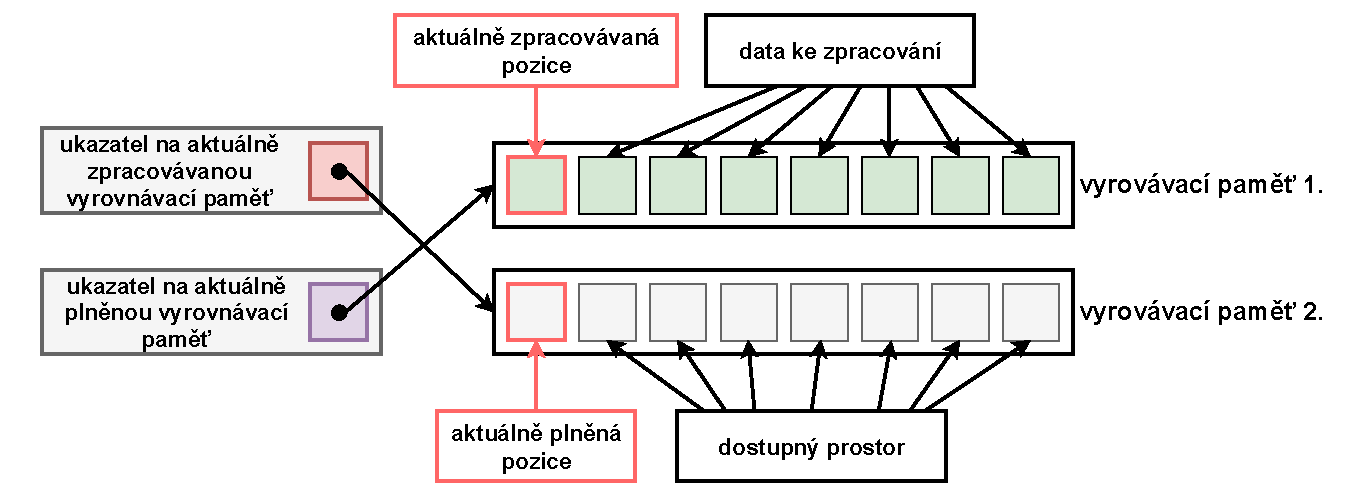
\includegraphics[width=1.00\textwidth]{obrazky-figures/multiple_buffering-2.pdf}
    
    \caption{Schéma principu práce s vícenásobnou vyrovnávací paměťí - přeřazení ukazatelů}
    \label{fig:multiple-buffering-2}
\end{figure}

Tato metoda nachází významné uplatnění zejména v systémech pracujících v reálném čase, kde dochází k příjmu velkého objemu dat v krátkých časových intervalech a kde doba zpracování nesmí překročit dobu sběru dat. Využitím vícenásobné vyrovnávací paměti se minimalizuje latence zpracování a současně se snižuje riziko přetečení paměťového prostoru. \cite{buffering_chang}

\newpage

Všechny přístupy využívané pro záznam dat mají své výhody i nevýhody a také tato metoda má své nevýhody/limitace, které je třeba zmínit. Primární nevýhodou je skutečnost, že vyrovnávací paměti jsou zpravidla implementovány softwarově, nikoliv hardwarově, což vede k zvýšeným nárokům na paměťové prostředky, obzvlášť v segmentu volatilní paměti (SRAM/DRAM) kde jsou buffery uložené. \cite{basics_of_digital_forensics}
% TODO: Je tedy vhodne si promyslet zda zdroje MCU budou dostacovat.

\subsection{Dávkové zpracování (batch processing)}
\label{davkove_zpracovani}
Další princip, využívaný v implementacích digitálních záznamníků, souvisí s typem uložišť, na které jsou získaná data zaznamenávána. Data jsou standardně dlouhodobě ukládána na některý z typů nevolatilních pamětí, které umožňují uchování dat i po odpojení napájení. Takovými uložišti jsou například NAND či NOR Flash paměti. Tyto typy paměti jsou organizovány do bloků (popřípadě stránek), přičemž bloky jsou následně rozděleny na menší jednotky zvané sektory. Velikost sektoru obvykle bývá 512 bajtů či 4096 bajtů, v závislosti na typu média a jeho architektuře. Tato bloková struktura umožňuje účinnou správu prostoru, které uložiště nabízí, ale současně vyžaduje specifický způsob zápisu/čtení dat, který je umožněn pouze na úrovni celých bloků. \cite{tech_target_nand_flash, non_volatile_memories}

Dávkové zpracování tohoto chování paměti využívá, data se tedy nejprve shromažďují ve volatilní paměti - například RAM, a teprve po naplnění určitého objemu (celého bloku či jeho násobku) dojde k jejich zápisu na dlouhodobé paměťové médium.

\begin{figure}[h]
    \centering
    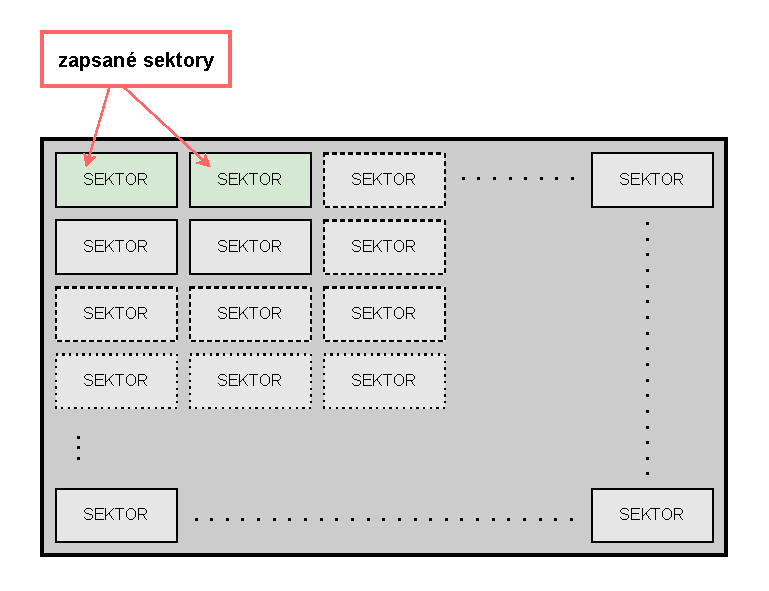
\includegraphics[width=0.75\textwidth]{obrazky-figures/batch_processing.pdf}
    
    \caption{Organizace bloku nevolatilní paměti \cite{ieee_relationships_among_region_segment_frame_and_cluster}}
    \label{fig:batch-processing}
\end{figure}

\newpage

\subsection{Cirkulární buffer}
\label{cirkularni_buffer}
Cirkulární buffer (circular buffer), někdy také označovaný jako kruhový nebo cylindrický buffer, je datová struktura, která funguje na principu FIFO fronty (First-In, First-Out) a považuje tuto paměť za kruhovou. Tento přístup je často využíván k řešení problému jednoho producenta a konzumenta (producent-consumer problem), kde jedno vlákno je konzument a druhé producent. Například ve vestavěných zařízeních, jedním z vláken je rutina obsluhy přerušení, která čte data ze senzoru a druhým vláknem je hlavní smyčka události. \cite{embedjournal_ring_buffer}


\begin{figure}[h]
    \centering
    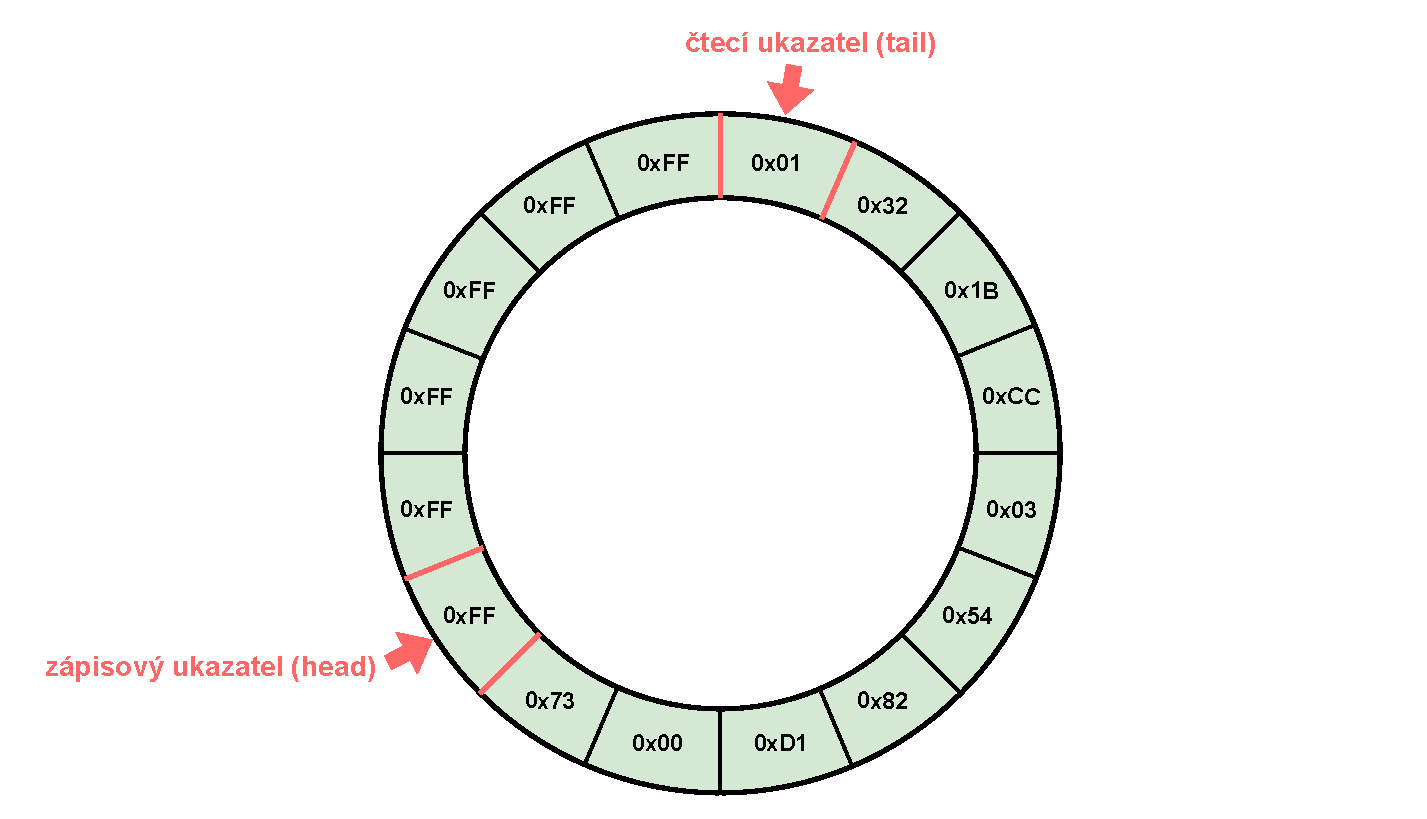
\includegraphics[width=1.00\textwidth]{obrazky-figures/circular_buffer.pdf}
    
    \caption{Cirkulární vyrovnávací paměť}
    \label{fig:circular-buffer}
\end{figure}

Princip činnosti cirkulárního bufferu spočívá v použití dvou ukazatelů - zápisový ukazatel (head) a čtecí ukazatel (tail). Ukazatel head vždy směřuje na pozici, kam bude zapisován následující prvek, zatímco ukazatel tail ukazuje na pozici, ze které bude čtena následující hodnota. Pokud ukazatel head dosáhne konce pole, vrací se na jeho začátek, čímž je zajištěna kruhová povaha struktury. Při plném bufferu lze zvolit dvě strategie – přepsání nejstarších dat nebo odmítnutí nových vstupů, přičemž výběr závisí na konkrétní aplikaci. \cite{embedjournal_ring_buffer, medium_ring_buffer}

Z hlediska časové složitosti nabízí cirkulární buffer konstantní časovou složitost - O(1) pro základní operace, jako je zápis (enqueue) a  čtení (dequeue). Tato efektivita je dána tím, že se při zápisu a čtení dat není potřeba přesouvat prvky v paměti, ale lze pouze inkrementovat ukazatele s využitím operace modulo. Pokud jde o prostorovou složitost, velikost cirkulárního bufferu je určena předem – zpravidla jde totiž o staticky alokované, to v tomto případě odpovídá složitosti O(n), kde n je maximální počet prvků, které může buffer pojmout. \cite{petrungaro_ring_buffer_complexity}

\subsection{Nízko-energetické režimy (low-power modes)}
\label{nizko_energeticke_rezimy}
Energetická efektivita je jedním z klíčových parametrů obecně vestavěných zařízení, tedy i digitálních záznamníků implementovaných na platformě MCU, zejména pokud jsou napájeny z baterií či jiných omezených zdrojů energie (například energy harvesting). Minimalizace spotřeby bývá v těchto případech realizována využitím nízkoenergetických režimů (low-power modes), které umožňují zařízení přejít do stavu s minimální energetickou náročností během nečinných period. V praxi mnoho digitálních záznamníků nemusí provádět měření a záznam dat nepřetržitě. Například záznamník teploty může v pravidelných intervalech provést měření, uložit naměřenou hodnotu, přejít do režimu nízké spotřeby a po uplynutí definovaného časového intervalu nebo při vyskytnutí speciální události přejít do aktivního režimu. \cite{analog_devices_low_power_modes}

Průběh takového cyklického chování spotřeby mikrokontroléru, kde se střídají fáze měření a spánku s pravidelnou periodou měření teploty, je znázorněn na obrázku \ref{fig:low-power-modes} níže.

\begin{figure}[h]
    \centering
    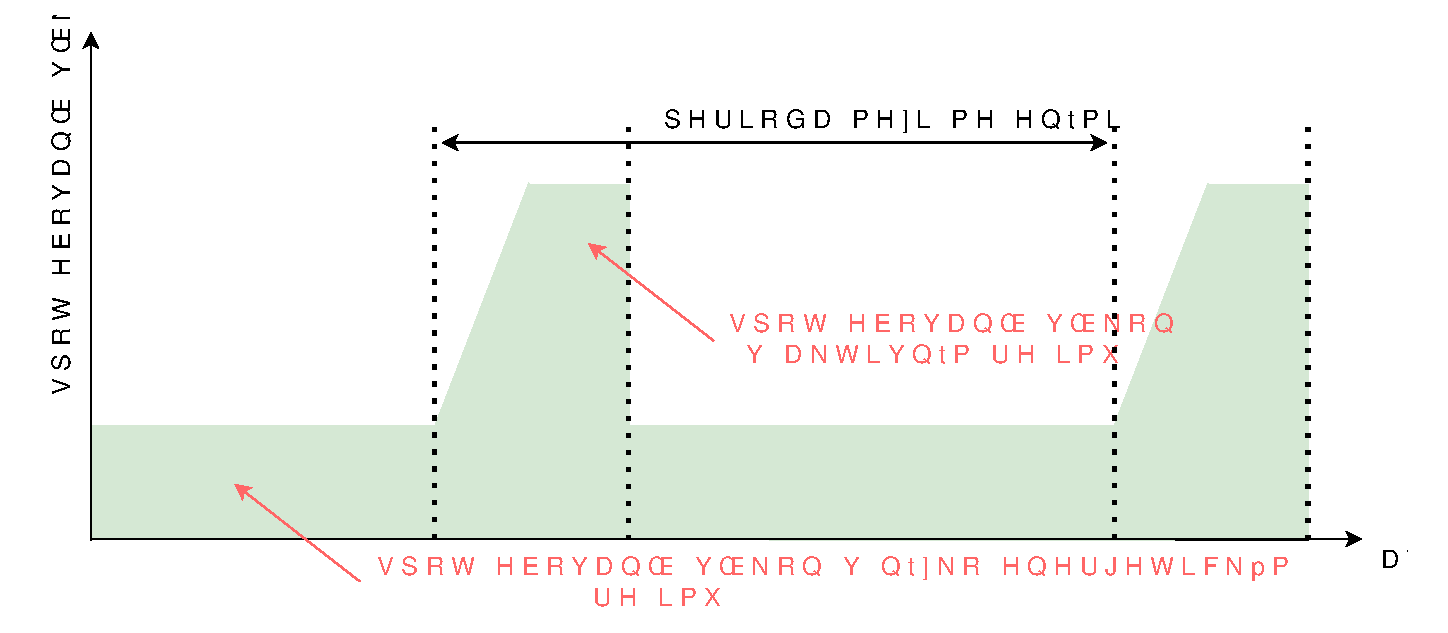
\includegraphics[width=1.00\textwidth]{obrazky-figures/low_power_modes-cz.pdf}
    
    \caption{Graf znázorňujíci dynamiku spotřeby mikrokontroléru v průběhu času při využití aktivního a nízkoenergetického režimu}
    \label{fig:low-power-modes}
\end{figure}

Ačkoliv nízkoenergetické režimy přinášejí značné úspory energie a jsou nezbytné pro zařízení napájená z baterií, u dataloggerů s velkým objemem zaznamenávaných dat mohou představovat významná omezení. Tyto režimy sice snižují energetickou náročnost systému, avšak zároveň omezují schopnost mikrokontroléru rychle reagovat na události. Spánkové stavy, které minimalizují spotřebu energie, často vedou k delšímu zpoždění při probuzení a nižší dostupnosti kritických periferií. V aplikacích, kde je vyžadována okamžitá odezva na externí podněty nebo nepřetržité zpracování velkého množství dat, může tento faktor negativně ovlivnit spolehlivost a efektivitu záznamníku. \cite{embedded_low_power_modes}

V těchto případech je proto nutné zvážit provozní podmínky a očekávanou dostupnost systému. Pokud záznamník pracuje s velkým datovým tokem a má možnost být připojen po dobu záznamu stále k externímu napájení, může být výhodnější upustit od implementace nízkoenergetických režimů a místo toho optimalizovat architekturu systému pro nepřetržitý provoz s důrazem na výkon a rychlou odezvu. \cite{analog_devices_low_power_modes}

% Normostrany = 11.34

\section{Způsoby zápisu dat}
Podobně jako jsou podstatné uložiště, na které jsou zaznamenaná data získaná, je také důležitá práce s tímto uložištěm. Záznamníky dat musí být navrženy tak, aby umožnily spolehlivé ukládání získaných dat, které by mělo být efektivní ve smyslu rychlosti a šetrné pro zvýšení životnosti uložiště. V této kapitole jsou popsány tři různé způsoby ukládání dat, přímý zápis na lokální úložiště, ukládání prostřednictvím mezivrstvy s FRAM pamětí a využití vzdálených úložišť. Každá z těchto metod má své specifické výhody a omezení, které určují její vhodnost pro konkrétní aplikace.

\subsection{Přímý zápis na permanentní uložiště}
Přímý zápis na permanentní úložiště představuje nejjednodušší a nejpřímější metodu ukládání dat. V tomto případě jsou zaznamenaná data ihned zapisována na nevolatilní paměťové médium, jako je SD karta, eMMC, USB Flash disk nebo NAND Flash čip. Tento způsob eliminuje potřebu mezivrstvy mezi záznamníkem a úložištěm, čímž se minimalizuje latence a zjednodušuje celková implementace.

\begin{figure}[h]
    \centering
    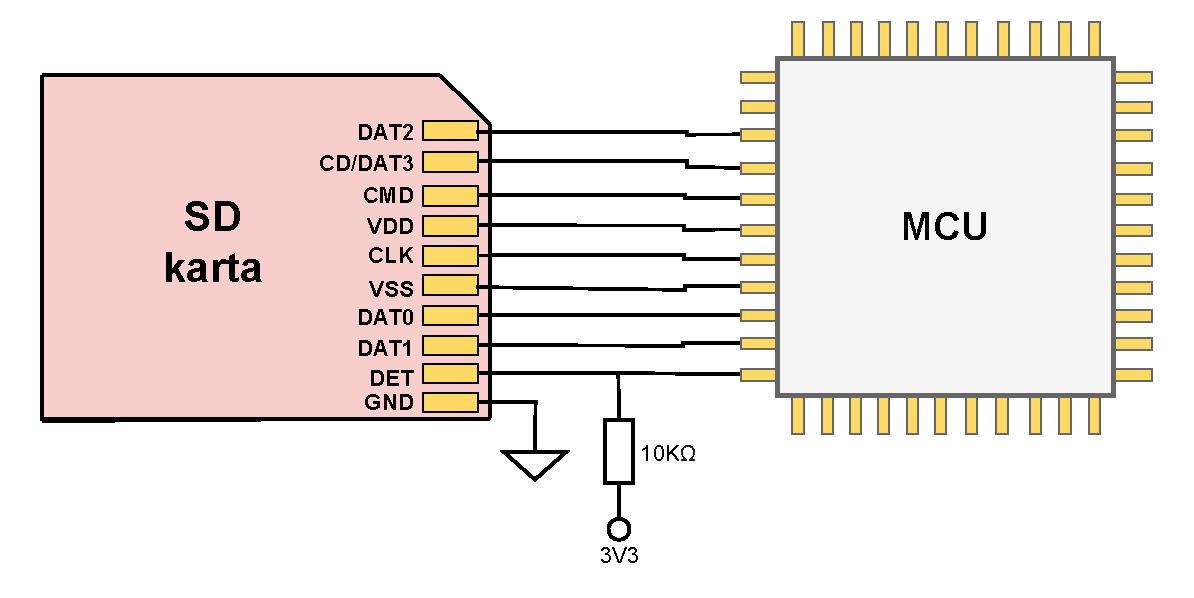
\includegraphics[width=1.00\textwidth]{obrazky-figures/forward_write.pdf}
    
    \caption{Přímý zápis na permanentní uložiště s SDHC kartou za pomocí čtyř pinové datové sběrnice}
    \label{fig:forward-write}
\end{figure}

Hlavní výhodou této metody je její jednoduchost a okamžitá perzistence dat. Data jsou ukládána přímo na trvalé úložiště a nehrozí tak jejich ztráta při výpadku napájení. To je zvláště výhodné v záznamnících, které zapisují drobné množství dat, kde se data neměří neustále, ale jednou za danou periodu uvedenou v kapitole \ref{nizko_energeticke_rezimy}, například v environmentálních záznamnících monitorujících teplotu nebo vlhkost.

Problémem tohoto principu je však častý zápis na paměťové médium. Proto, aby se předešlo nadměrnému opotřebení uložiště a zvýšila se efektivita zápisu, využívá se mnohdy současně metoda dávkového zpracování (batch processing) zmíněná v kapitole \ref{davkove_zpracovani}. Data jsou krátkodobě uložena ve volatilním uložišti, a jakmile jich je nashromážděno dostatek, tak jsou přepsána do dlouhodobé nevolatilní paměti. To ale přináší i nové problémy, kdy hodnoty uložené v neperzistentním uložišti jsou vystavena riziku ztráty v případě ztráty napájecího napětí.

\subsection{Zápis na permanentní uložiště přes mezivrstvu s FRAM paměti}
Alternativní volbou k přímému zápisu na permanentní úložiště je využití mezivrstvy ve formě FRAM (Ferroelectric Random Access Memory). FRAM je nevolatilní paměť, jež kombinuje výhody rychlé volatilní RAM paměti a perzistentního úložiště.

Ve feroelektrické RAM paměti (FRAM/FeRAM) jsou data ukládána pomocí změny polarizace feroelektrického materiálu v paměťové buňce. Jednotlivé buňky se skládají podobně jako je tomu u dynamické RAM (DRAM), z jednoho tranzistoru a jednoho feroelektrického kondenzátoru (1T-1C). Na rozdíl však od DRAM, kde je informace uchovávána jako elektrický náboj v lineárním dielektriku, FeRAM využívá feroelektrický materiál, jakým je třeba titaničitan olovnatý (PZT), který vykazuje hysterezní chování. Jakmile je aktivní elektrické pole, dipóly se v krystalové mřížce přeuspořádají do jednoho ze dvou stabilních stavů odpovídajících binárním hodnotám nula či jedna a tento stav zůstává zachován i po odeznění elektrického pole. \cite{ieee_feram_ultra_high_density_embedded_mem}

\begin{figure}[h]
    \centering
    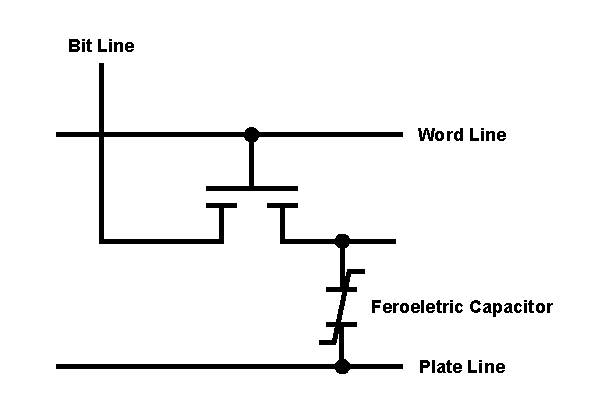
\includegraphics[width=0.70\textwidth]{obrazky-figures/fram_t1-c1.pdf}
    
    \caption{Struktura 1T-1C feroelektrické RAM paměti (FeRAM) \cite{researchgate_nonvolatile_memory_technologies}}
    \label{fig:feram-1t-1c}
\end{figure}
% Word Line - slovni linka, pomoci ni se aktivuje pristup k jednomu radku bunek, aktivuje se pri cteni ci zapisu konkretniho slova ci bajtu 
% Word Line 
% Bit Line - bitova linka, vertikalni spojeni pametovych bunek, kazdy sloupec ma svoji bitovou linku
% Plate Line - použita k vytvoření elektrického pole, které umožňuje přepólování feroelektrického materiálu

FRAM lze v dedikovaném digitálním záznamníku využít jako takzvanou mezivrstvu neboli vyrovnávací paměť, pomocí které lze optimalizovat zápisy na konečné dlouhodobé úložiště. Jak jsou tedy data záznamníkem postupně sbírána, tak mohou být postupně či po blocích zapisována do této mezivrstvy. Pokud je následně vyrovnávací paměť FRAM dostatečně zaplněna, její obsah je dávkově přenesen na dohodnuté trvalé úložiště, a tento cyklus se opakuje. 


% navíc nevolatilní, diky usporadanym dipolum, ktere bylo zajisteno aktivnim elektrickem poli 
Použití FRAM jako vyrovnávací paměti přináší několik výhod. Jedním z hlavních přínosů je snížení opotřebení hlavního úložiště, eliminován je totiž častý zápis po malých blocích dat, který zbytečně opotřebovává koncová nevolatilní úložiště typu flash, která mají omezený počet přepisovacích cyklů. Další výhodou je velice rychlý zápis oproti flash pamětem, obvykle trvá zápis na FRAM v řádu nanosekund, což je řádově rychlejší než srovnávané flash paměti, na kterých zápis trvá typicky v řádu mikrosekund až milisekund. FRAM je navíc nevolatilní, což znamená, že i v případě výpadku napájecího napětí zůstávají zaznamenaná data na feroelektrickém uložišti zachována, čímž se eliminuje potřeba dodatečných opatření k ochraně dat, jako jsou záložní baterie nebo superkondenzátory.

\subsection{Zápis na vzdálené uložiště}
\label{zapis_na_vzdalene_uloziste}
Pro dlouhodobé uložení dat lze také využít vzdálená uložiště, jakými jsou databáze či cloudy. Lze tak využít jednotného uložiště pro velké množství digitálních záznamníků a eliminovat tak potřebu lokálních, nevolatilních paměťových médií. Zmiňované jednotné uložiště může být jak centrální server, tak i distribuovaná síťová soustava, umožňující uložení daleko většího množství dat, než může nabídnout lokální uložiště.

% Neni to tak ze CoAP a MQTT jsou si rovny, MQTT se hodi spis na komunikaci, kde Tx a Rx jsou synchronizovany, kde komunikace probiha casto asynchronne, jedno zarizeni data vysila a ostatni je mohou odebirat a nasledne prijimat, takhle jde udelat efektivni komunikaci bez nutnosti synchronizace
% CoAP, je zase spis pro format dotaz-odpoved mimikuje HTTP
V praxi dedikovaný záznamník, který data buď přímo zpracovává, nebo je dočasně uchovává ve volatilní paměti, využívá síťové rozhraní k jejich přenosu do vzdáleného úložiště. Přenos probíhá obvykle prostřednictvím aplikačních síťových protokolů postavených nad transportním protokolem TCP (Transmission Control Protocol), jakým je MQTT, nebo nad protokolem UDP, nad kterým je postaven třeba protokol CoAP. Každý z uvedených zástupců poskytuje trošku odlišnou funkcionalitu. MQTT je vhodnější pro komunikaci, kde odesílatel a příjemce jsou synchronizováni a dialog probíhá asynchronně. Vysílatel tedy odesílá data a ostatní zařízení mohou začít. Zato CoAP zase prosazuje formát komunikace typu dotaz-odpověď, kterým mimikuje HTTP. \cite{emq_mqtt_vs_coap}


\begin{figure}[h]
    \centering
    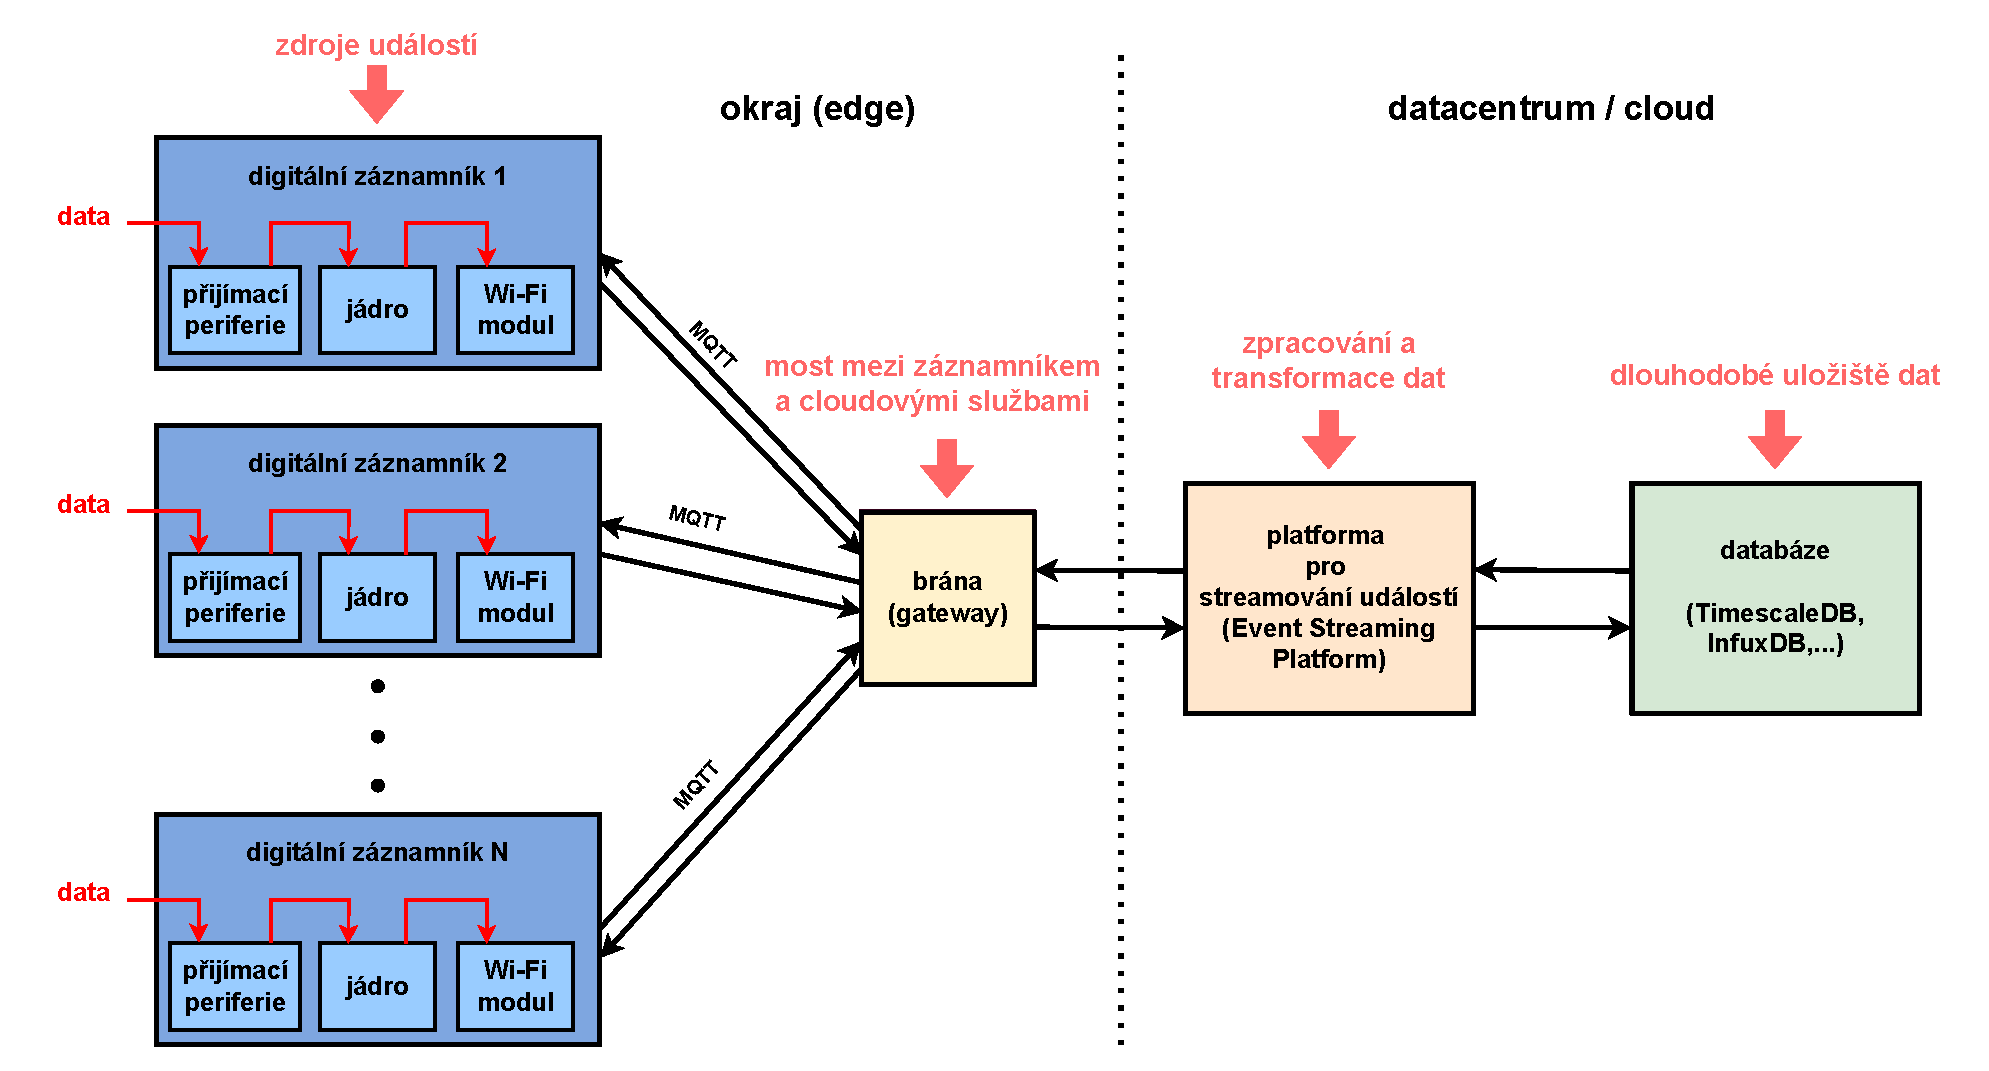
\includegraphics[width=1.00\textwidth]{obrazky-figures/advanced_architecture_of_datalogging.pdf}
    
    \caption{Schéma pokročilého digitálního záznamníkíku s cloudovým uložištěm postavený na streamingové platformě Kafka \cite{confluent_advanced_datalogging, influxdata_advanced_datalogging_mmqt}}
    \label{fig:advanced-architecture-of-datalogging}
\end{figure}

% Pouzivaji se treba v pokrocilych systemech kdy uz je mozne z dat neco i odvozovat, napriklad venku je pekne a v dobe je 25 stupnu tak trosku pootevru okna.

Následně jsou data ukládána na již zmiňované databázové servery či cloudové služby. Databázové servery mohou být postaveny na různých technologiích v závislosti na typu dat a požadavcích na jejich zpracování. Často jsou využívány systémy, které umožňují pracovat s daty ve formátu časových řad, což jsou sekvence datových bodů zaznamenávaných ať už v pravidelných či nepravidelných časových intervalech. Na taková data může být tedy vhodné využít například InfluxDB nebo TimescaleDB.\footnote{Možné je také zvolit relační databáze, ale ty jsou u digitální záznamníků méně časté.} Cloudová řešení jsou pak objektová uložiště, kde jsou data ukládána v podobě souborů či binárních objektů. Zároveň tyto služby umožňují krom samotného uložení přidat i analytickou vrstvu, která umožňuje zpracování dat v reálném čase a reagovat tak na aktuální stav. K tomuto účelu pak lze využít třeba streamovací platformy, jakými jsou Apache Kafka (viz. obrázek \ref{fig:advanced-architecture-of-datalogging} a AWS Kinesis. \cite{springer_analysis_time_series_db_edge_computing}

Výhodou tohoto přístupu je především možnost centralizovaného ukládání a zpracování dat, to se hodí při velkých množstvích digitálních záznamníků, jelikož v takovémto případě nechceme manuálně kontrolovat všechna zařízení a postupně z nich extrahovat získaná data. Další výhodou je možnost reagovat na aktuální stav či odvozovat některé skutečnosti. Je tedy třeba možné v chytrých domácnostech automaticky upravit výkon klimatizace nebo vytápění na základě dat ze senzorů teploty a vlhkosti. \cite{springer_analysis_time_series_db_edge_computing}

Tento přístup se hodí pro digitální záznamníky operující ve známých prostředích, kterým je třeba zmiňovaná chytrá domácnost či továrna, jelikož je potřeba zaručit stabilní připojení k síti. Pokud by měl záznamník cestovat různě po světě, bylo by nutné jej na každém novém místě připojit k Wi-Fi síti či Ethernetu, nebo by jej bylo nutné koncipovat jako digitální záznamník se SIM kartou, pomocí které by byl zajištěn přístup k mobilní síti. Dále je důležité mít i koncipovanou komplexní infrastrukturu, v níž je zajištěn bezpečný přenos dat. Pro tento síťový přenos je třeba přidat další úroveň zabezpečení, která zajistí autentizaci, šifrování, integritu dat a případně další bezpečnostní prvky. S bezpečností souvisí také nezbytnost aby zařízení disponovalo zdroje pro běh plnohodnotného TCP/IP modulu
(stack), díky kterého bude možné využít bezpečností prvky jako je například SSL/TLS a který je zároveň potřebný pro již zmíněný protokol MQTT, běžící nad transportním protokolem TCP.


\chapter{Návrh digitálního záznamníku}
\label{navrh_digitalniho_zaznamniku}

\section{Existující řešení digitálních záznamníku}
Jak již bylo zmíněno v předchozích kapitolách, problematika záznamu dat provází lidstvo od nepaměti. Stejně tak samotné záznamníky dat nejsou novým tématem a v praxi již existuje celá řada produkčních řešení zaměřených na záznam různých typů dat. Tato kapitola je věnována popisu některých dostupných řešení, konkrétně záznamníkům zaměřeným na záznam datových toků zmíněných v kapitole \ref{digitalni_zaznam_dat}, mezi které se bude řadit i výsledné zařízení, které jsem navrhl, implementoval a popsal v této bakalářské práci. 


\subsection{OpenLog Serial Data Logger}
\label{openlog_serial_datalogger_module}
Prvním z vybraných existujících záznamníků je modul OpenLog, který je kompaktní a snadno použitelné zařízení pro záznam sériové komunikace, který vyvinula společnost SparkFun. Tento záznamník běží na osmibitovém mikrokontroléru ATmega328P taktovaném na 16 MHz a je navržen tak, aby umožnil přímý záznam sériové komunikace na microSD kartu s podporou až do velikosti 32 GB a bez nutnosti složitější konfigurace. \cite{sparkfun_openlog_tutorial}

\begin{figure}[h]
    \centering
    \includegraphics[width=0.85\textwidth]{obrazky-figures/sparkfun-openlog.png}
    
    \caption{Digitální záznamník SparkFun Openlog \cite{cirkit_openlog}}
    \label{fig:sparkfun-openlog}
\end{figure}

Tento záznamník je vhodný na jednoduché projekty, hobby projekty, či prototypování, záznamník OpenLog lze totiž snadno použít v systémech postavených například na nepájivém poli. Záznamník je vhodný k monitorování systémů, které již provedly předzpracování dat ze svých datových zdrojů a potřebují data je
n uložit (viz. obrázek \ref{fig:sparkfun-openlog-use-case}). Obvykle je v tomto případě hlavní mikrokontrolér, který přijímá monitorovaná data (např. z GPS modulu) a následně je jakýmsi způsobem zpracovává a formátuje je do koncové podoby a následně je posílá po sériové lince na bázi UART komunikace do Openlog modulu. Záznamník si data následně ukládá do vyrovnávací paměti ve volatilní RAM paměti a jakmile se tento buffer naplní (viz. kapitola \ref{davkove_zpracovani}), tedy nasbírá 512 bajtů, tak je zapíše do micro SD karty. \cite{cirkit_openlog}

\begin{figure}[h]
    \centering
    \includegraphics[width=0.85\textwidth]{obrazky-figures/sparkfun-openlog-use-case.png}
    
    \caption{Sledovací zařízení GPS se záznamem dat \cite{cirkit_openlog}}
    \label{fig:sparkfun-openlog-use-case}
\end{figure}

Nevýhodou tohoto záznamníku je, že hlavní mikrokontrolér, který zpracovává data a posílá data následně do záznamníků, musí být aplikačně předchystán k tomuto účelu, což zvyšuje režii (overhead) navíc. Toto řídící MCU musí buď pomocí příkazů nastavit parametry záznamu, jako je baudrate, vytvoření souboru, přidání dat do souboru a další funkcionality, nebo je třeba využít konfigurační soubor uložený na SD kartě. Bohužel po nastavení v konfiguračním souboru je nutné provést restart záznamníku, než se provede aktualizace nastavení. Záznamník podporuje zápis na SD karty s kapacitou od 64 MB do 32 GB se souborovými systémy, nicméně je nutné tuto SD kartu zformátovat na zařízeních s operačním systémem Windows. Další nevýhodou tohoto záznamníku je, že nepodporuje přístup na SD kartu bez nutnosti vyjmutí fyzického uložiště.

\subsection{Keeylog AirDrive Serial Logger}
\label{keelog_airdrive_serial_datalogger}
Dalším takovým řešením je AirDrive Serial Logger, vyvinutý společností Keelog. Toto zařízení je moderní digitální záznamník poskytující bezdrátový přístup k datům, který umožňuje záznam sériových dat pomocí komunikačního standardu RS-232 či RS-485. Na rozdíl od tradičních řešení, která ukládají data pouze na lokální úložiště, nabízí tento záznamník konektivitu k Wi-Fi síti, čímž umožňuje vzdálený přístup k uloženým datům bez nutnosti vyjmutí fyzického média a manipulace s tímto zařízením. Společnost Keelog poskytuje vícero variant AirDrive záznamníků, které se liší poskytnutými funkcionalitami. Hlavním rozdílem mezi jednotlivými verzemi je odlišný přístup k získaným datům, základní verze pracuje jako Wi-Fi hotspot, zatímco verze Pro a Max umožňují připojení do existující Wi-Fi sítě a také odesílání e-mailových reportů, časové razítkování záznamů nebo dokonce živé streamování dat. V čem se naopak zmíněné verze neliší, je velikostí interní paměti, která činí 16 GB, jež je uživatelsky přístupná i jako USB flash disk s rychlostí až 480 Mbps. Zařízení jako AirDrive nachází uplatnění zejména v průmyslovém monitorování, zpětném inženýrství sériových protokolů, zálohování dat z platebních terminálů nebo sběru dat ze senzorových systémů. \cite{keelog_airdrive_serial_datalogger, keelog_airdrive_serial_datalogger_max, keelog_airdrive_serial_datalogger_pro}

\begin{figure}[h]
    \centering
    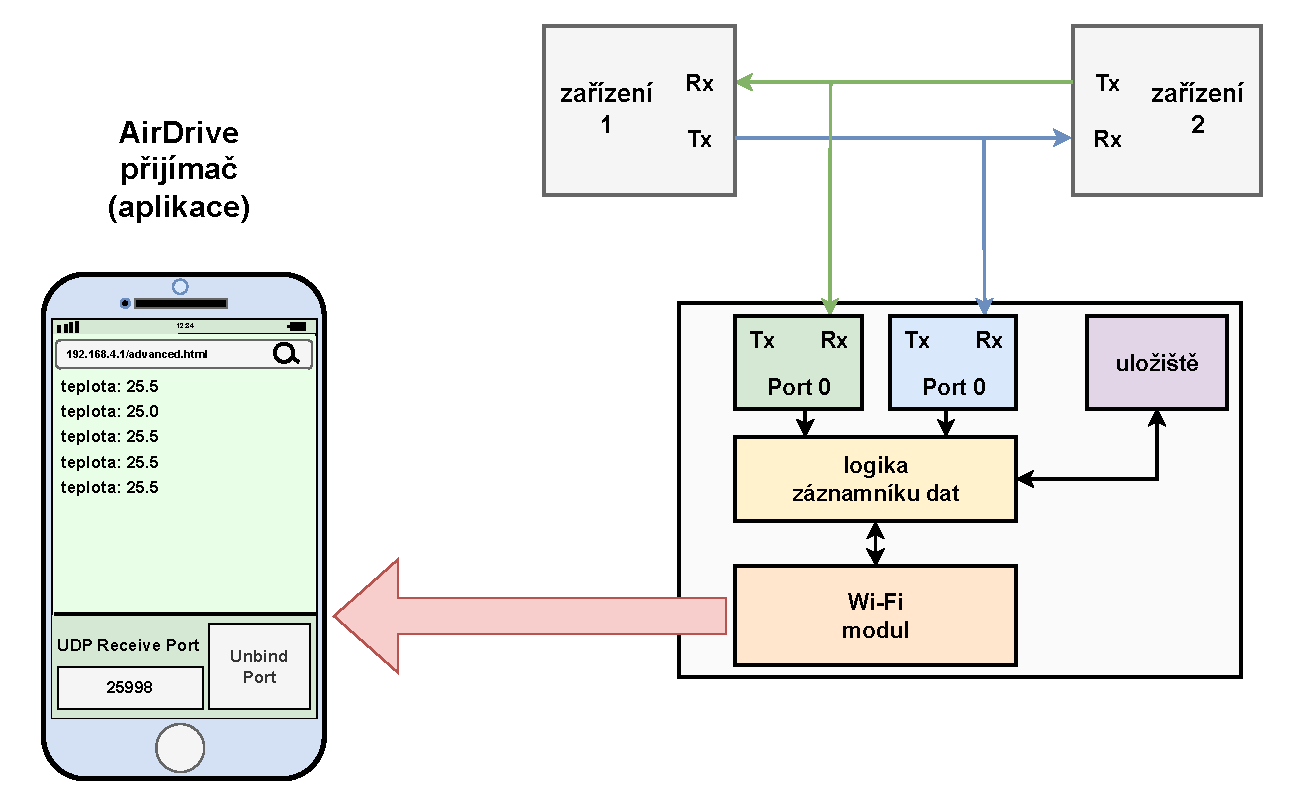
\includegraphics[width=0.90\textwidth]{obrazky-figures/keeylog_airdrive_serial_logger-cz.pdf}
    
    \caption{Keeylog AirDrive Serial Logger s přístupem k datům přes webové rozhraní \cite{keelog_airdrive_serial_datalogger, keelog_airdrive_serial_datalogger_scheme}}
    \label{fig:keelog-airdrive-serial-datalogger}
\end{figure}

Hlavní výhodou AirDrive Serial Loggeru je již zmiňovaná poskytovaná bezdrátová konektivita, která umožňuje přístup k datům z jakéhokoliv zařízení s Wi-Fi připojením, což se může hodit zejména v průmyslových  prostředích, kde může být velký počet takovýchto zařízení a získaná data tak mohou být hromaděna na jednom místě. Tímto centrálním bodem může být například cloudové úložiště nebo serverová databáze (viz. kapitola \ref{zapis_na_vzdalene_uloziste}), kam mohou být data pravidelně odesílána a následně mohou být analyzována. Tento záznamník také podporuje možnost konfigurace pomocí souboru CONFIG.TXT, ve kterém je možné nastavit, s jakou frekvencí budou získaná data odesílána do koncového úložiště. Pro a Max verze umožňují také nastavit tzv. živé vysílání (live streaming), při němž data mohou být monitorována a analyzována v reálném čase. Možné je také k datům přiřazovat časová razítka (timestamps), to se může hodit pro monitorování systémů, jejichž chování se chystáme porovnávat vůči jiným systémům a je tedy nutné si synchronizovat dva záznamy z různých zařízení. \cite{keelog_airdrive_serial_datalogger}

Navzdory svým pokročilým funkcím má AirDrive Serial Logger i několik nevýhod. Jednou z nich je omezení na standardy RS-232 a RS-485, které sice stále nacházejí uplatnění v průmyslových a v řadě dalších systémů, avšak v některých ostatních zařízeních je pro připojení k jiným rozhraním nutné využít sériové převodníky. Jelikož tyto standardy využívají asynchronní sériovou komunikaci (UART), není možné s tímto záznamníkem přímo zaznamenávat data z jiných běžných komunikačních sběrnic, jako jsou I\textsuperscript{2}C, SPI, USB, CAN a také nepodporuje možnost digitalizace pomocí A-D převodníku. Tím se omezuje jeho univerzálnost a možnost použití v širším spektru aplikací. Další limitací je maximální přijímací přenosová rychlost UART (baud rate), která dosahuje pouze 115200 bps. To je například nevyhovující pro monitorování systémů bezdrátového nabíjení společnosti NXP Semiconductors, kde se komunikace probíhá s vyšší komunikační rychlostí. \cite{keelog_airdrive_serial_datalogger}

\subsection{Anticyclone Systems AntiLog Data Logger Pro}
\label{anticyclone_systems_antilog_data_logger}
Dalším řešením digitálního záznamníku je AntiLog Data Logger od společnosti Anticyclone Systems, který lze klasifikovat jako vysoce výkonný digitální záznamník určený pro záznam sériových dat v průmyslových a vývojových aplikacích.\footnote{Společnost Anticyclone Systems nabízí tři varianty těchto záznamníků, v tomto textu je primárně popsána verze Pro, jež je svými parametry a funkcionalitou nejblíže záznamníkům, které jsou předmětem této bakalářské práce.} Podobně jako u řešení od společnosti Keeylog (viz. kapitola \ref{keelog_airdrive_serial_datalogger}) umožňuje data přijímat pomocí standardu RS-232 a také plnohodnotně zaznamenávat obousměrné sériové přenosy s vysokými přenosovými rychlostmi až 921 600 baudů. Zařízení umožňuje dlouhodobé zaznamenávání díky podpoře velkokapacitních nevolatilních úložišť až do velikosti 1 TB. Datalogger existuje v několika provedeních - verze AntiLog, AntiLog Pro a také OEM verze (ta je ve formě modulu), která umožňuje přímou integraci do jiných systémů. Nejpokročilejší verze Pro podporuje funkce jako časové razítkování (timestamps), podpora GNSS/NMEA dat a možnost vícekanálového záznamu, což jej činí atraktivní volbou pro aplikace, kde je potřeba přesné a rozsáhlé monitorování sériových přenosů. \cite{anticyclone_systems_antilog_pro}

\begin{figure}[h]
    \centering
    \includegraphics[width=0.6\textwidth]{obrazky-figures/antilogpro.png}
    
    \caption{Anticyclone Anti-Log Pro \cite{anticyclone_systems_antilog_pro_price}}
    \label{fig:antilog-pro}
\end{figure}

Hlavní výhodou AntiLog Pro záznamníku je podpora vysokých přenosových rychlostí, což umožňuje záznam širokého spektra zařízení, která společně s nízkou spotřebou a možností přípojení baterie umožňují použití jak ve vnitřních prostředích, tak i v exteriérech, tedy například v přírodě. Záznamník podporuje pokročilé časové razítkování (timestamping) s rezolucí až jednu milisekundu, usnadňující synchronizaci a post-processing dat. Záznam lze rozšířit o měření veličin, jako je teplota, vlhkost či tlak, prostřednictvím podporovaných senzorů komunikujících po sběrnici I\textsuperscript{2}C, a to paralelně se záznamem až dvou datových kanálů využívajících standard RS-232. Možné je také propojení až 255 jednotek do jednoho vícekanálového záznamníku, které pak umožňuje komplexní monitorování více zařízení současně. \cite{anticyclone_systems_antilog_pro, anticyclone_systems_antilog_pro_extended_logging}

Přesto má AntiLog Data Logger i své nevýhody. Velkým omezením je vysoká pořizovací cena, ta se aktuálně pohybuje u zařízení Anticyclone Anti-Log Pro od 229 £ do 366 £. Pro konfiguraci a přehrávání zaznamenaných dat je také nutné využívat speciální aplikaci AntiTermPro RS-232 terminálový software, což znesnadňuje práci se zařízením pro nezkušenou obsluhu.  \cite{anticyclone_systems_antilog_pro, anticyclone_systems_antilog_pro_price}

\subsection{Shrnutí představených řešení}

Představená existující řešení reprezentují různé přístupy k problematice digitálního záznamu sériových dat, ať už se jedná o jednoduché a cenově velmi dostupné systémy typu OpenLog, pokročilejší řešení, jakými je  AirDrive Serial Logger a AntiLog Pro. Každé z těchto řešení má své výhody, od kapacity úložiště přes různé možnosti přístupu k získaným datům až po vysokou přenosovou rychlost a další vlastnosti zmíněné v kapitolách věnujících se jednotlivým zařízením.

Navzdory těmto vlastnostem však žádné z uvedených řešení plně neodpovídá požadavkům pro záznam dat společnosti NXP Semiconductors. Požadovaný digitální záznamník musí zvládat zaznamenávat sériovou komunikaci o rychlosti mezi 230,000-400,000 baudů, dále je potřeba vkládat časová razítka (timestamps), jelikož výsledné záznamy musí být možné synchronizovat s dalším systémem. Nezbytně nutné je, aby záznamník disponoval mechanismem prevence proti ztrátě dat při výpadku napájecího napětí, získaná data musí být možné vyčíst bez nutnosti vyjmutí fyzického média a navíc to vše za rozumnou pořizovací cenu.

Hlavním společným problémem všech třech představených řešení je problém prevence ztráty dat při výpadku napájecího napětí, jež ani jedno neřeší. Dále například záznamník od společnosti OpenLog nepodporuje přístup k datům bez nutnosti vyjmutí fyzického média a navíc je nutné, aby každá nová SD karta musela být nejprve zformátována v počítači před použitím v záznamníku. Potenciálním problémem OpenLogu je i schopnost zpracovávat vyšší přenosové rychlosti. Z dostupné dokumentace i praktických ukázek vyplývá, že při vyšších baudových rychlostech není OpenLog schopen efektivně zpracovávat velké objemy dat, neboť dochází k vkládání časových prodlev (timeoutů) mezi jednotlivými přenosy dat z hlavního mikrokontroléru. Záznamník od společnosti Keeylog zase má problém v maximální rychlosti přijímání dat, která činí 115200 baudů. Základní požadavky splňuje pouze záznamník od společnosti Anticyclone, ten je však drahý a pro vyčtení dat je nutné mít v počítači nainstalovanou speciální aplikaci. Další nevýhodou záznamníků Keelog a Anticyclone Systems je jejich zaměření výhradně na standard RS-232, což také není vhodné pro použití, digitální záznamník bude použit k monitorování bezdrátového nabíjení, kde stačí pouze UART, musel by se tedy použít převodník, poskytovaný se záznamníkem.

Rozhodl jsem se tedy navrhnout a implementovat vlastní řešení digitálního záznamníku, které bude možné využít pro záznam digitálních dat z bezdrátových nabíječek a nebude mít výše zmíněné nedostatky.

\section{Výběr vhodné platformy}
Shrnutím poznatků z předchozí kapitoly \ref{zaznam_dat} vyplývá, že pro realizaci digitálního záznamníku se jako nejvhodnější jeví mikrořadič, jelikož požadavkem na koncový systém ze strany NXP Semiconductors je přenosnost, jednoduchost použití a nízká cena. K dispozici je široká škála platforem, které lze pro tento účel využít, přičemž každá z nich nabízí různé výhody a omezení.


\subsection{Arduino Due}
Nejjednodušší alternativou pro vývoj digitálního záznamníku v podobě dedikovaného zařízení je zvolit platformu Arduino, která umožňuje snadný vývoj vestavěných aplikací díky intuitivnímu programovacímu prostředí a široké podpoře komunity. Programování probíhá v jazyce podobném C/C++, přičemž při programování na platformě Arduino lze využít rozsáhlou sadu knihoven a softwarových rozšíření vyvíjených výrobci hardwaru, nezávislými vývojáři a komunitou, což značně usnadňuje vývoj a práci s různými periferiemi a senzory.

Jednou z hlavních výhod Arduina je jeho modulární a rozšiřitelný ekosystém, který umožňuje připojení různých rozšíření v podobě expanzních desek (shieldů) a periferií, jako jsou paměťová úložiště, komunikační moduly, senzory pro měření fyzikálních veličin a lze také využít záznamový modul Serial Data Logger od společnosti OpenLog zmíněný v kapitole \ref{openlog_serial_datalogger_module}. Arduino poskytuje vícero standardizovaných desek od těch nejjednodušších, jakým je Arduino Uno, Mega, po výkonnější modely Arduino Due a Arduino Portenta, postavených již na architektuře s jádry Cortex-M od společnosti Arm\textsuperscript{®}. Velkou výhodou této platformy je povaha s otevřeným zdrojovým kódem (open source), která nabízí velké množství knihoven a příkladů podporující rychlý vývoj vestavěných aplikací. K vývoji samotnému lze využít vývojové prostředí Arduino IDE (IDE - Integrated Development Environment), které je jednoduché na použití a umožňuje vývoj programů v podobě skic (sketches), nicméně nepodporuje debugger a nezobrazuje chyby ještě před kompilací, proto lze alternativně využít pokročilejší vývojové nástroje, jako jsou PlatformIO a Arduino CLI.

\begin{figure}[h]
    \centering
    \includegraphics[width=0.80\textwidth]{obrazky-figures/arduino-due.png}
    
    \caption{Arduino Due vývody (pinout) \cite{arduino_shop_due}}
    \label{fig:arduino-due-pinout}
\end{figure}


Jedním z modelů postavených na platformě Arduino je model Due. Tento model nejvíce splňuje požadavky společnosti NXP Semiconductors na implementaci digitálního záznamníku. Arduino Due je výkonná vývojová deska postavená na 32bitovém mikrokontroléru Atmel SAM3X8E, který je založen na jádře ARM Cortex-M3 se starší instrukční sadou ARMv7. Mikrokontrolér SAM3X8E běží na maximální frekvenci 84 MHz, což je podstatně více v porovnání se  standardními 8bitovými modely, jakými jsou modely Uno a Mega. Pro ukládání programového kódu a dat disponuje 512 KB Flash paměti a 96 KB SRAM. Kromě interních paměťových zdrojů lze kapacitu rozšířit připojením SD karty prostřednictvím SPI (Serial Peripheral Interface). \cite{arduino_shop_due, arduino_shop_due}

Po stránkách periferií čip poskytuje 4 moduly periferie USART, 2 moduly I\textsuperscript{2}C v podobě IWT (Two Wire Interface). Dále čip obsahuje dva tříkanalové 32bitové čítače a interní obvod reálného času (Real-Time Circuit zkráceně RTC), který usnadňuje následné vkládání časových značek do záznamů. Důležitou otázkou je, jak by se dalo pomocí tohoto čipu vyřešit otázku detekce ztráty napájecího napětí, čip totiž neobsahuje interní analogový komparátor (CMP), který by tento problém snadno vyřešil. Arduino Due obsahuje lineární stabilizátor napětí NXP NX1117CE33Z (LDO), který mění vstupní napětí (Vcc) z USB na 3V3, zásobující Atmel SAM3X8E. Pro realizaci detekce výpadku napájení by tedy stačilo pouze nastavit hodnotu pro porovnávání na hodnotu odpovídající součtu dropout napětí stabilizátoru a výstupního napětí 3,3 V, a jakmile by této hodnoty bylo dosaženo, vygenerovalo by se přerušení s nejvyšší prioritou. Jelikož komparátor není v mikrokontroléru obsazen, bylo by nutné vyřešit tento problém jinými způsoby, například pomocí interního 12bitového analogově-digitálního převodníku, který by musel periodicky měřit napájecí napětí a konvertovat jej do digitální podoby a při poklesu pod prahovou hodnotu zapsat nasbíraná data na dlouhodobé paměťové médium, nebo pomocí univerzálního vstupně/výstupního pinu (GPIO). Tyto volby však nejsou ideální a budou dále rozebrány v kapitole \ref{realizace_hardwaru}. \cite{arduino_shop_due, nxp_NX1117C_ldo}


\subsection{NXP FRDM-MCXN947}
\label{nxp_frdm_mcxn947}
Alternativou k vývoji digitálního záznamníku na platformě Arduino je vývoj programu na vývojové desce s klasickým mikrokontrolérem pomocí C/C++ jazyků. Tento způsob umožňuje větší variabilitu a (případně i specializaci pro danou aplikaci) při vývoji, operace mikrokontroléru lze více zabezpečit, jak program, tak i samotnou paměť. Jen samotné zabezpečení není jedinou výhodou, program lze také více optimalizovat, ať už na rychlost běhu aplikace nebo na paměťovou náročnost, umožňuje přímý přístup k hardwarovým periferiím a rychlý přenos pomocí DMA a další výhody.

Vhodný zástupce takovéto vývojové desky se jeví FRDM-MCXN947 od společnosti NXP Semiconductors s mikrokontrolerem MCXN947, která je navržena pro rychlé prototypování vestavných systémů. Tato deska obsahuje nespočet komponent usnadňujících vývoj široké škály aplikací, přítomna je například Q-SPI flash paměť s 8MB úložným prostorem, FRDM-MCXN947 obsahuje dedikovaný slot pro SD kartu, kterým lze paměťový prostor rozšířit o 32GB paměti. FRDM-MCXN947 je dále vybavena integrovaným digitálním teplotním senzorem P3T1755DP s přesností 0,5 teplotního stupně, kolíkovými lištami typu Arduino a microBus pro možné rozšíření v podobě expanzních desek plošných spojů. Významnou výhodou je přítomnost vestavěného debuggeru NXP LPC55569, který umožňuje krokové ladění kódu a sledování hodnot proměnných pomocí MCU LinkServer nebo pomocí J-Link programů. K dispozici jsou také dva porty USB typu C, první z nich MCU-Link USB port je určen pro již zmíněné debuggovací účely, nahrávání programů a sériovou komunikaci, a druhé z portů - MCU USB slouží pro aplikační účely a podporuje standardy USB Mass Storage, HID (Human Interface Device), USB CDC (Communications Device Class), USB MTP (Media Transfer Protocol) a dalšími standardy pro datový přenos. \cite{nxp_MCX_Nx4x_Reference_Manual, nxp_FRDM_MCXN947_getting_started}

\begin{figure}[h]
    \centering
    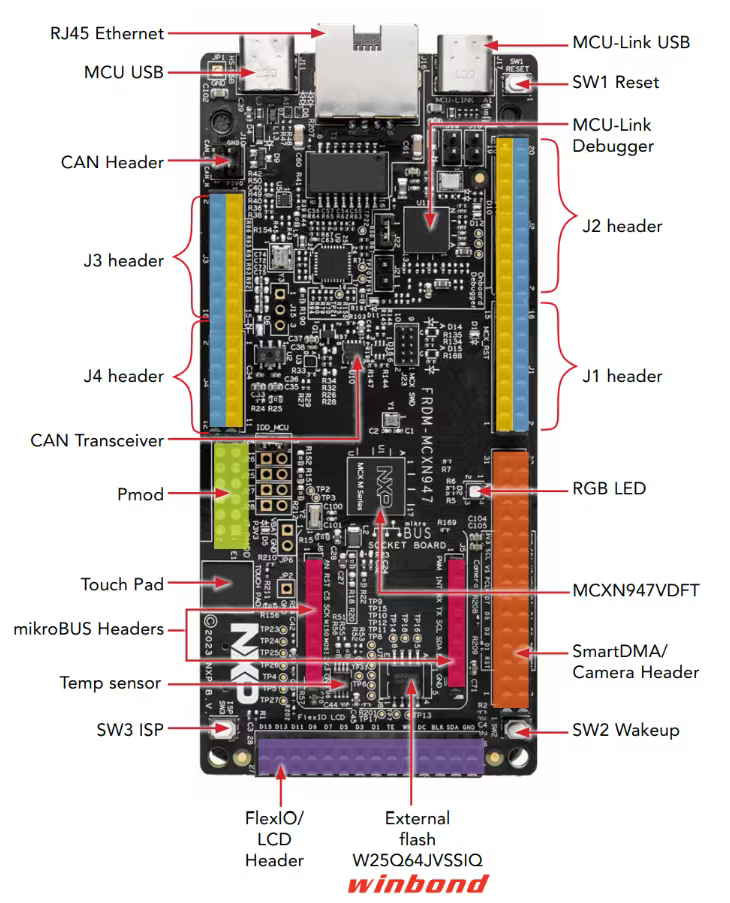
\includegraphics[width=0.65\textwidth]{obrazky-figures/frdm-mcxn947.png}
    
    \caption{Vývojová deska NXP FRDM-MCX947 \cite{nxp_FRDM_MCXN947_getting_started}}
    \label{fig:frdm-mcxn947}
\end{figure}

\subsubsection{NXP MCXN947}
Centrem mikrokontroléru MCXN947 jsou dvě jádra Arm® Cortex-M33 nové generace, pracující až na frekvenci 150 MHz. Jádro Cortex-M33 oproti předchozí generaci - Cortex-M3 je postaveno s novější instruční sadou ARMv8-M, která nabízí větší míru bezpečnosti v podobě TrustZone, jež umožňuje rozdělení paměťového prostoru na zabezpečenou (Secure World) a nezabezpečenou oblast (Non-Secure World). Dále jádro poskytuje možnost zvýšení výkonu pomocí integrovaného rozšíření DSP (Digital Signal Processor), které umožňuje efektivnější zpracování digitálních signálů a numerických výpočtů. \cite{nxp_MCX_Nx4x_Reference_Manual}

Z hlediska paměťových zdrojů nabízí MCXN947 512 KB paměti SRAM s podporou detekce a opravy chyb (Error Correction Code či zkráceně ECC). Pro zvýšení výkonu systému je čip vybaven několika typy rychlé paměti cache. Mikrokontrolér dále poskytuje 2 MB integrované flash paměti a pro programy s vyššími požadavky na úložiště je možné paměť rozšířit o dalších 8 MB prostřednictvím externí paměti typu flash připojené přes rozhraní Quad-SPI (QSPI). \cite{nxp_MCX_Nx4x_Reference_Manual}

Pro implementaci různorodých aplikací a variabilitu systému postavených na tomto čipu, MCXN947 nabízí širokou škálu periferií, které mohou být zajímavé z pohledu vývoje digitálního záznamníku. Mohou být například využity základní časovače v podobě CTIMER a CSTIMER, přes komunikační periferii LP\_FLEXCOMM, jež může být nastavena pro komunikační rozhraní I\textsuperscript{2}C, UART či SPI, nechybí ani podpora pro Ethernet a vysokorychlostní přenosy pomocí standardu USB 2.0 s Universal Serial Bus Full Speed Host and Device Controller (USBFS), který podporuje protokol OTG. Pro práci s paměťovými kartami je do čipu integrován Ultra Secured Digital Host Controller (uSDHC), který zprostředkovává komunikaci se SD, SDIO a MMC kartami. Čip MCXN947 také poskytuje tři instance A-D převodníku a taktéž tři komparátory. \cite{nxp_MCX_Nx4x_Reference_Manual}


\subsection{Raspberry PI - mikrokontrolér postaven na Linuxu}
Jednou z nejvýkonnějších možností pro implementaci digitálního záznamníku v podobě dedikovaného zařízení je využití mikroprocesorových platforem s operačním systémem Linux, přičemž nejznámějším zástupcem této kategorie je Raspberry Pi. Tato platforma spadá do kategorie jednodeskových počítačů (SBC – Single Board Computer), které kombinují výpočetní výkon a pružnost standardních počítačových systémů s rozhraními vhodnými pro práci s externími periferiemi.

Raspberry Pi je nízkonákladový minipočítač, de facto dnes už rodina počítačů, postavených na procesorech společnosti ARM, které podporují běh různých operačních systémů, nejčastěji Raspberry Pi OS. Raspberry Pi oproti klasickým mikrokontrolerům (MCU) poskytuje vyšší výpočetní výkon, taktéž i větší množství operační paměti (RAM) a podporuje také multitasking, umožňující běh více aplikací či procesů současně.

Raspberry Pi existuje v několika verzích, proto bude následný text věnován modelu Raspberry Pi Zero 2 W, který představuje rozumné parametry pro implementaci digitálního záznamníku v podobě dedikovaného zařízení. Model Zero 2 W je vybaven čtyřjádrovým procesorem Broadcom BCM2710A1 založeným na jádru ARM Cortex-A53 s taktem 1 GHz a disponuje 512 MB nízkoenergetické operační paměti SDRAM typu LPDDR2. Raspberry Pi Zero 2 W disponuje jedním USB portem typu micro-B, jenž podporuje režim OTG (On-The-Go) a umožňuje tak připojení externích zařízení, jako jsou USB flash disky či další periferie. Úložnou kapacitu zařízení lze jednoduše rozšířit díky přítomnosti slotu pro microSD kartu, která zároveň slouží jako primární úložiště operačního systému. Model Zero 2 W obsahuje také integrovaný bezdrátový komunikační modul podporující Wi-Fi standardu 802.11 b/g/n pracující v pásmu 2,4 GHz, díky kterému lze snadno implementovat digitální záznamník s podporou vzdáleného úložiště (viz. kapitola \ref{zapis_na_vzdalene_uloziste}).

\begin{figure}[h]
    \centering
    \includegraphics[width=0.85\textwidth]{obrazky-figures/raspberry_pi_zero_2w.png}
    
    \caption{Raspberry Pi Zero 2W vývody (pinout) \cite{arduino_shop_due}}
    \label{fig:raspberry-pi-zero-2w}
\end{figure}

Raspberry Pi tedy vypadá jako slibná varianta pro implementaci digitálního záznamníku, má však i své nevýhody. Hlavním omezením Raspberry Pi Zero 2 W je obecně nedostatek komunikačních periferií, platforma totiž disponuje pouze jedním modulem UART, jedním modulem SPI a jedním modulem I\textsuperscript{2}C. 
Tento omezený počet periferií může značně limitovat další rozšiřování zařízení o senzory či externí moduly. Například komplikace může nastat pouze při řešení vkládání časových razítek do záznamů, deska bohužel neobsahuje interní obvod reálného času, nabízí se  tedy využít jako referenční zdroj času, časovač (Timer) se softwarovým přerušením, druhou variantou je připojení záznamníku k síti a získat čas pomocí NTP (Network Time Protocol). Alternativním řešením se nabízí dokoupit externí obvod reálného času, to by znamenalo, že už by nebylo možné rozšířit zařízení o další periferie komunikující pomocí rozhraní I\textsuperscript{2}C, jelikož RTC moduly toto rozhraní většinou využívají, tedy sníží se možnost budoucích rozšíření.

\subsection{Shrnutí výběru platformy}
Jaká je tedy nejvhodnější platforma pro implementaci digitálního záznamníku ve formě dedikovaného zařízení? Vybral jsem FRDM-MCXN947 od společnosti NXP Semiconductors, jelikož poskytuje největší kompromis a nabízí nejvíce možností, z jakých komponent výsledný záznamník složit.

Alternativa Arduino Due, za svoji cenu za mě dostatečný poměr cena/výkon, jak je vidno v tabulce \ref{tab:board-comparison}. Maximální taktovací frekvence jádra je pouze 84 MHz, navíc to je postaveno na starší architektuře Cortex-M3. Kapacita flash paměti je oproti svým konkurentům za nižší cenu pouze 512 KB. V základu deska také neposkytuje možnost prostého rozšíření o externí uložiště jako je třeba micro SD karta, na které by mohly být získané záznamy uloženy. Také výběr, z jakého je možné vybrat řešení pro detekci ztráty napájení, je omezen.

Raspberry Pi Zero 2W naopak nabízí z vybraných možností velice dobrý poměr cena/výkon, obsahuje vysoce výkonný čip BCM2711 s taktem až 1.5 GHz a nabízí prostor, kde mohou být uloženy získané záznamy, a to konkrétně na micro SD kartě. Nicméně obtížněji by se řešilo vkládání časových značek a možná rozšíření v podobě doplňujících periferií.

\begin{table}[h]
    \centering
    \renewcommand{\arraystretch}{1.2}
    \begin{adjustbox}{max width=\textwidth} % Automatické přizpůsobení šířce stránky
    \begin{tabular}{|l|c|c|c|}
        \hline
        \textbf{Parametr / Platforma}   & \textbf{Arduino Due}  & \textbf{FRDM-MCXN947} & \textbf{Raspberry Pi} \\ 
        \hline
        \textbf{Typ čipu}               & ATSAM3X8E             & MCXN947               & BCM2711               \\ 
        \hline
        \textbf{Typ jádra}              & ARM Cortex-M3         & ARM Cortex-M33        & ARM Cortex-A53        \\ 
        \hline
        \textbf{Architektura jádra}     & 32-bit                & 32-bit                & 64-bit                \\ 
        \hline
        \textbf{Taktovací frekvence}    & 84 MHz                & 150 MHz               & 1.5 GHz               \\ 
        \hline
        \textbf{Operační paměť}         & 96 KB                 & 1 MB                  & Až 8 GB LPDDR4        \\ 
        \hline
        \textbf{Flash paměť}            & 512 KB                & 2 MB                  & MicroSD               \\ 
        \hline
        \textbf{Spotřeba }              & -                     & -                     & -                     \\ 
        \hline
        \textbf{Pořizovací cena}        & 2 058 kč (50,82€)                    & 593 Kč                & 459 Kč  \\ 
        \hline
    \end{tabular}
    \end{adjustbox}
    \caption{Porovnání vývojových desek Arduino Due, FRDM-MCXN947 a Raspberry Pi}
    \label{tab:board-comparison}
\end{table}
% ----------------------------------------------------
% DALSI NAZVY: Volba datového úložiště, Výběr externího uložiště pro záznam dat, Možnosti způsobu ukládání získaných dat
\section{Přístupy k ovládaní úložiště}
Obecný popis, proč je potřeba externí uložiště, že by se data mohla ukládat i v RAM paměti, ale že by tam moc dlouho nevydržela, 

\subsection{SDIO}

\subsection{SPI}

\subsection{Quad-SPI flash}


% ----------------------------------------------------
% DALSI NAZVY: Volba datového úložiště, Výběr externího uložiště pro záznam dat
\section{Možnosti správy dat - souborové systémy}
V předchozí části práce byla vybrána základní deska NXP FRDM-MCXN947 s mikrokontrolérem MCXN947, který bude sbírat data pomocí vstupní periferie, a tato data také zpracovávat pomocí jádra. Taktéž je vybráno externí úložiště, na které budou získaná data uložena, tím bude SD karta, konkrétněji SDHC karta. Data na tomto externím úložišti je třeba nějak organizovat, spravovat, aby mohla být v budoucnu nějakým způsobem interpretována a také popřípadě je třeba zajistit konzistenci a perzistenci uložených dat. K tomu účelu lze využít například souborový systém, databázový systém nebo data uchovávat v surovém (raw) formátu. Každý z těchto přístupů má svá specifika, nicméně data, která budou zaznamenávaná vyvíjeným záznamníkem, budou nestrukturovaná, rozhodl jsem se vybrat souborový systém. Souborový systém organizuje data přirozeně do souborů a složek a hodí se zejména pro již zmíněné ukládání nestrukturovaných dat. Pod pojmem nestrukturovaná data rozumíme taková data, která nejsou organizována jednotně v tabulkách (relacích) nebo databázových strukturách, ale mohou být ukládána do více typů souborů v různých formátech a umístěna do různorodých adresářových struktur. Tento přístup přináší výhodu, lze například získané záznamy hierarchicky členit, a zároveň umožňuje snadné přizpůsobení implementované logiky záznamníku pro ukládání i jiných typů dat. Díky tomu je záznamník obecněji využitelný pro různé typy záznamu. \cite{weka_structured_unstructured_data, virginia_tech_file_database_systems}

se  může proto existovat logika speciální pro danou aplikaci, jakou je třeba, anebo lze využít již vytvořené komponenty k tomu určené, mezi které patří i souborové systémy (File Systems).

Obecný popis, souborový systém je zodpovědný za organizaci, správu a přístup k datům na zvoleném úložném médiu.

\subsection{FATFS}
\label{fatfs}
Prvním z představených souborových systémů je FAT File System (FATFS), který je implementován v podobě lehké softwarové knihovny pro mikrokontroléry a vestavěné systémy implementující podporu souborového systému FAT/exFAT. FATFS se řadí mezi hierarchické souborové systémy založené na alokační tabulce souborů (File Allocation Table – FAT), ve kterých jsou data organizována do logických jednotek označovaných jako shluky (clusters). Každý soubor uložený na úložném médiu se tak skládá z jednoho nebo více těchto shluků, přičemž informace o jejich návaznosti jsou uloženy právě v alokační tabulce FAT. \cite{recoverit_fat_filesystem, elm_fat_filesystem_docs}

\begin{figure}[h]
    \centering
    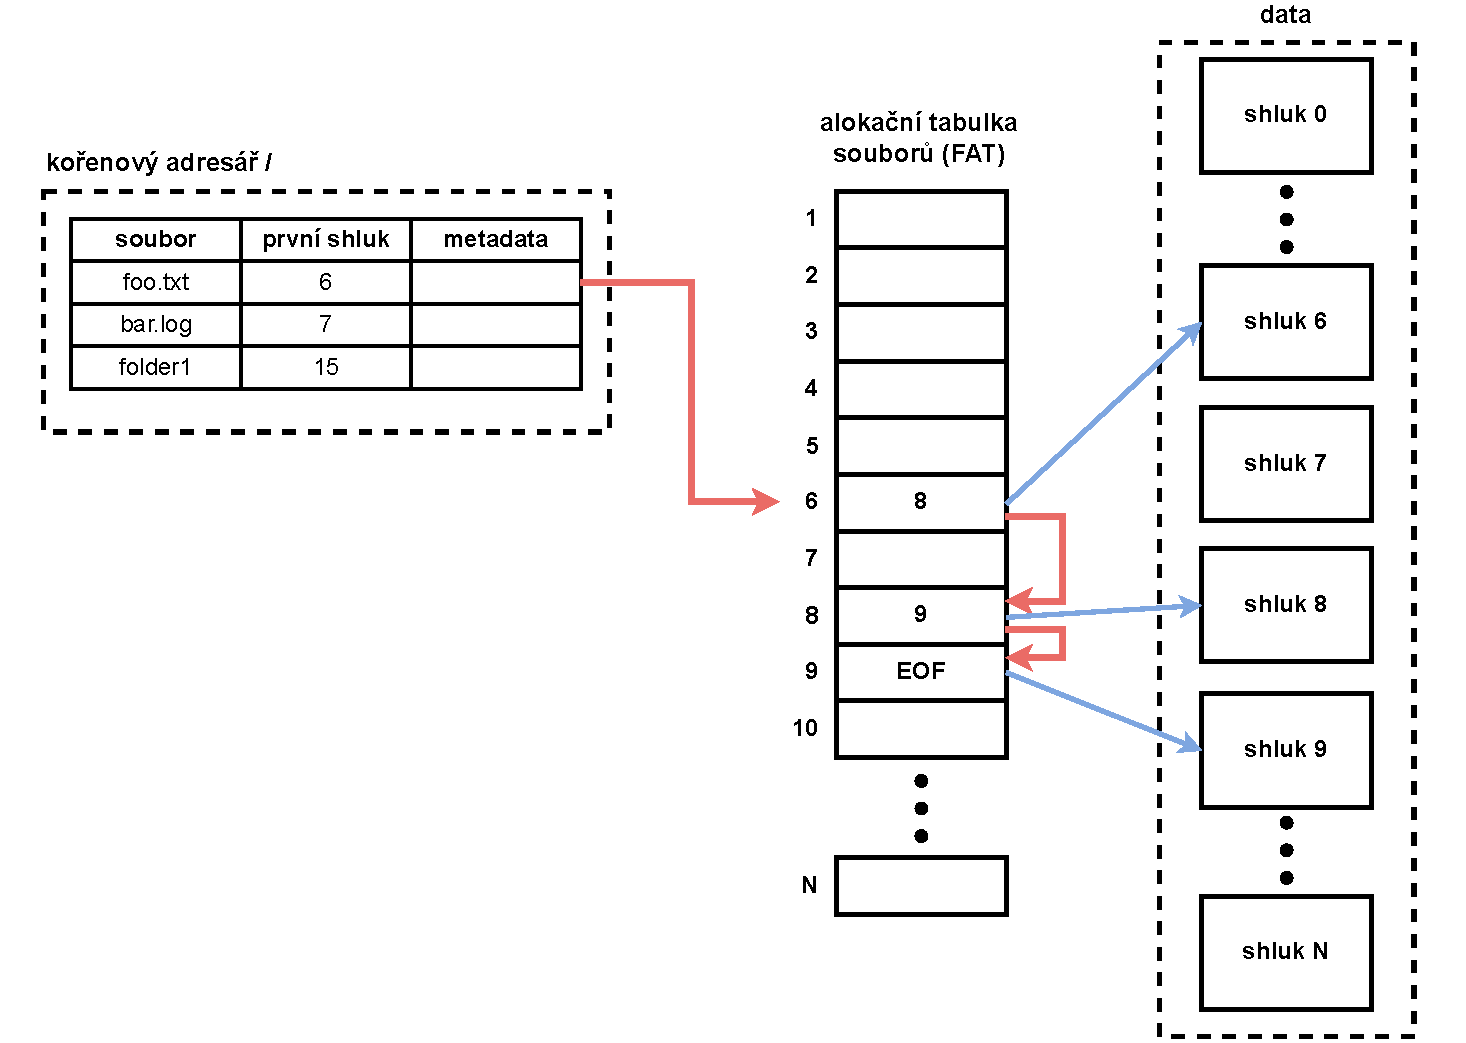
\includegraphics[width=0.80\textwidth]{obrazky-figures/fat_file_system-cz.pdf}
    
    \caption{Souborový systém s alokační tabulkou souborů \cite{recoverit_fat_filesystem}}
    \label{fig:fat-file-system-structure}
\end{figure}

Fyzické úložiště v systému FAT je rozděleno do několika oblastí, konkrétně do zaváděcího záznamu (Boot Record) ležícího v rezervované oblasti (Reserved Area), který obsahuje informace nutné pro inicializaci a načtení souborového systému, alokační tabulky FAT1 a FAT2, které spravují umístění jednotlivých shluků.  Za nimi se nachází oblast kořenového adresáře (Root Directory), ve které jsou umístěny záznamy o souborech a adresářích nejvyšší úrovně. Poslední část tvoří datová oblast (Data Area), kde jsou samotné soubory a podadresáře fyzicky uloženy.

\begin{figure}[h]
    \centering
    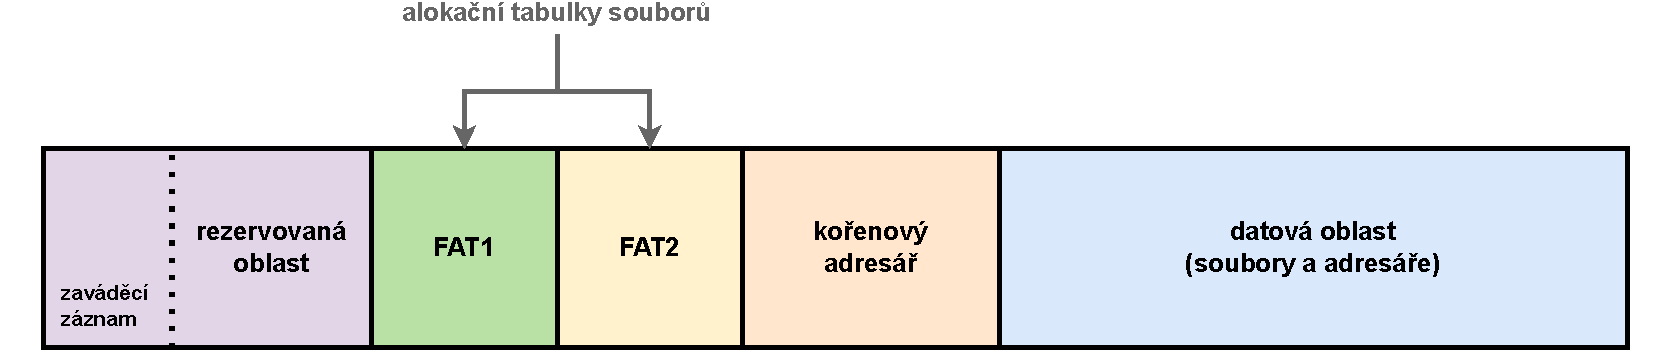
\includegraphics[width=1.00\textwidth]{obrazky-figures/fatfs_structure-cz.pdf}
    
    \caption{Oblasti souborového systému FAT \cite{recoverit_fat_filesystem}}
    \label{fig:fatfs-structure}
\end{figure}

% Jaky je rozdil mezi FAT32 a FATFS?
V dnešní době existuje několik variant systému FAT, mezi nejznámější patří FAT12, FAT16, FAT32 a exFAT. Pro úložná média typu SDHC karet se obvykle volí FAT32, neboť nižší varianty, jakou je třeba FAT16, omezují maximální kapacitu úložného média pouze na 4 GB, což je pro dnešní aplikace často nedostatečné. Z tohoto důvodu i dnešní implementace FATFS podporují 32bitovou LBA či 64bitovou LBA variantu, které podporují mnohem větší kapacitu uložišť. \cite{elm_fat_filesystem_app_note}

FATFS v současnosti představuje jeden z nejrozšířenějších souborových systémů pro použití ve vestavěných aplikacích, a to zejména díky své nízké paměťové náročnosti (nízký memory footprint) a snadné přenositelnosti mezi různými hardwarovými platformami. Významnou předností této knihovny je také široká možnost konfigurace, která umožňuje volby krátkých a dlouhých názvů souborů (Long File Name - LFN), navíc v různých formátech ANSI/OEM či Unicode. Pro velmi velká uložiště lze využít podporu exFAT s 64-bitovým adresováním bloků (LBA) a GPT (GUID Partition Table) pro práci s diskovými oddíly o velké kapacitě. FATFS také podporuje více fyzických jednotek či oddílů současně, variabilní velikost sektorů a různé kódové stránky. Knihovna rovněž obsahuje podporu pro volitelná rozhraní API, I/O buffering a režim pouze pro čtení. V případě použití v aplikaci běžící nad operačními systémy reálného času (RTOS) je výhodou této knihovny její bezpečnost, jelikož je garantována bezpečnost při práci ve vícevláknovém prostředí. \footnote{Knihovna FATFS je takzvaně Thread Safe.} \cite{elm_fat_filesystem_module}

% FAT is pretty bad on Flash devices because the low numbered sectors get rewritten frequently. Devices like USB sticks have wear levelling code, but if you're accessing raw hardware wear is a potential issue.

\subsection{LittleFS}
Alternativou k souborovému systému FATFS může být blokový (Block-Based) souborový systém LittleFS, který je podobně jako FATFS implementován ve formě odlehčené softwarové knihovny určené primárně pro vestavěné systémy a mikrokontroléry.  Tento systém byl vyvinut s ohledem na specifika flashových pamětí, aby se rovnoměrně rozdělil zápis na jednotlivé bloky a nebyly první bloky vytíženy více než ty s většími indexy.

\begin{figure}[h]
    \centering
    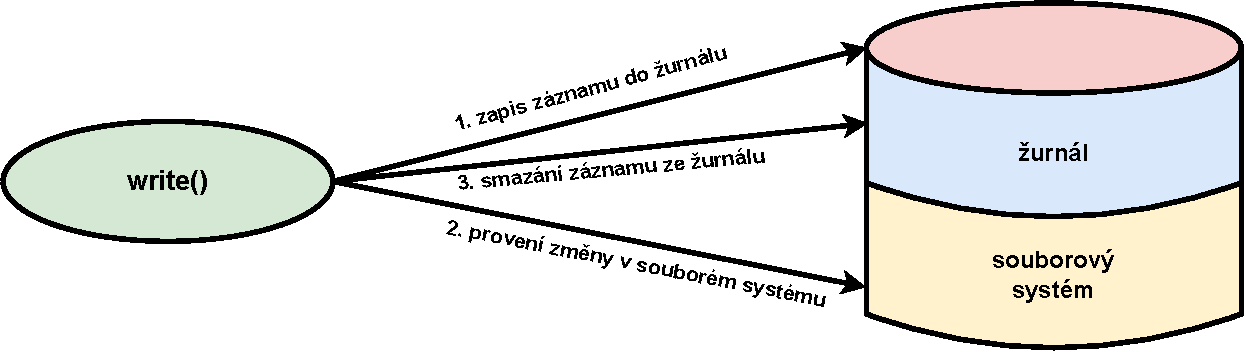
\includegraphics[width=0.95\textwidth]{obrazky-figures/journaling-cz.pdf}
    
    \caption{Průběh zápisu do souboru spravovaným žurnálovacím souborovým systémem \cite{architecture_and_design_of_the_linux_storage_stack}}
    \label{fig:journaling}
\end{figure}

% First we have the non-resilient, block based filesystems, such as FAT and ext2. These are the earliest filesystem designs and often the most simple. Here storage is divided into blocks, with each file being stored in a collection of blocks. Without modifications, these filesystems are not power-loss resilient, so updating a file is a simple as rewriting the blocks in place.
% https://github.com/littlefs-project/littlefs/blob/master/DESIGN.md

Souborový systém LittleFS využívá pokročilý mechanismus atomického zpracování známého z databázových systémů, kdy je každá operace buď kompletně dokončena, nebo v případě selhání či výpadku napájení zcela zrušena. K tomu je využit mechanismus žurnálování (journaling), který je využíván v pokročilých souborových systémech jako je ext3, XFS či ext4. Operace nad souborovým systémem jsou nejprve zaznamenány do speciální struktury (logu) před jejich fyzickým provedením. Pokud by došlo k selhání, jakým je například výpadek napájení, souborový systém se může spolehlivě vrátit do konzistentního stavu.

V souborovém systému LittleFS se k záznamu změn využívá technologie páry metadat (Metadata Pairs). Při každé operaci jsou měněna metadata souborového systému, přičemž tato metadata musí být aktualizována (měněna) atomicky. K změně jsou využity dvě speciální oblasti, označované jako metadata páry, které jsou opatřeny kontrolními součty (Checksum) a čísly revizí (Revision Count). Při každém zápisu se střídavě aktualizuje jeden ze dvou bloků metadat, přičemž druhý blok vždy uchovává předchozí konzistentní stav. Pokud by tedy došlo k selhání zápisu, souborový systém může jednoduše detekovat poškozený (Corrupted) stav a obnovit data z druhého, neporušeného bloku. \cite{nxp_the_design_of_the_little_filesystem}

Pro samotná data (Non-Meta Data) souborový systém LittleFS používá techniku Copy-on-Write (COW). Tato technika zajišťuje konzistenci dat tak, že při každém zápisu jsou aktuální (nová) data nejprve zapsána do volných bloků a teprve po úspěšném dokončení zápisu jsou bloky s neaktuálními/starými daty označeny jako volné. Pokud by tedy došlo během zápisu k chybě nebo výpadku napájení, systém se jednoduše vrátí k původním, neporušeným blokům, a tím zabrání ztrátě nebo poškození dat. \cite{nxp_the_design_of_the_little_filesystem}

Hlavními výhodami souborového systému LittleFS jsou tedy šetrnost k paměťovým médiím, nad kterými systém operuje, a také velmi nízká paměťová náročnost jak na velikost programového kódu ve flash paměti, tak na množství operační paměti RAM potřebné k jeho provozu. Dalším významným přínosem jsou již výše zmíněné pokročilé mechanismy známé z databázových systémů, zejména žurnálování a atomické operace, které umožňují zachovat souborový systém v konzistentním stavu i v případě neočekávaných selhání nebo výpadků napájení. \cite{nxp_the_design_of_the_little_filesystem}

Žurnálovací souborový systém LittleFS má ale také své nevýhody. Jednou z nejvýznamnějších je absence kompatibility při použití běžných paměťových médií, jakými jsou například SD či microSD karty, se standardními operačními systémy osobních počítačů, jakými jsou třeba Windows, Linux a MacOS. Data uložená pomocí LittleFS tak nejsou přímo čitelná na běžném počítači bez použití dodatečného softwarového nástroje (Wrapperu). \cite{cnx_software_little_fs}

\subsection{Chan FATFS}



% ----------------------------------------------------

\section{Výběr řízení přístupu k získaným datům}
\label{vyber_rizeni_pristupu_k_ziskanym_datum}
Důležitým prvkem digitálního záznamníku je také přístup k získaným datům, jak již víme, že data budou ukládána na SD kartu, respektive SDHC kartu a budou organizována a spravována souborovým systémem FatFs. Nutné je také připomenout, že jedním z požadavků na realizaci zařízení v této bakalářské práci je přístup k zaznamenaným datům bez nutnosti vyjmutí fyzického média. V úvahu připadávají varianty využívající USB či Ethernet, které vývojová deska NXP FRDM-MCXN947 nabízí, nicméně vzhledem k bezpečnostním restrikcím společnosti NXP není možné zařízení připojit k síti pomocí Ethernetového rozhraní. Tato skutečnost tedy omezuje dostupné možnosti přenosu dat pouze na komunikační protokoly nad rozhraním USB. 

% Mozna zde dopsat ze to uplne nezalezi na FS
% A file system defines how the files are organized in the storage media. The USB mass storage class specification does not require any particular file system to be used on conforming devices. Instead, it provides a simple interface to read and write sectors of data using the Small Computer System Interface (SCSI) transparent command set. As such, operating systems may treat the USB drive like a hard drive, and can format it with any file system they like. https://docs.silabs.com/protocol-usb/1.3.0/protocol-usb-msc-scsi/

\subsection{USB Mass Storage}
\label{usb_mass_storage}
První z možností pro zajištění přístupu k datům uloženým na SD kartě, respektive SDHC kartě, představuje použití standardu USB Mass Storage (MSC), vypracovaného v roce 1998 organizací USB-IF (USB Implementers Forum). Tento standard umožňuje, aby zařízení vystupovalo vůči hostitelskému systému jako standardní blokové zařízení (Block Device), host má tedy přímý přístup k celému uložišti. Protokol je dnes stále využíván a také podporován majoritní většinou moderních operačních systémů jako Microsoft Windows, operační systémy založené na Linuxu, tedy Ubuntu, Mint, Debian, ale také i Mac OS. Vyčíst data z SD karty či zapsat data na SD kartu lze tedy zvládnout téměř z kterékoliho osobního počítače.

Tento protokol rozlišuje dva komunikační prvky, prvním z nich je Mass Storage host, tedy zařízení, které aktivně řídí přístup k úložišti a provádí operace čtení a zápisu dat, tím je typicky osobní počítač nebo jiný hostitelský systém. Druhým prvkem je Mass Storage zařízení (Device), které je koncovým zařízením vystupující jako externí paměťové médium, tím může být například zmíněný Flash Disk či Hard Disk.

Z hlediska přenosových protokolů definuje USB Mass Storage dvě hlavní metody komunikace: Control/Bulk/Interrupt (CBI) a Bulk-Only Transport (BOT). CBI je přenosový protokol definovaný standardem USB 1.1, který kombinuje tři typy USB přenosů - řídicí (Control), blokové (Bulk) a přerušovací (Interrupt). Přenos se dále dělí na protokol přenosu dat, který využívá přenos přerušení, a protokol, který přenos přerušení nevyužívá. V současnosti nejrozšířenější metodou přenosu v rámci USB Mass Storage je transport pomocí BOT, v tomto režimu jsou data přenášena po blocích.
Součástí USB Mass Storage bývá také USB Floppy Interface (UFI), což je sada příkazů založená na SCSI-2 a SFF-8070 sadách příkazů, navržená pro jednoduchá bloková zařízení, původně určená pro USB disketové mechaniky (Floppy Disk), ale dnes běžně používaná pro základní interakci s jakýmkoliv typem Mass Storage zařízení. UFI definuje sadu příkazů pro čtení, zápis a správu paměťového média. \cite{usb_standard_ufi}

\begin{figure}[h]
    \centering
    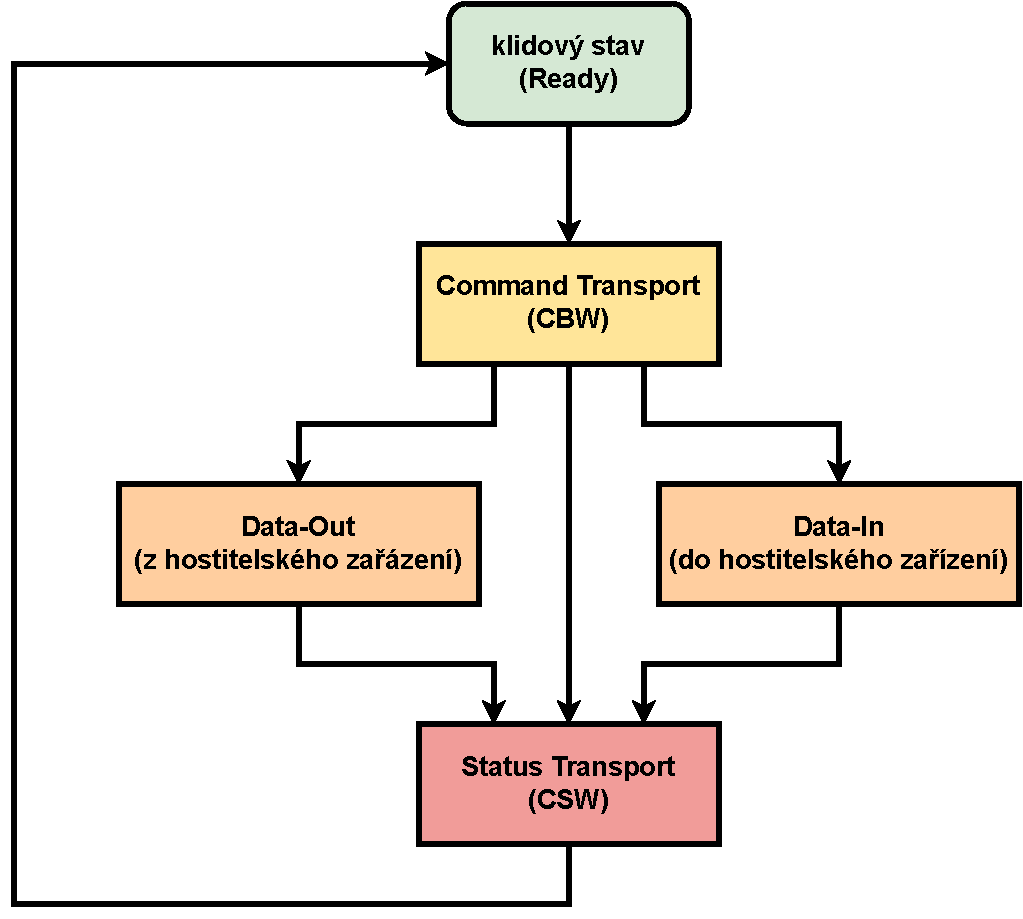
\includegraphics[width=0.65\textwidth]{obrazky-figures/mass_storage_protocol-cz.pdf}
    
    \caption{Stavový diagram USB Mass Storage protokolu \cite{silicon_labs_mass_storage_protocol}}
    \label{fig:mass-storage-protocol}
\end{figure}

Komunikace mezi hostitelem a zařízením v rámci protokolu Bulk-Only Transport (BOT) probíhá ve třech hlavních fázích, zajišťují řízený přenos příkazů, dat a zpětné vazby o provedení operace. První fází je přenos příkazu (Command Transport), během které host odešle zařízení požadavek na operaci v podobě struktury Command Block Wrapper (CBW). Tato struktura obsahuje informace o typu požadované operace (jakou je třeba inicializace, čtení, zápis), adresaci cílového sektoru na médiu a velikost přenášených dat. Pokud příkaz vyžaduje přenos dat, následuje druhá fáze - přenos dat (Data Transport). Data mohou být posílána ze zařízení do hostitele (například při čtení dat ze zařízení) nebo z hostitele do zařízení (například při zápisu na SD kartu). Přenos probíhá výhradně pomocí bulk přenosů. Poslední fází je Status Transport, v této fázi zařízení odešle zpět hostiteli strukturu CSW, která obsahuje informaci o výsledku provedené operace\footnote{v případě chyby může obsahovat další doplňující informace jako třeba množství nepřenesených dat (data residue)}. Ne všechny příkazy však vyžadují přenos dat (například příkazy pro kontrolu stavu zařízení), v těchto případech je fáze Data Transport vynechána a zařízení odesílá CSW ihned po přijetí CBW. \cite{silicon_labs_mass_storage_protocol}

% (Bulk-In/Bulk-Out). Poslední fází je Status Transport, v této fázi zařízení odešle zpět hostiteli strukturu CSW, která obsahuje informaci o výsledku provedené operace (úspěšné dokončení, chyba, množství nepřenesených dat – tzv. data residue)


\subsection{Media Transfer Protocol}
Media Transfer Protokol neboli zkráceně MTP je druhým významným protokolem umožňujícím přenos multimediálních dat mezi hostitelem a cílovým zařízením pomocí USB. MTP protokol byl navržen firmou Microsoft na základě protokolu Picture Transfer Protocol (PTP), se kterým je dodnes zpětně kompatibilní. MTP je od roku 2008 součástí USB standardu a od roku 2011 se stal standardem pro transfer souborů u zařízení využívajících operační systém Android. 

\begin{figure}[h]
    \centering
    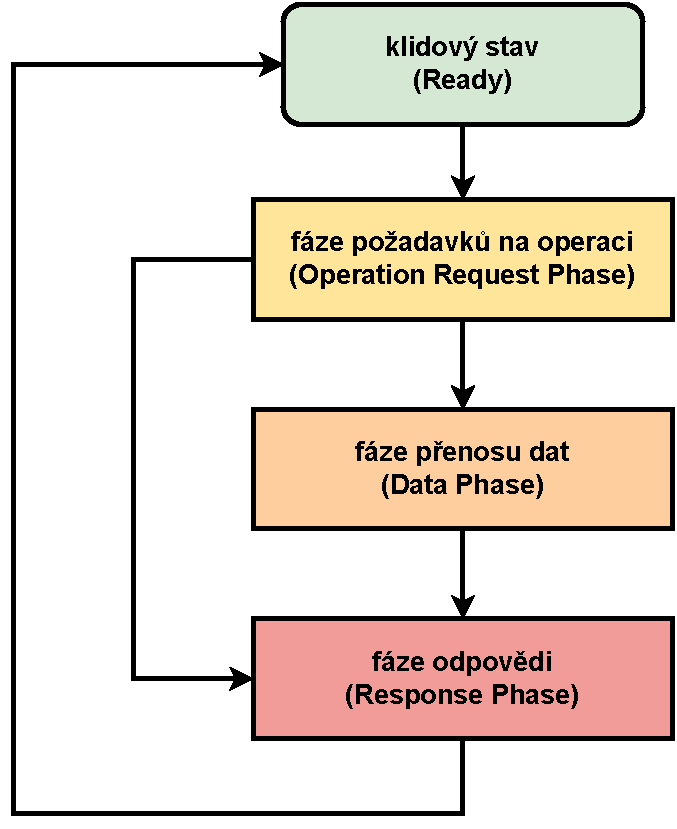
\includegraphics[width=0.50\textwidth]{obrazky-figures/mtp_phases-cz.pdf}
    
    \caption{Stavový diagram Media Transfer Protocol \cite{silicon_labs_mass_storage_protocol}}
    \label{fig:mtp-protocol}
\end{figure}

Komunikace probíhá ve formě transakcí, přičemž role komunikujících zařízení jsou iniciátor (Initiator) a odpovídající (Responder), zároveň je možné, aby si zařízení role mohly vyměnit. Transakce probíhají vždy ve třech fázích definovaných standardem, tou první je fáze požadavku na operaci (Operation Request Phase), kdy iniciátor vyšle požadavek na provedení určité operace. Následuje volitelná druhá fáze přenosu dat (Data Phase), ve které proběhne přenos dat, pokud to daná operace vyžaduje. Poslední je fáze odpovědi, ve které odpovídající odešle iniciátoru odpověď, ve které informuje o výsledku operace. Probíhající komunikace je vždy jednosměrná (Unidirectional), tedy v rámci jedné operace mohou data být pouze přenášena od iniciátora k odpovídajícímu či naopak, nikoliv však oběma směry současně. 


MTP na rozdíl od USB Mass Storage, kde je médium připojeno přímo jako blokové zařízení a hostitel má přímý přístup k souborovému systému, zde u MTP k tomu nedochází. Iniciátor tedy není zodpovědný za přímé operace se souborovým systémem, ale pouze zasílá žádosti o přenos nebo manipulaci se soubory. To znamená, že data zde nejsou interpretována připojeným zařízením (iniciátorem), ale interpretaci má na starosti odpovídající zařízení, a připojenému iniciátoru předává jen celé soubory. To přináší výhodu, že obě zařízení mohou přistupovat k datům současně (najednou). Naopak to, ale vytváří nové problémy - přes počítač nelze opravit poškozené soubory uložené na zařízení, v případě úpravy souboru je třeba nejprve soubor stáhnout do počítače, zde upravit a následně přenést zpět do zařízení.

\subsection{Human Interface Device}
Další možností pro zajištění přístupu k datům uloženým na SD kartě je využití standardu USB Human Interface Device (HID). Tento standard byl navržen původně společností Microsoft a posléze přijat jako součást USB specifikace za účelem unifikace komunikace s periferiemi, jako je klávesnice či počítačová myš. HID na rozdíl od USB Mass Storage (MSC) a Media Transfer Protocol (MTP), neslouží primárně pro práci se soubory nebo blokovými zařízeními, ale slouží jako univerzální protokol pro výměnu malých datových paketů (tzv. HID reportů). \cite{usb_standard_hid, silicon_labs_human_interface_device}

\begin{figure}[h]
    \centering
    
\includegraphics[width=1.00\textwidth]{obrazky-figures/hid_communication-cz.pdf}
    
    \caption{HID komunikace \cite{usb_standard_hid}}
    \label{fig:hid-communication}
\end{figure}

HID protokol definuje dvě základní role, prvním z nich je hostitelské zařízení (HID Host) a druhým je koncové zařízení (HID Device). Komunikace mezi těmito zařízeními probíhá primárně pomocí dvou typů přenosových kanálů (tzv. USB Pipe), které jsou pevně definovány standardem HID. Řídicí kanál (Control Pipe) slouží především pro inicializaci zařízení a konfiguraci přenosu dat. Přes tento kanál se přenáší tzv. HID Report Descriptor, což je struktura, která popisuje formát a význam jednotlivých HID reportů, které bude zařízení posílat hostitelskému zařízení. Řídicí kanál je taktéž využíván pro přístup ke zprávám o funkcích (Feature Reports), sloužící například k nastavování parametrů zařízení. Druhým z kanálů je přerušovací kanál (Interrupt Pipe), který slouží jako hlavní komunikační kanál pro pravidelný přenos datových rámců (reportů) mezi hostem a zařízením. Tento kanál je optimalizovaný pro malé datové pakety s nízkou latencí, typicky pro odesílání stavových informací, aktuálních měřených dat či událostí, jakým je třeba stisk tlačítka. Přerušovací přenosy probíhají periodicky, přičemž jejich frekvence je definována při enumeraci zařízení. \cite{usb_standard_hid, silicon_labs_human_interface_device}

% ----------------------------------------------------
\section{Výběr zdroje času}
\label{zdroje_casu}
Požadavkem na implementovaný digitální zaznamník  je také vkládání časových značek do záznamu, které budou využity pro následnou synchronizaci s druhým systémem. Způsobů, jak generovat časové značky, je mnoho, a je tedy nutné si na začátku stanovit základní požadavky, zda časové značky mohou být relativní (tedy například od času spuštění zařízení) či absolutní. Zároveň je však nutné při návrhu systému zvážit i další parametry, jakým je granularita časových značek, tedy časové rozlišení, s jakým budou události zaznamenávány, dále za zdroj času bude lokální nebo vzdálený. Tato kapitola představí některé ze způsobů, jak generovat časové značky, a dále rozebere jejich výhody a problémy, kterým konkrétní volby čelí. 

\subsection{Interní časovač}
Nejjednodušším způsobem pro generování časových značek je využít interní časovač, který je běžně dostupný na většině mikrokontrolérů. Interní časovač pracuje na základě přetečení čítače, který je taktován z hodinového signálu, jenž je generován interním oscilátorem nebo zvoleným hodinovým zdrojem mikrokontroléru. 

Schéma na následujícím obrázku \ref{fig:timer} znázorňuje základní strukturu interního časovače. Na vstupu se nachází multiplexer (Mux), pomocí kterého je třeba zvolit vhodný zdroj hodinového signálu, na základě kterého bude časovač reagovat, tedy inkrementovat. Tuto reakci můžeme dále ještě upravit pomocí děličky kmitočtu (Prescaler). Pomocí prescaleru lze snížit rychlost příchodu pulzů do čítače, a tím ovlivnit rychlost, s jakou časovač bude inkrementovat svou hodnotu. Na výstupu z prescaleru je napojen čítač (Module Counter), který s každým přijatým impulzem zvýší svou hodnotu o jedničku. Tento čítač je navíc svázán s modulo registrem (MOD), který definuje mezní hodnotu čítače. Jakmile čítač dosáhne hodnoty uložené v registru MOD, dojde k jeho přetečení (overflow), čítač se automaticky vynuluje\footnote{V nejjedošším případě je čítač vynulován, některé časovače, umožňují nastavit i jiné reakce, jakou je třeba dekrementace zpět na počáteční hodnotu.} a je vygenerován příznak přetečení (TOF - Timer Overflow Flag). Pokud je zároveň nastaven příznak TOIE (Timer Overflow Interrupt Enable), tak je do procesoru odeslán požadavek na vyvolání přerušení. V rámci obslužné rutiny tohoto přerušení je následně možné aktualizovat čítač časových značek a udržovat tak aktuální hodnotu pro následné doplnění do záznamů. 

\begin{figure}[h]
    \centering
    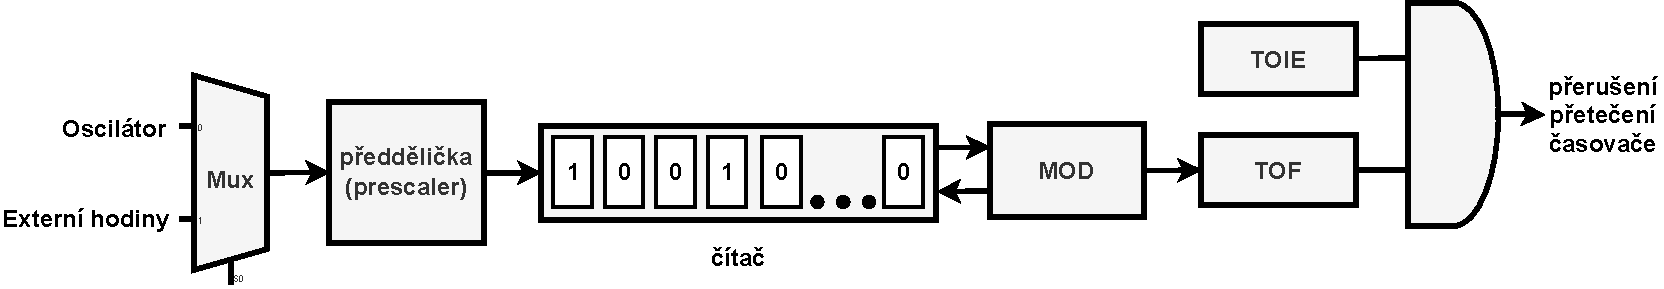
\includegraphics[width=1.00\textwidth]{obrazky-figures/timer-cz.pdf}
    
    \caption{Blokový diagram časovače}
    \label{fig:timer}
\end{figure}

Výhodou takového způsobu je výhoda v granulaci času, je možné přizpůsobit časové rozlišení. Časové rozlišení lze ovlivnit volbou hodinového zdroje, hodnotou děličky kmitočtu (prescaleru) a nastavením mezní hodnoty MOD. Lze tak snadno generovat přerušení s periodou i v řadě jednotek mikrosekund, sekundách až po výrazně delší časové úseky. V základní podobě poskytuje tento mechanismus měření relativního času, často od začátku běhu systému, pokud není použit doplňující prvek, který by umožňoval uchování či zjištění aktuálního času, jako je doplňující obvod reálného času nebo GPS modul. Právě skutečnost, že se jedná o relativní čas, přináší i určité výhody, odpadá totiž nutnost řešit komplexní problémy spojené s absolutním časem, jako jsou přechody mezi letním a zimním časem, nebo postupná odchylka interního časového základu od reálného času, která je přirozeným důsledkem výrobní tolerance oscilátorů a dalších časovacích prvků.

Takovýto způsob zproje času je sám o sobě pro záznam relativního času, často od začátku běhu systému, pokud není použit doplňující prvek, který by umožňoval uchování či zjištění aktuálního času, jako je doplňující obvod reálného času nebo GPS modul. Tím, že nepracuje s absolutním časem tj. skutečným časem, přináší další výhodu, a tou je, že není třeba řešit pokročilé problémy, které vznikají při práci s aktuálním časem, jako je nutnost řešit změny času z letního na zimní nebo třeba postupným rozjížděním času, se kterým zařízení pracuje od reálného času, jelikož časové prvky mají odchylku, jejíž význam bude časem narůstat.

Naopak mezi nevýhody použití interního časovače patří skutečnost, že takto získaný čas je pouze relativní, což v některých aplikacích nemusí být dostačující. Další nevýhodou je, že zpracování přerušení generovaných časovačem probíhá přímo v jádře systému, a tím odebírá výpočetní kapacitu, která by jinak mohla být věnována jiným úlohám. Platí přitom, že čím jemnější časové rozlišení je požadováno, tím vyšší je frekvence generovaných přerušení a tím větší je dopad na výpočetní výkon mikrokontroléru.

\subsection{Obvod reálného času}
\label{real_time_circuit}
Možné je také využít obvod reálného času (RTC - Real-Time Circuit), který je součástí většiny moderních mikrokontrolérů nebo dostupný jako samostatný externí integrovaný obvod. RTC je specializovaný časový modul navržený pro dlouhodobé uchování reálného času, tedy hodin, minut, sekund, ale často i datumu a dalších kalendářních informací.

Obvod reálného času je typicky taktován externím či integrovaným krystalem\footnote{Na obrázku \ref{fig:real-time-circuit} je krystal připojen pomocí vývodu X1 a X2 k RTC modulu.}, obvykle s rezonanční frekvencí 32,768 Hz. Tato hodnota není zvolena náhodně – odpovídá hodnotě $2^{15}$, tedy násobku dvou a umožňuje tak pomocí jednoduché děličky frekvence vydělit frekvenci na 1 Hz. Jeden kmit tak představuje jednu sekundu. Mnohé obvody reálného času také poskytují možnost připojení záložní baterie\footnote{Na obrázku \ref{fig:real-time-circuit} je baterie připojena pomocí vývodu VBAT a GND k RTC modulu.}, která slouží k udržení chodu interního časového obvodu i v případě, kdy je hlavní napájení zařízení odpojeno. Díky tomu může RTC kontinuálně uchovávat čas i po dlouhou dobu, kdy je zařízení neaktivní a není nutné čas nastavovat po každém startu zařízení. Jak již bylo zmíněno, RTC bývá často v podobě samostatných integrovaných obvodů nebo bývá integrován přímo v mikrokontroléru. Pro komunikaci mikrokontroléru s RTC jako samostatným integrovaným obvodem se obvykle využívá komunikační rozhraní I\textsuperscript{2}C, popřípadě SPI. Naopak k RTC integrovanému přímo do mikrokontroléru se přistupuje přímo prostřednictvím speciálních systémových registrů. \cite{jameco_choosing_right_real_time_clock_chip_or_module, yxc_role_of_32768_freq_in_the_circuit, medium_rtc}

\newpage

\begin{figure}[h]
    \centering
    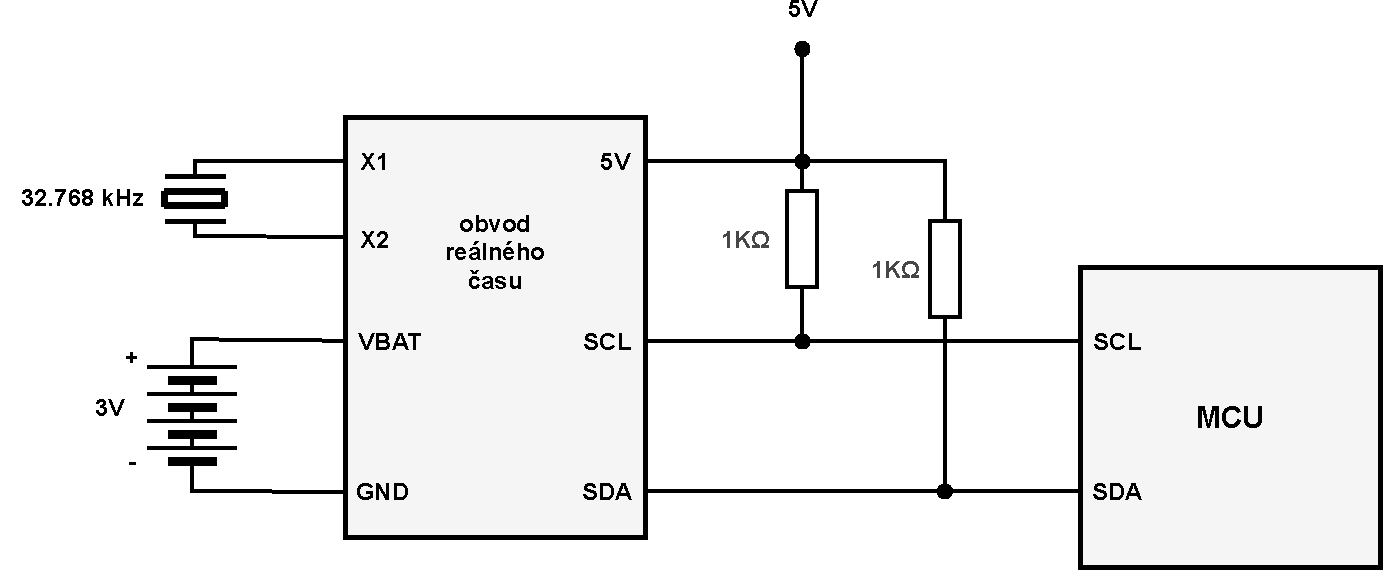
\includegraphics[width=1.00\textwidth]{obrazky-figures/real_time_circuit.pdf}
    
    \caption{Zapojení obvodu reálného času v podobě externího modulu připojeného k mikrokontroléru \cite{embed_journal_interfacing_rtc_with_microcontroler}}
    \label{fig:real-time-circuit}
\end{figure}

Obvod reálného času oproti běžnému časovači udržuje absolutní čas a dokáže jej udržovat dlouhodobě, a to i při přerušení napájení, pokud je tedy RTC vybaveno záložním napájením (například pomocí knoflíkové baterie).

Využití obvodu reálného času má, ale také své limitace či nevýhody. Zdrojem problémů může být například krystal, pomocí kterého je čas udržován, může například dojít k jeho poruše (například se krystal zastaví) či jeho rezonanční frekvence může být ovlivněna teplotními změnami. Může také nastat situace, kdy se vybije bateriový článek, poskytující napětí v době, kdy je hlavní napájení zařízení odpojeno, a je tak ztracena informace o aktuálním čase. Jedním z omezení je také minimální časové rozlišení, které je typicky nastaveno na sekundy. Mnoho standardních RTC modulů tak neumožňuje měřit a zaznamenávat čas s vyšší přesností, například v řádu milisekund či setin sekundy, což může být problémem u aplikací vyžadujících jemnější časovou osu. Také operování s absolutním časem vznikají specifické situace, jako například přechod mezi letním a zimním časem, změny časových pásem, navíc čas měřený obvodem reálného času se bude odchylovat od reálného času s narůstající dobou svého běhu, přičemž tato nepřesnost je dána konkrétním obvodem reálného času. \cite{jameco_choosing_right_real_time_clock_chip_or_module, embed_journal_interfacing_rtc_with_microcontroler, medium_rtc}

\subsection{Vzdálené zdroje času}
Další možností, jak získat časové značky, je využití vzdálených zdrojů času, které poskytují aktuální absolutní čas prostřednictvím komunikačního rozhraní. Takovými zdroji mohou být GPS satelity, NTP servery, rádiové stanice (například DCF77) a další specializované systémy. Přestože se tyto technologie mohou lišit ve způsobu přenosu a fyzikální povaze signálu (družicový, rádiový, síťový), sdílí některé principy pro určení aktuálního času. Standardně tyto systémy poskytují čas synchronizovaný vůči mezinárodnímu standardu UTC (Coordinated Universal Time) a zároveň pracují s hierarchickým modelem přesnosti označovaným jako stratum.

Koncept stratum slouží k vyjádření vzdálenosti daného časového zdroje od primárního referenčního času. Hodnotou stratum 0 jsou označeny primární zdroje času, takovými jsou například atomové hodiny. Následovné zdroje s hodnotou stratum 1 jsou přímo synchronizována se zařízeními s hodnotou stratum 0, přičemž další úrovně (stratum 2, 3 a vyšší) postupně navazují na předchozí zařízení s hodnotou stratum o jednu jednotku nižší.

\subsubsection{Globálního Polohovací Systém (GPS)}
Hodnotu stratum 0 mají například satelity globálního polohovacího systému (GPS), které právě obsahují atomové hodiny. Přesný čas satelitů je v systému GPS naprosto zásadní, neboť na jeho základě probíhá výpočet polohy přijímače. Bez znalosti velmi přesného času by totiž nebylo možné určit, za jak dlouhou dobu doputoval signál od satelitu k přijímači, a tím pádem by vznikaly chyby ve výpočtu vzdálenosti, respektive polohy.\footnote{Chyba jedné nanosekundy v tranzitním čase znaméná chybu 30cm ve zdálenosti.} GPS satelity tedy pravidelně vysílají rádiový signál (RF signál) obsahující identifikátor satelitu, hodinový signál (tj. čas) a části anmanachu obsahující například rovnici oběžné dráhy satelitu. Přijímač potřebuje tato data alespoň ze čtyř satelitů\footnote{GPS přijímač, může pro dopočitání využívá data i více než ze čtyř satelitů, aby se eliminovaly chyby vzniklé například z odchylek atovových hodin jednotlivých satelitů, či ze zanedbání faktu, že orbity satelitů nejsou zcela dokonalé kružnice.}, aby mohl dopočítat řešení čtyř rovnic o čtyřech neznámých, jehož součástí je i údaj o přesném čase pro přijímač. \cite{sparkfun_gps, time_theory_gps}

\begin{figure}[h]
    \centering
    \includegraphics[width=0.45\textwidth]{obrazky-figures/gps.png}
    
    \caption{Minimální nutná sestava čtyř GPS satelitů pro výpočet lokace a času přijímače \cite{time_theory_gps}}
    \label{fig:low-power-modes}
\end{figure}

Z pohledu přijímače má na starosti veškeré výpočty speciální GPS čipset, který integruje řadu funkcí potřebných pro správnou činnost systému. Kromě výpočtů spojených s určením polohy zpracovává i analogový rádiový signál přijatý anténou, provádí konverzi signálu do digitální podoby, spravuje řízení napájení a poskytuje rozhraní pro interakci s uživatelem. Rozdíly mezi čipovými sadami obvykle spočívají v rovnováze mezi spotřebou energie, časy akvizice a dostupností hardwaru. \cite{sparkfun_gps}

Jedna z nevýhod globálního polohovacího systému může nastat u zařízení využívaných v interiérech. Ve vnitřních prostorech může nastat problém se samotným průchodem signálu, moderní budovy často obsahují betonové stěny, kovové konstrukce, skla s metalizovanými vrstvami nebo střechy pokryté solárními panely, které představují překážky pro rádiový signál, a tak může být signál výrazně zeslaben nebo zcela pohlcen.

\subsubsection{Network Time Protocol (NTP)}
Další široce používanou technologií pro získání přesného času je síťový protokol NTP (Network Time Protocol). Tento protokol slouží k synchronizaci systémového času počítačových zařízení s časovými servery prostřednictvím sítí TCP/IP. NTP servery jsou organizovány do hierarchického systému vrstev (stratum), přičemž servery s nejnižším číslem (např. stratum 1) jsou přímo napojeny na referenční časové zdroje, jako jsou atomové hodiny nebo GPS přijímače (stratum 0). Servery na vyšších úrovních (např. stratum 2 a vyšší) získávají čas z těchto primárních zdrojů a zpřístupňují ho dále v síti.

Princip spočívá ve výměně časových značek mezi klientem a serverem. Klient odešle dotaz na NTP server ve chvíli $T_1$ a server tento dotaz přijme v čase $T_2$. Po zpracování server odešle odpověď v čase $T_3$, kterou klient přijme v čase $T_4$. Na základě těchto čtyř časových údajů lze vypočítat celkové síťové zpoždění $\delta$ a časový rozdíl (offset) $\theta$ mezi hodinami klienta a serveru. Zpoždění $\delta$ se určí jako:

\begin{equation}
    \delta = (T_4 - T_1) - (T_3 - T_2)
    \label{eq:ntp_delay}
\end{equation}
    

Zatímco rozdíl mezi klientským a serverovým časem čili offset ($\theta$), lze vypočítat dle vztahu:

\begin{equation}
    \theta = \frac{(T_2 - T_1) + (T_3 - T_4)}{2}
    \label{eq:ntp_offset}
\end{equation}

Získané hodnoty spoždění a rozdílu pak klientovi umožňují upravit systémový čas tak, aby co nejpřesněji odpovídal referenčnímu času. Protokol NTP navíc provádí více opakovaných měření a volí ty s nejnižším zpožděním, čímž zvyšuje stabilitu synchronizace i při kolísajícím síťovém připojení. \cite{sookocheff_ntp}

\begin{figure}[h]
    \centering
    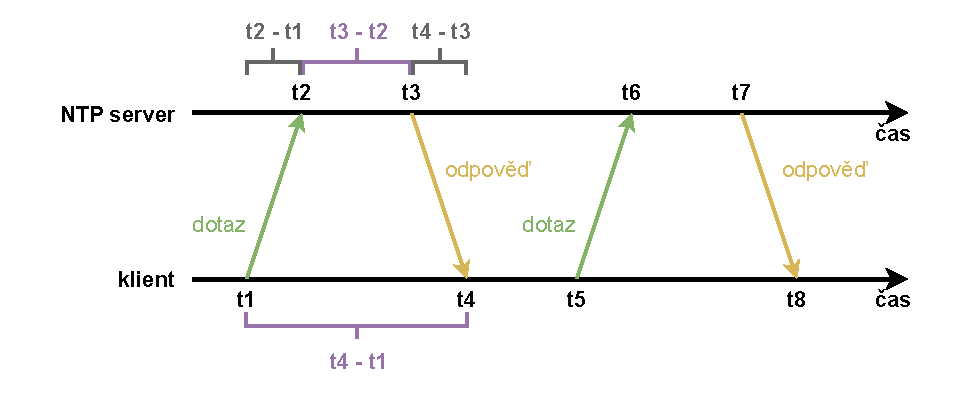
\includegraphics[width=0.95\textwidth]{obrazky-figures/network_time_protocol.pdf}
    
    \caption{Komunikace pomocí Network Time Protocol \cite{sookocheff_ntp}}
    \label{fig:network-time-protocol}
\end{figure}

NTP poskytuje přesný čas, nicméně také není vhodný pro každé vestavné zařízení vyžadující absolutní čas. Pro jeho fungování je nutná přítomnost TCP/IP zásobníku a zároveň aktivní síťové připojení k dostupnému NTP serveru. V prostředí, kde není možné garantovat trvalou konektivitu (například v mobilních, autonomních nebo izolovaných systémech), může být použití NTP omezené nebo zcela nevhodné. V takových případech je výhodnější spolehnout se na jiné zdroje času, jako je například GPS modul, nebo využít NTP pouze pro počáteční jednorázovou synchronizaci času při startu systému, kdy je připojení k síti dostupné.

% ----------------------------------------------------
\section{Výber přístupu řízení běhu aplikace}
Důležitou součástí, která bude určovat způsob, jakým bude výsledná aplikace implementována, je výběr způsobu řízení běhu aplikace. U aplikací vestavných zařízení se zpravidla rozhoduje mezi dvěma směry. Prvním z nich je implementace na holém železe, obvykle se pro tento způsob využívá anglický název bare-metal a druhou možností může být stavět program nad operačním systémem reálného času (Real-Time Operating System, zkráceně RTOS). Volba přístupu ovlivňuje výslednou architekturu. V následujících podkapitolách budou oba přístupy rozebrány, včetně jejich výhod a nevýhod. 


\subsection{Bare-Metal}
Bare-metal přístup znamená přímé řízení programu bez operačního systému, typicky s hlavní smyčkou (tzv. \emph{superloop}). Celý systém je dedikován pouze jedné aplikaci, která tak získává přímou kontrolu nad hardwarem. Program tedy přímo přistupuje k hardwarovým registrům mikrokontrolérů. 

Program se obvykle skládá ze dvou hlavních fází. První fází je inicializace, během které se nastavují systémové zdroje, konfiguruje se taktování, inicializují se periferie a případně se nastavují přerušení, nutné je podotknout, že tato fáze je provedena pouze jednou. Po dokončení inicializace přechází aplikace do hlavní smyčky, kde v nekonečném cyklu vykonává logiku programu, například zpracovává příchozí události a obsluhuje periferie. Řízení programu standardně probíhá sekvenčně, nicméně od tohoto sekvenčního provádění se odchýlí pouze tehdy, když dojde k události přerušení.

\begin{figure}[h]
    \centering
    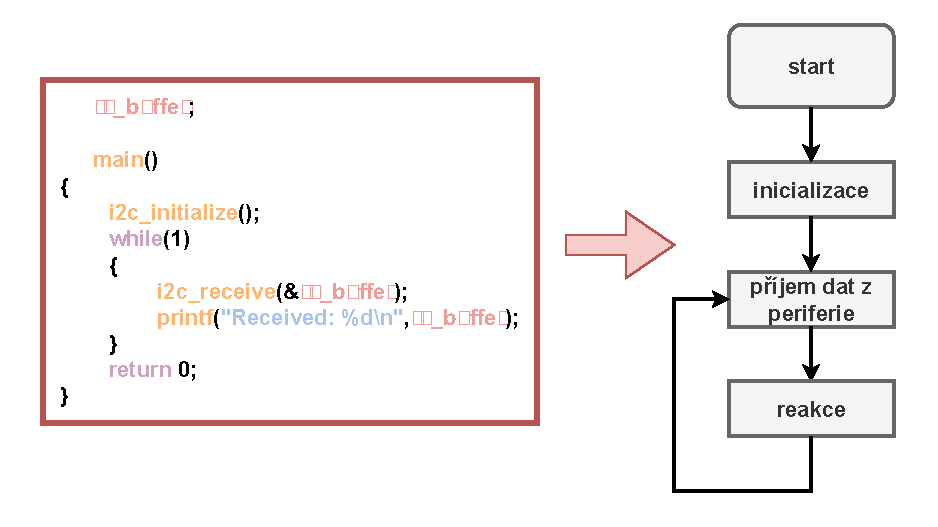
\includegraphics[width=1.00\textwidth]{obrazky-figures/bare_metal.pdf}
    
    \caption{Příklad vestavěnné aplikace využívající bare-metal přistup}
    \label{fig:bare-metal}
\end{figure}

% The bare-metal programming paradigm allows for maximum control and optimisation because the software is customised to the precise requirements of the ev embedded hardware. 
% https://medium.com/@ramjaju3737/concept-of-bare-metal-programming-in-embedded-systems-a8cd16422199
\newpage

Výhodou programování na bázi bare-metal je, že vestavné softwarové programy lze podrobně naplánovat pro konkrétní případ použití na co nejmenší úrovni, aniž by bylo nutné akceptovat režii navíc a možné chyby operačního systému. V optimálním případě tak vzniká řešení na míru, které spolehlivě plní úkoly a šetří zdroje. To má smysl vždy, pokud jsou úlohy, které mají být prováděny, zvládnutelné, takže lze zajistit co největší míru deterministického chování systému. \cite{sysgo_baremetal_vs_rtos}

Na druhou stranu, práce s holým systémem se vyskytují obtíže s zvládáním vysoké úrovně složitosti. Pokud se již tak nemalé projekty v průběhu implementační fáze nečekaně zvětší, například pokud přibudou nové funkce, které nebyly při předběžném plánování zohledněny, může být obtížné udržet si přehled. Tato obtíž může ještě narůst, pokud chybí hardwarová abstrakční vrstva nebo je navíc aplikace vyvíjená v assembleru a dokumentace k desce je nedostatečná, to může zkomplikovat vývoj i zkušeným programátorům. Nelze také opomenout, že manuální správa systémových prostředků, například ruční blokování prostředků pomocí semaforů, může být časově náročná a náchylná k chybám. \cite{sysgo_baremetal_vs_rtos}

% TODO: Zde to asi spis rozdelit na Baremetal vs. RTOS a pak uvest priklady jako FreeRTOS a ZephyrRTOS
\subsection{Operační systém reálného času}
Operační systém reálného času (RTOS) je typem počítačového operačního systému, který je navržen tak, aby byl malý a deterministický, tedy aby opakovaný vstup vedl ke stejnému výstupu. Tyto operační systémy se běžně používají ve vestavěných systémech, jako jsou lékařské přístroje a automobilové řídicí jednotky, které musí reagovat na vnější události v přísně omezeném čase. \cite{freertos_what_is_rtos}

RTOS podporuje multitasking, tedy schopnost spouštět více logických jednotek současně. Zmiňovanou nejmenší logickou jednotkou je obvykle vlákno (thread) nebo úloha (task)\footnote{Zde záleží na konkrétní implementaci RTOS například FreeRTOS používá úlohy, zatímco Zephyr RTOS pracuje s vlákny.}, které soutěží o čas procesoru a jsou vykonávána schedulerem. Na rozdíl od obecných operačních systémů, jako je Linux, které typicky využívají procesy (složené z jednoho či více vláken) izolované pomocí virtuální paměti, mnoho RTOS, zejména těch určených pro malé vestavné systémy, pracuje bez této vrstvy abstrakce. V takovém případě všechny úlohy sdílejí stejný fyzický adresní prostor a nejsou mezi sebou paměťově izolovány. Existují však i výkonnější RTOS, jako například Zephyr RTOS, které virtuální paměť a izolaci procesů podporují. \cite{freertos_what_is_rtos}

Plánovač je součástí jádra (kernelu), které představuje centrální komponentu RTOS a má na starosti správu běhu jednotlivých úloh (viz. obrázek \ref{fig:rtos-scheduling}) a přidělování procesorového času. Na rozdíl od jednoduchého sekvenčního provádění kódu v nekonečné smyčce mohou tyto úlohy běžet paralelně na základě priorit, časování a dalších parametrů. Kromě samotného plánování a přepínání mezi úlohami (tzv. přepínání kontextu) zajišťuje jádro také podporu pro synchronizaci a komunikaci mezi úlohami (např. semafory, fronty, mutexy), správu systémového času a obsluhu přerušení. Díky těmto funkcím umožňuje RTOS deterministické a přesně načasované vykonávání úloh.

\newpage

\begin{figure}[h]
    \centering
    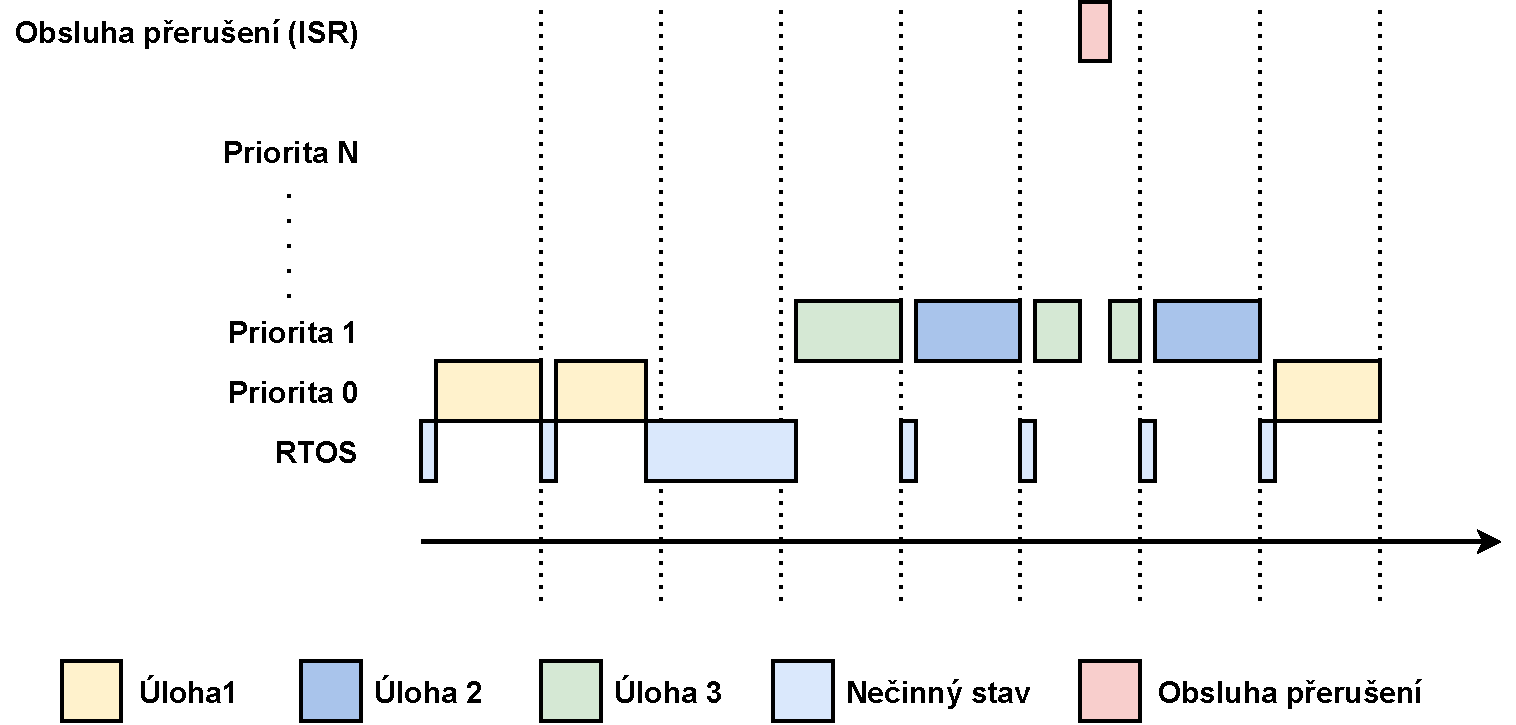
\includegraphics[width=0.90\textwidth]{obrazky-figures/rtos_scheduling.pdf}
    
    \caption{Graf znázorňující rozdělení výpočetního času, při řízení programu operačním systémem reálného času se schedulerem}
    \label{fig:rtos-scheduling}
\end{figure}

% RTOS je obvykle menší a lehčí než operační systém pro všeobecné použití, takže je vhodný pro zařízení s omezenou pamětí, výpočetní kapacitou a spotřebou energie.
Základními technickými výhodami RTOS jsou především deterministické chování, tedy schopnost reagovat na události ve striktně definovaném čase, a přesné řízení časování jednotlivých operací. To umožňuje systémům garantovat, že kritické úlohy budou vykonány ve stanovených časových limitech, bez ohledu na zátěž systému. Dále již byly nastíněny oblasti, ve kterých se operační systémy reálného času běžně uplatňují, mohou jimi být kritické systémy, jejichž selhání může mít katastrofální následky, například v robotice nebo v řídicích systémech letadel. Proto různé standardizované RTOS garantují vyšší bezpečnostní standardy a spolehlivější bezpečnostní funkce, například definované normami ISO 26262, DO-178C nebo IEC 61508.

Přestože operační systémy reálného času přinášejí řadu výhod, nelze opomenout ani jejich určitá omezení a nevýhody. Jedním z častých argumentů proti jejich použití je větší režie (overhead), která může snížit výkon a zvýšit paměťové nároky, čímž se zvyšují nároky na hardware. RTOS vnáší do systému složitost, která může ztížit jeho pochopení a ladění. Vývojáři musí být obeznámeni s rozhraním RTOS API a rozumět tomu, jak fungují úlohy, zdroje a komunikace mezi úlohami. Získání těchto znalostí může trvat delší dobu, což prodlužuje dobu vývoje a zvyšuje náklady. Použití RTOS může také zvýšit náklady na systém. Mnoho komerčních dodavatelů RTOS si účtuje licenční poplatky, které mohou být pro malé projekty nákladné.

\subsubsection{FreeRTOS}
Jednou z možností je FreeRTOS, což je open-source operační systém reálného času, který je podobný vývoji s bare-metal přístupem. FreeRTOS podporuje mnoho různých architektur a kompilátorů a je navržen tak, aby byl „malý, jednoduchý a snadno použitelný“. Jeho jádro tvoří v základu tři oblasti - správa úloh, komunikace a propojení s hardwarem. Správa úloh se stará o vytváření úloh, jak statických, tak dynamických, tak i jejich plánování a správu životního cyklu. Dále FreeRTOS poskytuje oblast zaměřenou na komunikaci mezi jednotlivými úlohami, k tomu slouží fronty (Queue). Úlohy a přerušení používají fronty k vzájemnému odesílání dat a k signalizaci použití kritických prostředků pomocí semaforů a mutexů. Poslední oblast slouží jako mezistupeň mezi hardwarově nezávislým jádrem FreeRTOS a hardwarově závislým kódem. \cite{the_architecture_of_open_source_applications}

Mezi hlavní výhody FreeRTOS patří jeho nízké nároky na systémové prostředky, což jej činí vhodným pro mikrokontroléry s omezenou pamětí a výpočetním výkonem. FreeRTOS poskytuje základní mechanismy pro plánování úloh, a to včetně prioritního plánovače s preempcí, který umožňuje přerušení aktuálně běžící úlohy ve prospěch jiné úlohy s vyšší prioritou. Velkou výhodou FreeRTOS je také jeho historie trvající přes 20 let, k dispozici je rozsáhlá dokumentace, příklady použití, mnoho výrobců, jako například NXP Semiconductors, poskytuje profesionální podporu. Z hlediska bezpečnosti FreeRTOS dodržuje přísný standard psaní kódu v souladu s normou MISRA-C, prochází statickou analýzou pomocí nástroje Coverity. Vybrané knihovny FreeRTOS byly navíc formálně ověřeny z hlediska paměťové bezpečnosti pomocí nástroje CBMC (C Bounded Model Checker). Bezpečnost systému byla rovněž potvrzena prostřednictvím certifikací SESIP™ Level 2 a PSA Certified Level 1, které vycházejí z rámce Common Criteria a hodnotí zabezpečení IoT platforem z hlediska architektury, implementace a odolnosti vůči útokům. \cite{freertos_security}

Přestože je FreeRTOS široce používán a oblíbený díky své jednoduchosti a nízké režii, nelze opomenout jeho omezení ve srovnání s robustnějšími RTOS, jakým je například Zephyr (viz. \ref{zephyr_rtos}). Nevýhodou může být omezená podpora knihoven a celkově nižší flexibilita. Není jednoduché jen tak přidat podporu na nový mikrokontrolér, jelikož portování je do značné míry jedinečné a velmi závislé na použitém procesoru a nástrojích. \cite{freertos_portability, freertos_vs_zephyr}

% Naproti tomu Zephyr RTOS má modulární, konfigurovatelný design a nabízí bohatou sadu subsystémů a knihoven. Má širokou hardwarovou podporu s více než 450 podporovanými deskami. 
% Konkrétní výhody a nevýhody FreeRTOS

\subsubsection{ZephyrRTOS}
\label{zephyr_rtos}
Zephyr RTOS je moderní open-source operační systém reálného času, který vznikl pod záštitou Linux Foundation a je aktivně vyvíjen komunitou i komerčními partnery. Zephyr je navržen jako modulární, bezpečný a škálovatelný systém, který lze přizpůsobit potřebám cílového zařízení pomocí nástroje Kconfig a popisu hardwaru ve formátu Devicetree. Typická aplikace postavená na operačním systému Zephyr je tvořena Zephyr jádrem, Zephyr moduly, vlastními moduly a aplikací, jak je možné vidět na obrázku \ref{fig:zephyr}. Zephyr moduly jsou poskytovány v rámci ekosystému operačního systému, zde patří například abstrakční vrstvy hardwaru poskytované různými výrobci čipů, jako je NXP Semiconductors, někdy je nutné si přidat vlastní moduly, těmi mohou být vlastní moduly a nakonec vlastní aplikace s logikou. Aplikaci je nutné nakonfigurovat, a jak již bylo zmíněno, k tomu se využívají nástroje Kconfig a DeviceTree. Nástroj Kconfig se používá ke konfiguraci jádra, subsystémů a softwarových knihoven a umožňuje  definovat, které části systému mají být zapnuty, jaké funkce mají být dostupné. Pro popis hardwarové struktury se Zephyr spoléhá na Devicetree, který určuje, jaké periferie jsou k dispozici, jak jsou propojeny. Popis periferií může být dále upraven nebo rozšířen pomocí overlay souborů (např. app.overlay), které přidávají nebo přepisují specifické uzly. Ze souborů Kconfig a Devicetree jsou při kompilaci vygenerovány hlavičkové soubory, které lze využít v aplikaci pro vestavěný systém. \cite{zephyr_doc_modules, embedded_summit_configure_zephyr}

\begin{figure}[h]
    \centering
    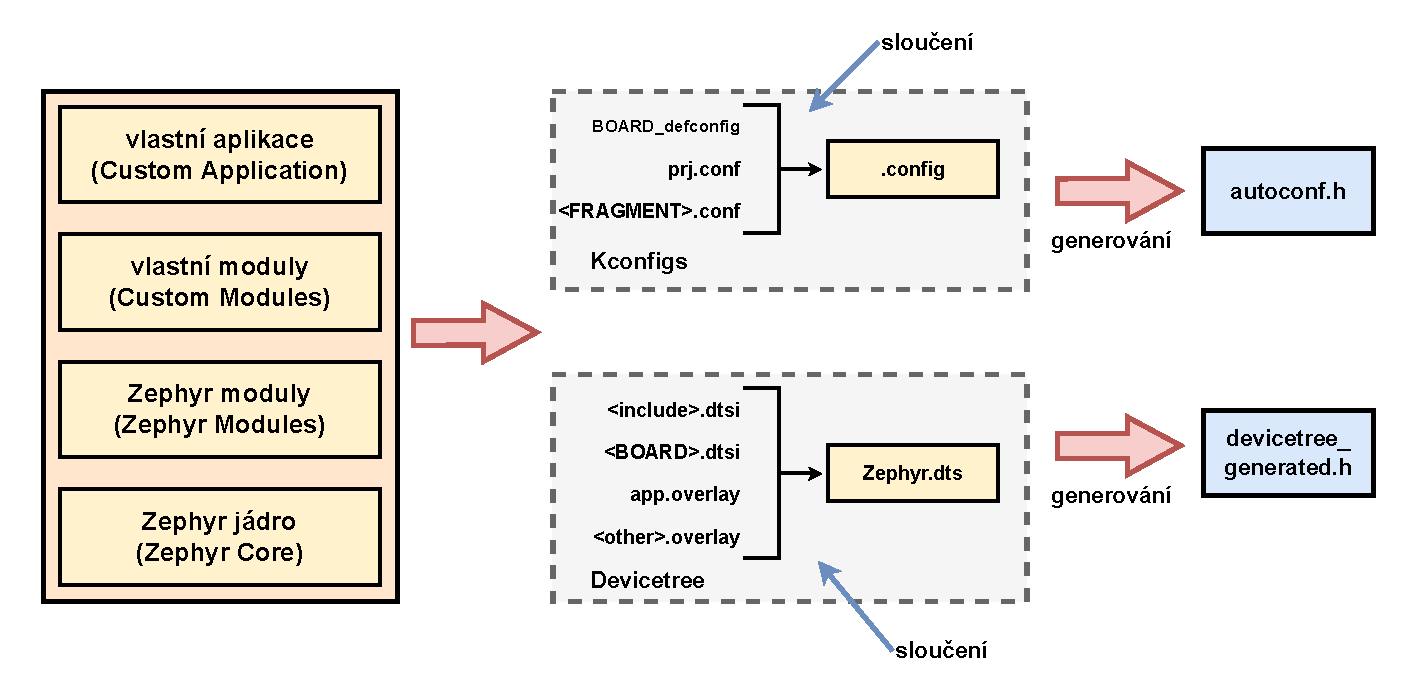
\includegraphics[width=1.00\textwidth]{obrazky-figures/zephyr.pdf}
    
    \caption{Přehled skladby projektu vyvíjeného s operačním systémem Zephyr \cite{embedded_summit_configure_zephyr}}
    \label{fig:zephyr}
\end{figure}

Mezi hlavní výhody operačního systému Zephyr patří jeho vysoká modularita a konfigurovatelnost, která umožňuje vývojářům sestavit jen ty části systému, které jejich aplikace skutečně potřebuje. Zephyr abstrahuje (mikro)jádro, HAL, middleware a komunikaci způsobem nezávislým na platformě, aplikační vrstva je tak oddělena od hardwarové vrstvy prostřednictvím abstrakcí v Devicetree a subsystémech jádra není aplikace pevně svázána s konkrétním mikrokontrolérem či deskou. Díky této abstrakci je možné aplikaci přenést na jinou desku s obdobným hardwarem zpravidla jen díky změnám v konfiguračních souborech. \cite{zephyr_advantages}

Na druhou stranu má Zephyr i své nevýhody, které mohou ovlivnit jeho vhodnost pro určité typy projektů. Vzhledem ke své komplexnosti může být učení se systému náročnější, a to zejména pro začínající vývojáře nebo pro jednodušší aplikace, kde je plně vybavený framework zbytečně robustní. I přesto, že je Zephyr dobře škálovatelný, základní velikost systému a spotřeba paměti jsou ve srovnání s minimalistickými RTOS, jako je FreeRTOS, vyšší. Další nevýhodou je, že vývojové prostředí Zephyru není na platformě Windows ještě plně dopracované. Přestože se podpora zlepšuje a základní funkcionalita je dostupná, není momentálně srovnatelná s prostředím na Linuxu, které je primární platformou pro vývoj aplikací s Zephyr operačním systémem. To je bohužel nevýhoda, jelikož v týmu, ve kterém pracují a který tento digitální záznamník bude využívat, je k dispozici výhradně systém Windows, což znesnadní budoucí vývoj případných rozšíření projektu. \cite{nabto_guide_zephyr_vs_freertos}


% ----------------------------------------------------
% Popis architektury na základě vybraných komponent. Popis blokového diagramu.

\section{Architektura systému digitálního záznamníku}
\label{architektura_systemu_digitalniho_zaznamniku}
Předchozí kapitoly představily vybrané komponenty, které lze využít k sestavení digitálního záznamníku v podobě dedikovaného zařízení. Rozhodl jsem se, že jako základ, čili platformu, zvolím vývojovou desku FRDM-MCXN947 od společnosti NXP Semiconductors (viz. \ref{nxp_frdm_mcxn947}), poskytující dostatečný výkon, paměťový prostor a periferie, které lze využít k realizaci záznamníku. Následující text bude popisovat architekturu jednotlivých komponent, architektura je následně graficky vizualizována na obrázku \ref{fig:system-architecture}.

Pro řízení činnosti záznamníku bude použit operační systém reálného času FreeRTOS, který umožní oddělit jednotlivé funkční části programu do samostatných paralelně běžících úloh. Architektura softwaru bude rozdělena do dvou hlavních úloh. Záznamová úloha bude zajišťovat průběžné získávání dat z UART periferie a jejich ukládání na paměťové médium. Komunikační úloha bude zodpovědná za zpřístupnění uložených dat prostřednictvím rozhraní USB ve standardu Mass Storage Class (MSC), čímž odpadá nutnost fyzického vyjímání paměťové karty ze zařízení. Pomocí tohoto přístupu lze dosáhnout vyšší modularity, přehlednosti a současného chodu obou činností bez vzájemného blokování.

Systém bude koncipován tak, aby v každém okamžiku byla aktivní vždy pouze jedna z hlavních úloh, což minimalizuje riziko konfliktu při přístupu k paměťovému médiu. Přepínání mezi úlohami bude řízeno detekcí připojení nebo odpojení USB rozhraní. V běžném režimu bude systém pracovat v záznamovém režimu a uchovávat příchozí data. Jakmile dojde k připojení zařízení k hostitelskému počítači, záznamová úloha se zastaví a aktivuje se komunikační úloha, která zpřístupní obsah úložiště jako běžný USB disk. Po odpojení USB se systém automaticky vrátí do režimu záznamu.

Po spuštění systému nejprve proběhne základní inicializace klíčových komponent, které budou aktivní po celou dobu běhu aplikace. V rámci této fáze se mimo jiné naváže komunikace s externím RTC modulem prostřednictvím sběrnice I\textsuperscript{2}C, ze kterého si mikrořadič přečte aktuální čas. Zjištěný čas bude následně uložen do interního RTC modulu, jenž je součástí samotného mikrořadiče. Práce s interním obvodem reálného času zrychlí přístup k systémovému času, jelikož další komunikace již nebude probíhat přes komunikační rozhraní I2C, ale přímo prostřednictvím registrů v rámci interní periferie.

Po úspěšné inicializaci bude následně jako výchozí a dominantní úloha spuštěna záznamová úloha, která zajistí příjem dat z externího zdroje. V rámci dané varianty digitálního záznamníku pro platformu NXP Semiconductors bude jako vstupní periferní rozhraní využit modul LP\_FLEXCOMM, nakonfigurovaný v režimu UART. Přijatá data budou dále zpracovávána a ukládána do paměťového úložiště s využitím postupů popsaných v kapitole~\ref{klicove_koncepty_digitalnich_zaznamniku}, přičemž bude kladen důraz na efektivní využití prostředků a minimalizaci ztráty dat i při vyšších přenosových rychlostech. Správu a organizaci dat v paměťovém médiu (SDHC karta) bude zajišťovat hierarchický souborový systém FATFS, který byl již představen v kapitole \ref{fatfs}.

Jakmile bude detekováno připojení k hostitelskému počítači, systém pomocí mechanismu USB OTG (On-The-Go) ověří, že došlo ke skutečnému připojení a navázání komunikace. V reakci na tuto událost se zařízení automaticky přepne do režimu Mass Storage, ve kterém bude vnitřní paměťové úložiště zpřístupněno jako běžný externí disk. Data tak budou přístupná bez nutnosti manipulovat se samotným zařízením nebo vyjímat paměťovou kartu.

\begin{figure}[h]
    \centering
    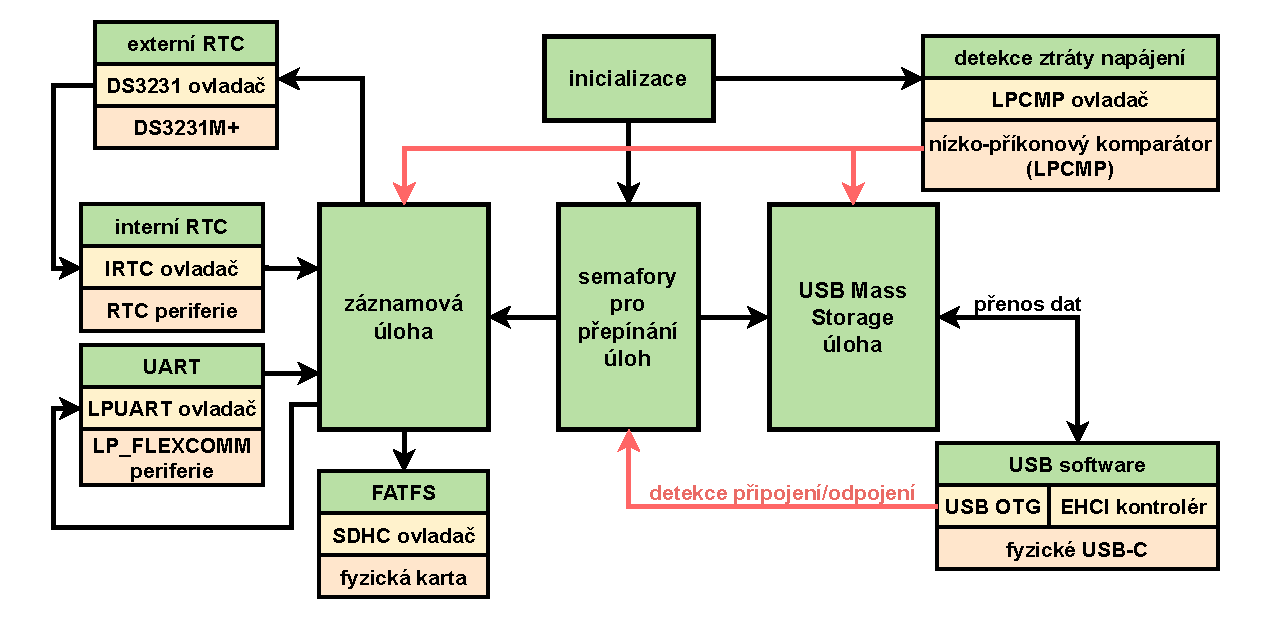
\includegraphics[width=1.00\textwidth]{obrazky-figures/system_architecture.pdf}
    
    \caption{Výsledná architektura digitálního záznamníku}
    \label{fig:system-architecture}
\end{figure}

Důležitou součástí návrhu systému je rovněž detekce ztráty napájecího napětí, která umožňuje včasnou reakci na neočekávané odpojení napájení. K tomuto účelu bude využita periferie LPCMP (Low-Power Comparator), která je součástí čipu na vývojové desce FRDM-MCXN947. Jakmile napájecí napětí poklesne pod stanovenou prahovou hodnotu, komparátor tento stav vyhodnotí a generuje událost, která informuje aplikační vrstvu o hrozícím výpadku. Od tohoto okamžiku je úkolem aplikace zajistit uložení všech rozpracovaných dat, která dosud nebyla zapsána do paměťového média, a také korektní uzavření otevřených souborů, aby bylo možné systém bezpečně ukončit a předejít ztrátě nebo poškození dat.


% ----------------------------------------------------

\section{Volitelné rozšíření}
\subsection{Měření teploty}

% ----------------------------------------------------

\subsection{Řešení problému synchronizace času}

% ----------------------------------------------------

\chapter{Realizace hardwaru}
\label{realizace_hardwaru}
Popis, co všechno je již na platformě FRDM MCXN947, z toho ti vyplyne, co všechno bude ještě muset nabízet expanzní deska.

\section{Základová deska}

\section{Expanzní deska}
Vybraná základová deska tedy neobsahuje všechny potřebné komponenty, které byly představeny v kapitole \ref{architektura_systemu_digitalniho_zaznamniku}. Pro zajištění kompletní funkcionality je proto nutné doplnit celý systém o expanzní desku plošných spojů, která umožní integraci všech klíčových externích komponent a rozšíří tak funkcionalitu základové desky. Tato kapitola představí realizovanou expanzní desku a její jednotlivé prvky.

\subsection{Zálohované napájení}
Důležitou součástí realizovaného digitálního záznamníku je zálohované napájení s detekcí ztráty napájecího napětí. Zálohované napájení lze realizovat několika způsoby, nejčastěji pomocí dobíjecí baterie (např. Li-Po nebo knoflíkového článku) nebo pomocí superkondenzátoru. Nejschůdnější variantou pro danou aplikaci se ukázal být superkondenzátor. Na rozdíl od baterií je schopen okamžitě dodat relativně vysoký vybíjecí proud (řádově stovky miliampérů), který byl naměřen při testování spotřeby pomocí zařízení Power Profiler Kit II od společnosti Nordic Semiconductors (viz. obrázek \ref{fig:power-consumption}), při kterém se ukázalo, že vstupní proud může dosáhnout hodnot až \SI{250}{\milli\ampere}. Běžné knoflíkové články nebo malé Li-Po baterie by v tomto ohledu nemusely zajistit dostatečný proud, nebo by vyžadovaly složitější obvody pro řízení nabíjení a ochranu. \cite{nordic_semi_ppk2}

% Zaroven musi byt jmennovite napeti vyssi z duvodu
Z tohoto důvodu bylo třeba vybrat superkondenzátor, který bude vyhovovat parametrům pro využití v digitálním záznamníku. Mezi takové parametry patří zejména kapacita, která určuje, jak dlouho je zařízení schopno fungovat po ztrátě napájení. Dále bylo nutné zohlednit jmenovité napětí, které musí být vyšší než maximální napájecí napětí systému, aby nedošlo k poškození součástky.\footnote{Běžně je doporučováno volit dvojnásobek či dokonce trojnásobek napětí při kterém bude kondenzátor operovat.} Dalším důležitým faktorem je ekvivalentní sériový odpor (ESR), jenž ovlivňuje schopnost superkondenzátoru dodávat vysoký proud bez výrazného poklesu napětí – čím nižší ESR, tím lépe je tedy kondenzátor schopen poskytovat vyšší proud. Vzhledem k omezenému prostoru na expanzní desce bylo zároveň nezbytné zohlednit fyzické rozměry kondenzátoru tak, aby jej bylo možné snadno integrovat a popřípadě umožnit, aby bylo možné využít dva kondenzátory paralelně, pro zvýšení spolehlivosti systému v případě selhání jednoho z kondenzátorů. \cite{cadence_capacitor_size}

\begin{figure}[h]
    \centering
    \includegraphics[width=0.80\textwidth]{obrazky-figures/power-consumption-2.png}
    
    \caption{Výsledek měření spotřeba implementovaného záznamníku pomocí Power Profiler Kit II 
    \cite{nordic_semi_ppk2}}
    \label{fig:power-consumption}
\end{figure}

Jako vhodný kondenzátor byl tedy vybrán model SCMR14G334SRBB0 od společnosti KYOCERA AVX s kapacitou \SI{0.33}{\farad}, jmenovitým napětím \SI{7.5}{\volt} při stejnosměrném proudu a nízkým ESR, které má konkrétní hodnotu \SI{450}{\milli\ohm}. Vzhledem k relativně nízké ceně této komponenty bylo třeba jej nejprve experimentálně ověřit v provizorním zapojení na nepájivém poli zobrazeném na následujícím obrázku \ref{fig:test-capacitors}. Kondenzátor byl v tomto testu nejprve nabíjen z laboratorního zdroje nastaveného na \SI{5}{\volt} – tedy napětí odpovídající reálným provozním podmínkám v cílovém zařízení. Po jeho odpojení byla sledována vybíjecí křivka sledována pomocí osciloskopu.

\begin{figure}[h]
    \centering
    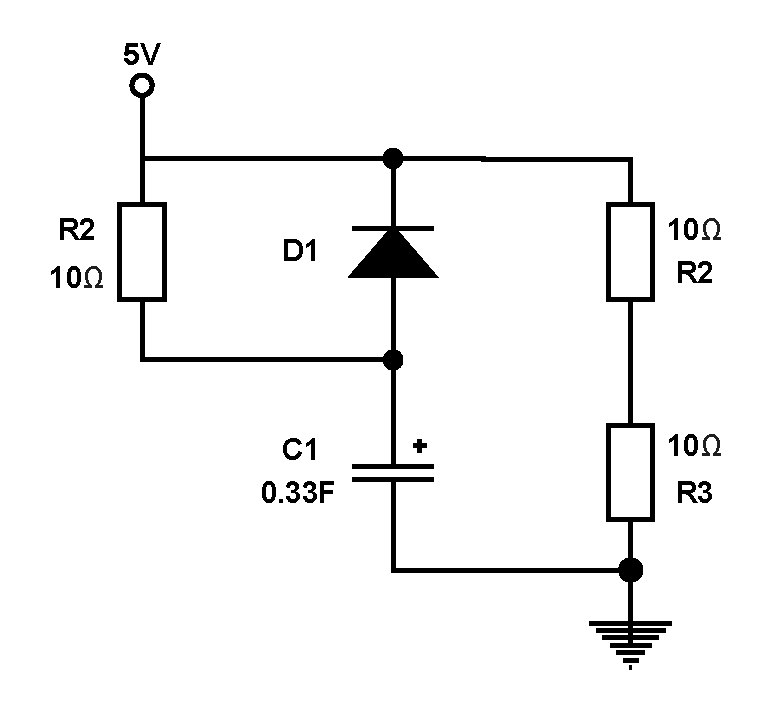
\includegraphics[width=0.440\textwidth]{obrazky-figures/test_capacitors.pdf}
    
    \caption{Obvod pro testování kondenzátoru}
    \label{fig:test-capacitors}
\end{figure}

Zapojení využívá Schottkyho diodu, na které vzniká úbytek napětí – konkrétně u použité součástky činí tento úbytek přibližně \SI{0.4}{\volt}. Aby bylo možné přesně vyhodnotit, jak dlouho dokáže záznamník fungovat při napájení ze superkondenzátoru, je třeba nejprve vysvětlit několik základních skutečností souvisejících s vývojovou deskou FRDM-MCXN947, která bude napájená z výše popsaného kondenzátoru. Vstupní napětí \SI{5}{\volt} jde přes LDO (Low-Dropout Regulator), které upravuje napětí na 3V3 zásobující čip. LDO však ke své funkci vyžaduje minimální rozdíl mezi vstupním a výstupním napětím, tzv. Dropout Voltage, při kterém je tento integrovaný obvod ještě schopen pracovat. Minimální vstupní napětí potřebné pro stabilní výstup 3.3V je dáno vztahem:

\[
V_{\text{LDO Min}} = V_{\text{LDO Out}} + V_{\text{Dropout}}
\]

V případě použitého stabilizátoru, který je využit na vývojové desce FRDM-MCXN947, je hodnota Dropout Voltage rovna \SI{0.2}{\volt} a minimální napětí, kterým tedy tato deska musí být napájena, činí \SI{3.5}{\volt}. Je tedy nutné sledovat napětí vybíjejícího se kondenzátoru v intervalu od \SI{4.6}{\volt} do \SI{3.5}{\volt}, které definuje časový interval, ve kterém je provoz vývojové desky stabilní.

Na následujícím obrázku \ref{fig:test-capacitors}, zachycujícím průběh napětí z výše zmíněného testu, zaznamenaného pomocí osciloskopu, ze kterého je patrné chování napájecího napětí v čase. Z naměřených dat vyplývá, že napětí na kondenzátoru zůstává v požadovaném funkčním rozsahu od \SI{4.6}{\volt} do \SI{3.5}{\volt} po dobu přibližně 1.3 sekundy. Pokud tedy dojde ke včasné detekci ztráty napájejícího napětí, může dojít k bezpečnému ukončení programu a korektnímu uložení všech potřebných dat, která jsou dočasně uložena ve volatilní paměti RAM, což potvrzuje vhodnost zvoleného superkondenzátoru pro danou aplikaci zálohovaného napájení.

\begin{figure}[h]
    \centering
    \includegraphics[width=1.00\textwidth]{obrazky-figures/capacitor-test-osciloscope.png}
    
    \caption{Obvod pro testování kondenzátoru}
    \label{fig:test-capacitors}
\end{figure}

Na následujícím obrázku \ref{fig:backup-power} je znázorněno výsledné schéma obvodu určeného k realizaci zálohovaného napájení včetně detekce ztráty hlavního napájecího napětí. Obvod zahrnuje zmíněnou Schottkyho diodu, která zabraňuje zpětnému toku proudu z kondenzátoru, a nabíjecí odpor s hodnotou $\SI{10}{\ohm}$, která byla zvolena tak, aby byl proud při nabíjení omezen na rozumnou úroveň, a zároveň aby nabíjení probíhalo v přiměřeném čase. Pro výpočet doby nabíjení je klíčovým parametrem časová konstanta~$\tau$, která je definována jako součin odporu~$R$ a kapacity~$C$:

\[
\tau = R \cdot C
\]

Součástí navrženého obvodu zálohovaného napájení je rovněž detekce ztráty napájecího napětí, jelikož je monitorována \SI{5}{\volt} větev, která překračuje maximální přípustné napětí pro přímé připojení na vstupy mikrokontroléru pracujícího s logikou \SI{3.3}{\volt}, je zapotřebí využít napěťový dělič, který upravuje napěťový signál, aby mohl být zpracován periferiemi pracujícími s digitálními signály, jako jsou GPIO, nebo analogovými periferiemi, jako je komparátor (CMP) či analogově-digitální převodník (ADC).

\begin{figure}[h]
    \centering
    \includegraphics[width=0.80\textwidth]{obrazky-figures/backup-power.png}
    
    \caption{Obvod pro detekci ztráty napájení a zálohované napájení}
    \label{fig:backup-power}
\end{figure}

\subsection{Obvod reálného času}
Již také bylo zmíněno, že pro uchovávání informace o čase a datu bude využit externí obvod reálného času. Tímto obvodem je konkrétně integrovaný obvod DS3231M+ od společnosti Analog Devices. Čip DS3231M+ patří mezi vysoce přesné RTC obvody obsahující integrovaný oscilátor s teplotně kompenzovaným krystalem (TCXO), který zajišťuje minimální odchylku chodu v řádu několika sekund za měsíc bez nutnosti externí kalibrace. Tato odchylka specifikována výrobcem činí \SI{\pm2} minut za rok v teplotním rozsahu od \SI{-40}{\degreeCelsius} do \SI{+85}{\degreeCelsius}.

Obvod reálného času s čipem DS3231M+ je integrován do expanzní desky plošných spojů (viz. obrázek \ref{fig:ds3231m+}) podle vzorového zapojení, jež bylo ukázáno v datasheetu k tomuto čipu. Pro komunikaci s tímto čipem se využívá jednoduché rozhraní I\textsuperscript{2}C s využitím dvou signálových linek, kterými jsou SDA (Serial Data Line) a SCL (Serial Clock Line). Linka SDA slouží k přenosu dat mezi mikrokontrolérem a RTC obvodem, zatímco linka SCL zajišťuje synchronizaci komunikace pomocí hodinového signálu. Kromě komunikačních linek je nutné k čipu připojit napájení. Pin V\textsubscript{CC} slouží pro napájení čipu v běžném provozu, kdy je deska aktivně napájena. Pro zachování správné funkce RTC i během výpadku napájení je k dispozici pin V\textsubscript{BAT}, který umožňuje připojení záložního zdroje, jakým může být například knoflíková baterie. Tento zdroj umožňuje čipu udržet běh vnitřního časovače a zachovat aktuální časovou informaci i během neaktivního stavu zařízení. 

Dále čip DS3231M+ obsahuje vývod 32KHZ, slouží jako výstup stabilního hodinového signálu o frekvenci 32 kHz. Tento pin má otevřený kolektor (open-drain) a vyžaduje připojení externího pull-up rezistoru, či může zůstat nezapojen. Multifunkční pin INT/SQW může pracovat buď jako výstup čtvercového signálu (square wave), nebo jako přerušovací výstup v případě shody časových registrů s nastaveným alarmem, který také není využíván digitálním záznamníkem, proto je připojen, taktéž jako 32KHZ přes pull-up rezistor k zemi. Posledním relevantním vývodem je RST, který slouží k resetování RTC obvodu. V návrhu expanzní desky je tento vývod připojen k jumperu, jehož sepnutím lze čip ručně resetovat.

\begin{figure}[h]
    \centering
    \includegraphics[width=0.80\textwidth]{obrazky-figures/ds3231m+.png}
    
    \caption{Obvod pro reálného času s čipem DS3231M+}
    \label{fig:ds3231m+}
\end{figure}

\subsection{GPS pro synchronizaci času}
Přestože integrovaný obvod reálného času DS3231M+ nabízí velmi dobrou dlouhodobou přesnost, stále jeho odchylka může činit až \SI{\pm2} minuty za rok. Mnoho aplikací vyžaduje ještě vyšší přesnost časové synchronizace, proto je expanzní deska připravena pro možnost připojení externího GPS modulu. Konkrétně se počítá s využitím modulu NEO-7M, který je schopen poskytovat přesné údaje o čase (UTC) díky synchronizaci s globálním navigačním systémem.

Modul NEO-7M obsahuje integrovaný přijímač, pasivní keramickou anténu a anténní zesilovač (nebo konektor pro připojení externí antény). Pokud jsou vyšší nároky na příjem signálu, je popřípadě možné pomocí SMA konektoru připojit aktivní anténu. Z následujícího obrázku~\ref{fig:neo-7m} je patrné, že GPS modul NEO-7M je možné připojit k mikrokontroléru pomocí vývodů TXD a RXD, které slouží pro komunikaci prostřednictvím sériového rozhraní UART. Prostřednictvím tohoto rozhraní poskytuje modul datový výstup ve formátu NMEA (National Marine Electronics Association), který je široce používaným standardem pro přenos informací z navigačních zařízení. Mezi nejčastěji přenášené údaje patří aktuální čas (UTC), zeměpisná šířka a délka, nadmořská výška, rychlost pohybu, směr pohybu, počet detekovaných satelitů, kvalita signálu a další navigační parametry. Modul NEO-7M poskytuje také speciální vývod PPS (Pulse Per Second), který generuje přesný časový impuls synchronizovaný s GPS systémem, který lze využít k synchronizaci ve vestavných systémech, například k časové korekci RTC nebo přesnému časovému značkování událostí. V rámci návrhu této expanzní desky však vývod PPS není připojen k mikrokontroléru, neboť pro potřeby této aplikace není jeho využití nezbytné.

\begin{figure}[h]
    \centering
    \includegraphics[width=0.70\textwidth]{obrazky-figures/neo-7m.png}
    
    \caption{Připojení GPS modulu NEO-7M}
    \label{fig:neo-7m}
\end{figure}

\section{Mechanická část}
Jak jsem měřil spotřebu, jak jsem spočítal hodnoty kondenzátorů 

\chapter{Přístup k realizaci obslužného firmware}
\label{softwarova_implementace}

\section{Záznamové vlákno}

\section{USB Mass Storage vlákno}

\begin{figure}[h]
    \centering
    \includegraphics[width=0.45\textwidth]{obrazky-figures/nxp_usb_device_application_structure.pdf}
    
    \caption{Vzorová struktura aplikace využívající NXP USB Stack \cite{silicon_labs_mass_storage_protocol}}
    \label{fig:usb-device-app-structure}
\end{figure}


\section{Signalizace stavu systému}

% ==================================================== 
\chapter{Testování systému}
\label{testovani_systemu}
Obecne proc je potreba testovat, jake jsou moznost testovani a validace vestavenych systemu

% ----------------------------------------------------

\section{Testování a validace}

\subsection{Funkcionální testování}
Popis skriptů pro automatické testování, popis výsledků, atd, ...

\subsection{Kontrola bezpečnosti kódu}
MISRA

% ----------------------------------------------------

\section{Limitace systému}
\label{limitace}

% ----------------------------------------------------

\section{Možná rozšíření záznamníku}
\label{mozne_rozsireni}

\chapter{Závěr}
\label{zaver}


%===============================================================================

% Pro kompilaci po částech (viz projekt.tex) nutno odkomentovat
%\end{document}

  \fi
  
  % Kompilace po částech (viz výše, nutno odkomentovat a zakomentovat input výše)
  % Compilation piecewise (see above, it is necessary to uncomment it and comment out input above)
  %\subfile{chapters/projekt-01-uvod-introduction}
  % ...
  %\subfile{chapters/projekt-05-zaver-conclusion}

  % Pouzita literatura / Bibliography
  % ----------------------------------------------
\ifslovak
  \makeatletter
  \def\@openbib@code{\addcontentsline{toc}{chapter}{Literatúra}}
  \makeatother
  \bibliographystyle{bib-styles/Pysny/skplain}
\else
  \ifczech
    \makeatletter
    \def\@openbib@code{\addcontentsline{toc}{chapter}{Literatura}}
    \makeatother
    \bibliographystyle{bib-styles/Pysny/czplain}
  \else 
    \makeatletter
    \def\@openbib@code{\addcontentsline{toc}{chapter}{Bibliography}}
    \makeatother
    \bibliographystyle{bib-styles/Pysny/enplain}
  %  \bibliographystyle{alpha}
  \fi
\fi
  \begin{flushleft}
  \bibliography{projekt-20-literatura-bibliography}
  \end{flushleft}

  % vynechani stranky v oboustrannem rezimu
  % Skip the page in the two-sided mode
  \iftwoside
    \cleardoublepage
  \fi

  % Prilohy / Appendices
  % ---------------------------------------------
  \appendix
\ifczech
  \renewcommand{\appendixpagename}{Přílohy}
  \renewcommand{\appendixtocname}{Přílohy}
  \renewcommand{\appendixname}{Příloha}
\fi
\ifslovak
  \renewcommand{\appendixpagename}{Prílohy}
  \renewcommand{\appendixtocname}{Prílohy}
  \renewcommand{\appendixname}{Príloha}
\fi
%  \appendixpage

% vynechani stranky v oboustrannem rezimu
% Skip the page in the two-sided mode
%\iftwoside
%  \cleardoublepage
%\fi
  
\ifslovak
%  \section*{Zoznam príloh}
%  \addcontentsline{toc}{section}{Zoznam príloh}
\else
  \ifczech
%    \section*{Seznam příloh}
%    \addcontentsline{toc}{section}{Seznam příloh}
  \else
%    \section*{List of Appendices}
%    \addcontentsline{toc}{section}{List of Appendices}
  \fi
\fi
  \startcontents[chapters]
  \setlength{\parskip}{0pt} 
  % seznam příloh / list of appendices
  % \printcontents[chapters]{l}{0}{\setcounter{tocdepth}{2}}
  
  \ifODSAZ
    \setlength{\parskip}{0.5\bigskipamount}
  \else
    \setlength{\parskip}{0pt}
  \fi
  
  % vynechani stranky v oboustrannem rezimu
  \iftwoside
    \cleardoublepage
  \fi
  
  % Přílohy / Appendices
  \ifenglish
    % This file should be replaced with your file with an appendices (headings below are examples only)

% For compilation piecewise (see projekt.tex), it is necessary to uncomment it and change
%\documentclass[../projekt.tex]{subfiles}
%\begin{document}

% Placing of table of contents of the memory media here should be consulted with a supervisor
%\chapter{Contents of the included storage media}

%\chapter{Manual}

%\chapter{Configuration file}

%\chapter{Scheme of RelaxNG configuration file}

%\chapter{Poster}

\chapter{How to use this template}
\label{jak}

This chapter describes individual parts of the template, followed by a brief instructions on how to use it. If you have any questions, comments etc, feel free to email them to \texttt{sablona@fit.vutbr.cz}.

\section*{Template parts description}

Once you extract the template, you will find the following files and directories:
\begin{DESCRIPTION}
  \item [bib-styles] Literature styles (see below). 
  \item [obrazky-figures] Directory for your images. Currently contains \texttt{placeholder.pdf} (a.k.a TODO image -- see below) and image keep-calm.png to demonstrate inserting raster images (you don't submit these images with your thesis). It is advised to use shorter directory name, so that it is only in your chosen language.
  \item [template-fig] Template images (BUT logo).
  \item [fitthesis.cls] Template (design definition).
  \item [Makefile] Makefile used to compile the project, count standard pages etc. (see below).
  \item [projekt-01-kapitoly-chapters-en.tex] File for Your text (replace it's contents).
  \item [projekt-20-literatura-bibliography.bib] Reference list (see below).
  \item [projekt-30-prilohy-appendices-en.tex] File for your appendices (replace it's contents).
  \item [projekt.tex] Main project file -- definitions of formal parts.
\end{DESCRIPTION}

The style of literature in the template is from Ing. Radek Pyšný \cite{Pysny}, whose work was improved by prof. Adam Herout, dr. Jaroslav Dytrych and Mr. Karel Hanák to comply with the norm and support all frequently used types of citations. Its documentation can be found in the appendix

Aside from compilation to PDF, the Makefile also offers additional functions:
\begin{itemize}
  \item rename files (see below),
  \item count standard pages,
  \item run a wave that adds unbreakable spaces,
  \item compress (zip) the result, ready to be sent to your supervisor and checked (make sure that all the files you've added are included, if not, add them manually).
\end{itemize}

Keep in mind that the wave is not perfect. You always need to check whether or not there is something inappropriate at the end of a line manually -- see Online language handbook\footnote{Internetová jazyková příručka \url{http://prirucka.ujc.cas.cz/?id=880}}.

Similar rules apply also in English - see eg. article Run Ragged\footnote{Run Ragged\url{https://24ways.org/2013/run-ragged/}}, according to which there should be no prepositions, dash or short words (2--3 letters) at the end of the lines, the two lines following each other should not end with a comma and line break should not be also in the phrases from 2-3 words.

\paragraph {Pay attention to page numbering!} If the table of contents is 2 pages long and the second page contains only \uv{Enclosures} and \uv{List of enclosures} (but there is no enclosure), the page numbering is changed by 1 (table of contents and contents \uv{mismatch}). The same thing happens if the second or third page contains only \uv{References} and there's a chance that this can occur in other situations too. There are multiple solutions to this (from editing the table of contents, setting the page counter all the way to more sophisticated methods). \textbf{Check the page numbering before you submit your thesis!}

\section*{Recommendations for working with the template}

\begin{enumerate}
  \item \textbf{Make sure you have the latest version of template.} If you have a template from last year, there should be a newer version (updated information, fixed errors etc.) available at the faculty or study advisor web pages.  
  \item \textbf{Choose a language}, that you want to use for your technical report (czech, slovak or english) and consult your supervisor about your choice (unless it was agreed upon in advance). If your language of choice is not czech, set the respective template parameter in file projekt.tex (e.g.: \verb|document|\verb|class[english]{fitthesis}| and translate the declaration and acknowledgement to english or slovak).
  \item \textbf{Rename the files.} When you extract the files, there should be a file named projekt.tex. If you compile it, it will create a PDF with technical report named projekt.pdf. If multiple students send their supervisor projekt.pdf to have it checked, they have to rename them. For that reason, it is advised to rename the file so that it contains your login and (if needed, abbreviated) work topic. Avoid using spaces, diacritic and special symbols. An appropriate name for your file can look like this: \uv{xlogin00-Cleaning-and-extraction-of-text.tex}. You can use the included Makefile to rename it: 
\begin{verbatim}
make rename NAME=xlogin00-Cleaning-and-extraction-of-text
\end{verbatim}
  \item Fill in the required information in file, that was originally named projekt.tex, that means type, year (of submission), thesis title, author's name, department (according to specification), supervisor's titles and name, abstract, keywords and other formal requirements.
  \item Replace the contents of thesis chapters, references and enclosures files with the contents of your technical report. Individual enclosures or thesis chapters can be saved to separate files -- if you choose this approach, it is advised to comply with the file naming convention, and the number will be followed by the chapter title.
  \item If you don't need enclosures, comment the respective part in projekt.tex and erase everything from the corresponding file or delete it. Don't try to come up with an aimless enclosures just to have something in that file. An appropriate enclosure can be the contents of included memory medium.
  \item Delete the chapter and attachment files for a language you haven't used (with or without \texttt{-en}).
  \item Assignment that you download in PDF from BUT IS (link \uv{Thesis assignment}) save to file \texttt{zadani.pdf} and enable its insertion into work by appropriate template parameter (\verb|document|\verb|class[zadani]{fitthesis}|) in \texttt{projekt.tex}.
  \item If you don't want to print references in color (i cannot recommend this without consulting your supervisor), you'll need to create a second PDF for printing and set the template printing parameter:\\ (\verb|document|\verb|class[english,zadani,print]{fitthesis}|). Colored logo must not be printed in black and white.
  \item The binder templace where the thesis will be typeset can be generated in faculty IS at specification. Can be enabled for dissertation using the \tt cover \rm parameter in template.
  \item Don't forget that source files and (both versions) PDF has to be on a CD or other medium included in the technical report.
\end{enumerate}

\subsection*{Instructions for double-sided printing}
\begin{itemize}
\item \textbf{It is advised to consult your supervisor about double-sided printing.}
\item If you used double-sided printing for your thesis and it's thickness is smaller than the thickness of the binder, it doesn't look too good.
\item Enabled using the following template parameter:\\ \verb|\document|\verb|class[twoside]{fitthesis}|
\item After printing a double-sided sheet, make sure that the canon of page construction is in the same position on both pages. Inferior printers with duplex printing unit usually cause a shift by 1--3 mm. This can be solved with some printers. Print the odd pages first, put them back into the same tray and print the even pages.
\item Leave a blank page after title page, table of contents, references, list of tables, list of appendices and other lists to make sure that the following part starts on an odd page (\texttt{\textbackslash cleardoublepage}).
\item Check the final result thoroughly.
\end{itemize}

\subsection*{Paragraph style}

Paragraphs have justified alignment and there are multiple methods for formatting them. In Czech paper literature, a paragraph indentation method is common, where each paragraph of the text have the first line of a paragraph indented by about one to two quads, that is, about two widths of the capital letter M of the base text (always about the same preselected value). In this case, the last line of the previous paragraph and the first line of the following paragraph are not separated by a vertical space. The interleaving between these lines is the same as the interleaving inside the paragraph \cite{fitWeb}.

Another method is indenting paragraphs, which is common for electronic typesetting and for English texts. In this method, the first line of a paragraph is not indented and a vertical space of approximately half of a line is inserted between the paragraphs. Both methods can be used in the thesis, however, the latter method is often more suitable. Methods should not be combined.

One of the above methods is set as the default in the template, the other can be selected by the template parameter \uv{\tt odsaz\rm }.


\subsection*{Useful tools} 
\label{nastroje}

The following list is not a list of all useful tools. If you have experience with a certain tool, feel free to use it. However, if you don't know which tool to choose, consider the ones listed below:

\begin{description}
	\item[\href{http://miktex.org/download}{MikTeX}] \LaTeX{} for Windows -- a distribution with simple installation and great automated package downloading. MikTeX even has it's own editor, but I highly recommend TeXstudio.
	\item[\href{http://texstudio.sourceforge.net/}{TeXstudio}] Portable opensource GUI for \LaTeX{}. Ctrl+click switches between source text and PDF. Integrated spell checker\footnote{Spell checker for czech version can be installed from \url{https://extensions.openoffice.org/de/project/czech-dictionary-pack-ceske-slovniky-cs-cz}}, syntax highlighter etc. To use this tool, you need to first install MikTeX or another \LaTeX{} distribution.
    \item[\href{http://www.winedt.com/}{WinEdt}] A good combination for Windows is WinEdt + MiKTeX. WinEdt is a GUI for Windows, and if you want to use it, you need to first install \href{http://miktex.org/download}{MikTeX} or \href{http://www.tug.org/texlive/}{TeX Live}.
    \item[\href{http://kile.sourceforge.net/}{Kile}] Editor for KDE (Linux) desktop environment. Real-time preview. To use this tool, you need to have \href{http://www.tug.org/texlive/}{TeX Live} and Okular installed.
	\item[\href{http://jabref.sourceforge.net/download.php}{JabRef}] Neat and simple Java program for bibliography (references) file management. No need to learn anything -- provides a simple window and a form for entry editing.
	\item[\href{https://inkscape.org/en/download/}{InkScape}] Portable opensource vector graphic (SVG and PDF) editor. Excellent tool to use to create images for technical text. Difficult to master, but the results are worth it.
	\item[\href{https://git-scm.com/}{GIT}] Great tool for teamwork when it comes to projects, but can be incredibly useful even to a single author. Simple version control system, backup options and transfer between multiple computers.
	\item[\href{http://www.overleaf.com/}{Overleaf}] Online \LaTeX{} tool. A real-time compilation of source text that allows for simple collaboration (supervisor can continuously keep an eye on the progress made), move to a place in source file just by clicking in the PDF preview, spell checker etc. There are some limitations to what you can do if you want to use it for free (some people are comfortable with it for dissertation, others can run into it while they write a~bachelor's thesis) and it is rather slow for long texts. FIT BUT has for students and employees of a license, which can be activated on \url{https://www.overleaf.com/edu/but}.
\end{description}

Note: Overleaf does not use template Makefile -- to get compilation to work, you need to go to the menu and select \tt projekt.tex \rm as s Main document.

\chapter{Writing english texts}
\label{anglicky}
This chapter is taken from web pages of Jan Černocký \cite{CernockyEnglish}.

A lot of people write their technical reports in english (which is good!), but they make a~lot of unnecesary mistakes (which is bad!). I'm not an english export myself, but I've been using this language for a while now to write, read and even communicate -- this chapter contains a handful of important things. If you want to be certain that your thesis or article is 100\,\% correct, your best bet is to hire a native speaker (preferably someone who is technically capable and understands what you write about \ldots).


\section*{In general}

\begin{itemize}
  \item{Before you jump into it head first, I suggest you read a handful of technical articles written in english and try to remember or preferably understand how you should approach writing one yourself.}
  \item{Always use a spell checking tools -- built in tools in Word, or in OpenOffice. If you work on Linux, I suggest you use ISPELL. Some spell checking (I think it's the one in PSPad) are not very good and ignore a lot of mistakes.}
  \item{Use grammar checking tools. I'm not entirely sure if there is one available for Linux, but the one in Word is fairly decent and if it underlines anything with green color, it's probably wrong. You can even copy and paste Latex source code here, fix any and all grammar errors and save it as a clean text again. If you use vim, there's a~built in grammar checking tool too, and it's capable of detecting typos and errors in basic grammar. Write this in the first line of your thesis tex file:
  \begin{verbatim}
    % vim:spelllang=en_us:spell
  \end{verbatim}
  (alternatively \texttt{en\_gb} for OED english) \textit{Editor's note:} There is a very good online tool Grammarly\footnote{\url{https://www.grammarly.com/}}, with free basic version.
  }
  \item{Online dictionaries are good, but don't rely on them in every situation. Usually you get multiple choices and not all of them are correct for the given context.}
  \item{\begin{samepage}You can probably figure out what the correct option is by looking each option up and seeing the context in which they're used, example given: ``advantage/privilege/facility of approach''. Online dictionaries give you a handful of results. Look them up one by one using google search:
  \begin{verbatim}
    "advantage of this approach" 1100000 hits
    "privilege of this approach" 6 hits
    "facility of this approach"  16 hits
  \end{verbatim}
  I'm not saying it's 100\,\% correct, but at least you have something to go on. This can be used to find the correct connectives (e.g. ``among two cases'' or ``between two cases''?)\end{samepage}}
\end{itemize}
       
\section*{SVOMPT and concord}

The structure of an english sentence is SVOPMT: SUBJECT VERB OBJECT MANNER PLACE TIME and there's no other way around it. It is not a flexible structure. There are possibly exceptions in things like a theater play, where something needs to be emphasized. Subject must be present in every single sentence, people tend to forget as some languages have a sentence structure where the subject can be implicit and not mentioned. SVOMPT applies to dependent clauses too!
\begin{verbatim}
  BAD: We have shown that is faster than the other function. 
  GOOD: We have shown that it is faster than the other function. 
\end{verbatim}

\noindent Concord or grammatical agreement between two words in a sentence -- it sounds silly, but people make countless mistakes here.

\begin{verbatim}
  he has 
  the users have 
  people were 
\end{verbatim}

\section*{Articles}

Articles in english are a nightmare and almost all of us fail to use them correctly. The basic rule is, that if there's a particular noun, it's preceeded by ``the''. Definite articles must be in following phrases:
\begin{verbatim}
  the first, the second, ...
  the last
  the most (superlatives and adverbs) ...
  the whole 
  the following 
  the figure, the table. 
  the left, the right - on the left pannel, from the left to the right ... 
\end{verbatim}

\noindent On the contrary, there can't be an article when you're referring to a specific figure, chapter, etc.
\begin{verbatim}
  in Figure 3.2
  in Chapter 7
  in Table 6.4
\end{verbatim}

\begin{samepage}
\noindent The use of ``a'' and ``an'' is based on the pronounciation, rather than how the word is written:
\begin{verbatim}
  an HMM
  an XML
  a universal model
  a user
\end{verbatim}
\end{samepage}

\section*{Verbs}

Passive voice can be tricky -- regular verbs are usually not a problem, irregular verbs however are a common source of errors, typically
\begin{verbatim}
  packet was sent (rather than send)
  approach was chosen (rather than choosed)
\end{verbatim}
\noindent \ldots most of the time, the spell checker will correct it, but it's not guaranteed.

Tenses are a mess at times. If something just is in general, use present tense. If you did something, use past tense. If you got results that already exist and you just discuss them, use present tense. Try to avoid complicated tenses such as present perfect or worse past perfect if you're not 100\,\% sure.
\begin{verbatim}
  JFA is a technique that works for everyone in speaker recognition. 
  We implemented it according to Kenny's recipe in \cite{Kenny}. 
  12000 segments from NIST SRE 2006 were processed. When compared 
  with a GMM baseline, the results are completely bad. 
\end{verbatim}

\section*{Sentence length and structure}

\begin{itemize}
  \item{Try to write shorter sentences. If you sentence is 5 lines long, it's probably a pain to read, if it can even be done.}
  \item{Comma is a powerful tool and you should use it for your sentence structure. Use a~comma to seperate the initial dependent clause from the main independent clause. Sometimes it is appropriate to put a comma just before ``and'' (unlike other languages)!}
\end{itemize}
\begin{verbatim}
  In this chapter, we will investigate into ... 
  The first technique did not work, the second did not work as well, 
  and the third one also did not work. 
\end{verbatim}

\section*{The specifics of a technical text}

When writing a technical text, don't use common phrases such as
\begin{verbatim}
  he's
  gonna
  Petr's working on ...
\end{verbatim}
\noindent and others. The only tolerated thing is ``doesn't'', but you can never go wrong with ``does not''.

\begin{samepage}
\noindent Technical texts utilize passive voice a lot more than active voice: 
\begin{verbatim}
  BAD: In this chapter, I describe used programming languages. 
  GOOD: In this chapter, used programming languages are described.
\end{verbatim}
\end{samepage}

If you want to use active voice, it's more common to use ``we'', even though you work alone. ``I'', ``my'', etc. are only used when you need to emphasize that you are the person of utmost importance, for example in the conclusion or when discussing ``original claims'' in disertation.


\paragraph{Common erros in words}

\begin{itemize}
  \item{Pay attention to his/hers, it's not ``it's'' but ``its''}
  \item{Image is not picture, it's figure.}
  \item{The connective is ``than'', not ``then'' -- bigger than this, smaller than this \ldots very common error! ``Then'' is used in the context of time.}
\end{itemize}


\chapter{Checklist}
\label{checklist}
This checklist was taken from a template for academic work, that is available on Adam Herout's blog \cite{Herout}, based on the ideas of Igor Szöke\footnote{\url{http://blog.igor.szoke.cz/2017/04/predstartovni-priprava-letu-neni.html}}, with their permission.

A big part of the safety of air transport are checklists. They have checklists for basically anything and everything, even the most cut-and-dry procedures. If a pilot can get over the tedious process of marking off every single checkbox of a procedure, you can as well. Make a checklist of your own before you submit your thesis. \bf Yes, really: \rm print it, grab a pencil and check every single item on the list. It will make your life easier –- avoid unnecessary errors that can be fixed within a couple minutes –- as well as others', at very least your supervisor and reviewer of your thesis.

\subsection*{Structure}
\begin{checklist}
	\item You can tell that the assignment was completed just by looking at the chapter titles as well as their structures.
    \item There is no chapter with less than four pages (except for introduction and conclusion). And if so, I discussed this with my supervisor and they gave me a green light.
\end{checklist}

\subsection*{Figures and charts}
\begin{checklist}
	\item Every single image and table was checked and their position is close to the text that references them. In other words, they’re easy to find.
    \item Every single image and table has a good enough caption, to ensure that the figure makes sense on it’s own, without the necessity to read the text. (There’s no harm in a long caption.)
    \item If an image is taken from somewhere, it is mentioned in the caption: “Taken from [X].”
    \item Texts in all images have a font size similar to the surrounding text (neither signifficantly larger, nor signifficantly smaller).
    \item Charts and schemes are vector graphics (eg. in PDF).
    \item Screenshots don‘t use lossy compression (they‘re in PNG).
    \item All images are referenced in the text.
    \item Axes in charts have their captions (name of the axis, units of measurement, values) and a grind if need be.
\end{checklist}

\subsection*{Equations}
\begin{checklist}
	\item Identifiers and their indexes in equations are single letters (except for rather uncommon cases like $t_{max}$).
    \item Equations are numbered.
    \item All the variables and functions that haven‘t been explained yet are explained below (or rarely above) the equation.
\end{checklist}

\subsection*{Citations}
\begin{checklist}
	\item \bf All used sources are cited. \rm
	\item URL adresses referencing services, projects, sources, github, etc. are referenced using \verb|\footnote{\url{…}}|.
    \item URL adresses in citations are only present, if necessary – article is cited like an article (author, title, where and when was it published), not using URL.
    \item Citations have author, title, publisher (conference title), year of publishing. If a~citation does not have either of these, there is a good explanation for this special case and my supervisor agreed.
    \item If there is anything taken over from some other work in the program source code, it is properly cited therein in conformance with the license.
	\item If an essential part of the source code of the program is taken over, this is mentioned in the text of the thesis and the source is cited.
\end{checklist}

\subsection*{Typography}
\begin{checklist}
	\item No line extends past the right margin.
    \item There is no single-letter preposition at the end of a line (fixed using unbreakable space \verb|~|).
    \item Number of image, table, equation, citation is never a first item of a new line (fixed using unbreakable space \verb|~|).
    \item There is no space before a numeric reference to a footnote (like this\footnote{footnote example}, not like this \footnote{another footnote example}).
\end{checklist}

\subsection*{Language}
\begin{checklist}
	\item I used spellchecker and there were no typos in the text.
    \item I had someone else read my thesis (at least one person), that knows czech / slovak / english well.
    \item Someone who knows english well checked the abstract  in a czech or slovak written abstract thesis.
    \item No part of the text is written in second person (you).
    \item If first person is used (i, we), a subjective matter is being described (i decided, i~designed, i focused on, i found out, etc.).
    \item There are no colloquialisms in the text.
    \item There are no {\it default} words in the text.
\end{checklist}

\subsection*{Result is on a data medium, i.e. software}
\begin{checklist}
	\item I have a non-rewritable data medium ready.
    \begin{itemize}
    	\item CD-R,
        \item DVD-R,
        \item DVD+R in ISO9660 format (with RockRidge and/or Jolliet extension) or UDF,
        \item SD (Secure Digital) card in FAT32 or exFAT format, the card is set to write-protected mode
    \end{itemize}
    \item If the result is online (service, application, …), URL is visible in introduction and conclusion.
    \item The medium contains the following mandatory items:
    \begin{itemize}
    	\item source codes (e.g. Matlab, C/C++, Python, \ldots)
        \item libraries necessary for compilation,
        \item compiled solution,
        \item PDF containing a technical report,
        \item text source code (\LaTeX{}),
    \end{itemize}
    and the following optional items after consulting your supervisor:
    \begin{itemize}
    	\item relevant (e.g. testing) data,
        \item demo video,
        \item poster in PDF
        \item \ldots
    \end{itemize}
    \item Source codes are refactorized, commented and labelled with an authorship header so that others can tell what they actually are.
    \item Any and all snippets of code taken from another sources are properly cited -- differentiated using a opening and in case of multiple lines of code a closing comment. Comments contain everything that the license on web (always try to find out what the license is -- for example, Stack Overflow\footnote{\url{https://stackoverflow.blog/2009/06/25/attribution-required/}} has a very strict citation policy).
\end{checklist}

\subsection*{Submission}
\begin{checklist}
	\item Do I want to delay (by at most 3 years) the publication ? If so, I will submit an application (in IS) at least a month prior to the submission of the academic work, and I'll include attitude of the company that the intellectual property belongs to and needs to be protected.
    \item I have at least minimum number of standard pages (can be calculated using Makefile and by adding number of pages that images translate to). If I'm just under the minimum, I consulted my supervisor about it.
   	\item If I want a two-sided print, I consulted my supervisor about it and I've used correct template settings for two-sided printing. Chapters begin on odd pages.
    \item Technical report is bound in a bookbindery (at least one print, both prints if I'm delaying the publishing).
    \item Title page is followed by the specification (in other words, downloaded from IS and inserted into the template)
    \item Abstract and keywords are uploaded in IS.
      \begin{itemize}
        \item There are no \verb|~| characters for non-breaking spaces in the abstract and keywords in IS.
      \end{itemize}     
    \item PDF of thesis (with clickable links) is in IS.
    \item Both prints are signed.
    \item One (both if I'm delaying the publishing) of the prints contains a data medium with my login written on it using a CD marker (CD marker can be borrowed in library, at Student affairs or when I'm submitting the work).
\end{checklist}

\chapter{\LaTeX{} for beginners}
\label{latex}

This chapter contains commonly used \LaTeX{} packages and commands, that you might need when you're developing a thesis.

\subsection*{Useful packages}

Students usually encounter the same issues. Some of them can be solved using the following \LaTeX{} packages:

\begin{itemize}
  \item \verb|amsmath| -- additional equation typesetting options,
  \item \verb|float, afterpage, placeins| -- image placement,
  \item \verb|fancyvrb, alltt| -- change the properties of Verbatim environment, 
  \item \verb|makecell| -- additional table options,
  \item \verb|pdflscape, rotating| -- rotate a page by 90 degress (for image or table),
  \item \verb|hyphenat| -- change how words break,
  \item \verb|picture, epic, eepic| -- direct image drawing.
\end{itemize}

Some packages are used in this very template (in the lower section of fitthesis.cls file). It is also advised to read the documentation for individual packages.

A table column aligned to left with a fixed width is defined as "L" in the template (used as "p").

To reference a place within text, use command \verb|\ref{label}|. Depending on the placement of this label, it will be a number of chapter, subchapter, image, table or a similar numbered element. If you want to reference a specific page, use command \verb|\pageref{label}|. To cite a literature reference, use command \verb|\cite{identifier}|. To reference an equation, you can use command \verb|\eqref{label}|.

Symbol -- (dash) is used generated using two minus signs (like this: \verb|--|) in \LaTeX.

\subsection*{Commonly used \LaTeX{} commands}
\label{sec:Fragments}

I highly recommend you check the source text of this chapter and see how the following examples are created. The source text even contains helpful comments.

% A left-aligned, fixed-width column is defined in the template as "L" (used as p).

Example table:
\begin{table}[H]
	\vskip6pt
	\caption{Assessment table}
    \vskip6pt
	\centering
	\begin{tabular}{llr}
		\toprule
		\multicolumn{2}{c}{Name} \\
		\cmidrule(r){1-2}
		Name & Surname & Assessment \\
		\midrule
		Jan & Novák & $7.5$ \\
		Petr & Novák & $2$ \\
		\bottomrule
	\end{tabular}
	\label{tab:ExampleTable}
\end{table}

% Ohraničení lze upravit dle potřeby:
% http://latex-community.org/forum/viewtopic.php?f=45&t=24323
% http://tex.stackexchange.com/questions/58163/problem-with-multirow-and-table-cell-borders
% http://tex.stackexchange.com/questions/79369/formatting-table-border-and-text-alignment-in-latex-table

\noindent Example equation:
\begin{equation}
\cos^3 \theta =\frac{1}{4}\cos\theta+\frac{3}{4}\cos 3\theta
\label{rovnice2}
\end{equation}
and two horizontally aligned equations: % znak & řídí zarovnání
\begin{align} \label{eq:soustava}
	3x &= 6y + 12 \\
	x &= 2y + 4 
\end{align}

If you need to reference an equation from the text, you can use command \verb|\eqref|. For example, to reference the equations above \eqref{rovnice2}. If you want to align the equation number vertically, you can use command \texttt{split}:

\begin{equation} \label{eq:soustavaSrovnana}
\begin{split}
	3x &= 6y + 12 \\
	x &= 2y + 4
\end{split}
\end{equation}

Mathematical symbols ($\alpha$) and expressions can be placed even in text $\cos\pi=-1$ and can also be in a footnote%
\footnote{Formula in a footnote: $\cos\pi=-1$}.

Image~\ref{sirokyObrazek} displays a wide image comprised of multiple smaller images. Standard raster image is inserted in the same way as image \ref{keepCalm}.

% Využití \begin{figure*} způsobí, že obrázek zabere celou šířku stránky. Takový obrázek dříve mohl být pouze na začátku stránky, případně na konci s využitím balíčku dblfloatfix (případné [h] se ignorovalo a [H] obrázek odstraní). Nové verze LaTeXu už umí i [h].
\begin{figure*}[h]\centering
  \centering
  
\includegraphics[width=\linewidth,height=1.7in]{obrazky-figures/placeholder.pdf}\\[1pt]
  
\includegraphics[width=0.24\linewidth]{obrazky-figures/placeholder.pdf}\hfill
  
\includegraphics[width=0.24\linewidth]{obrazky-figures/placeholder.pdf}\hfill
  
\includegraphics[width=0.24\linewidth]{obrazky-figures/placeholder.pdf}\hfill
  
\includegraphics[width=0.24\linewidth]{obrazky-figures/placeholder.pdf}
  \caption{\textbf{Wide image.} Image can be comprised of multiple smaller images. If you want to address the partial images from text, use packagae \texttt{subcaption}.}
  \label{sirokyObrazek}
\end{figure*}

% Uncomment this to switch to landscape oriented A3 paper
% \eject \pdfpagewidth=420mm

\begin{figure}[hbt]
	\centering
	\includegraphics[width=0.3\textwidth]{obrazky-figures/keep-calm.png}
	\caption{Good text is a bad text, that has been changed countless times. You have to start somewhere.}
	\label{keepCalm}
\end{figure}

Sometimes it is necessary to attach a diagram that does not fit on an A4 page. Then it is possible to insert one A3 page and fold it into the thesis (so-called Engineering fold, similar to Z-fold, where two folds are created -- face down and face up). Switching is performed as follows: \texttt{\textbackslash{}eject \textbackslash{}pdfpagewidth=420mm} (210mm to switch it back).

Other frequently used commands can be found above in the text, because a single practical example of correct use is better than ten pages of examples.

% Uncomment this to switch back to A4
% \eject \pdfpagewidth=210mm


% newline command
\newcommand{\odradkovani}{\\[0.3em]}

\chapter{Examples of bibliographic citations}
\label{priloha-priklady-citaci}
The czplain style is based on the style created by mr. Pyšný \cite{Pysny}. This appendix contains a set of supported type of citations with specific examples of bibliograhpic citations.

The next pages of the appendix contain examples of bibliographic citations of the following pubplications and their parts:
\begin{itemize}
   \item Article in a periodical literature (magazine) (str. \pageref{pr-casopis-clanek}),
   \item monographic publication (str. \pageref{pr-monografie}),
   \item conference proceedings (str. \pageref{pr-sbornik}),
   \item conference proceedings entry or book chapter (str. \pageref{pr-kapitola}),
   \item manual, documentation, technical report and unpublished materials (str. \pageref{pr-manual}),
   \item academic work (str. \pageref{pr-thesis}),
   \item web page (str. \pageref{pr-webpage}),
   \item and web site (str. \pageref{pr-website}).
\end{itemize}

\noindent Items are color-coded depending on whether or not they are required or optional:
\begin{itemize}
    \item required element according to the standard
    \item \textcolor{blue}{optional element according to the standard}
    \item \textcolor{magenta}{required element for online information sources according to the standard}
    \item \textcolor{red}{element that is not specified in the standard, but is available and optional within the template's bibliographic style}
\end{itemize}
Required items are only stated if they exist.

\newpage
The bibliography file contains records in the following form:
\begin{verbatim}
@Article{Doe:2020,
   author               = "Doe, John",
   title                = "How to cite",
   subtitle             = "Article citation",
   journal              = "Writing theses and dissertations",
   journalsubtitle      = "Formal aspects",
   howpublished         = "online",
   address              = "Brno",
   publisher            = "Brno University of Technology, 
                          Faculty of information technology",
   contributory         = "Translated by Jan NOVÁK",
   edition              = "1",
   version              = "version 1.0",
   month                = 2,
   year                 = "2020",
   revised              = "revised 12. 2. 2020",
   volume               = "4",
   number               = "24",
   pages                = "8--21",
   cited                = "2020-02-12",
   doi                  = "10.1000/BC1.0",
   issn                 = "1234-5678",
   note                 = "This a made up citation",
   url                  = "https://merlin.fit.vutbr.cz"
}
\end{verbatim}


%-------------------------------------------------------------------------------
\newpage
\section*{Article in a periodical literature -- @Article}
\label{pr-casopis-clanek}
\noindent \textbf{Record items}

\medskip

\begin{tabularx}{0.95\linewidth}{>{\raggedright\arraybackslash}X X >{\raggedright\arraybackslash}X}
    Element & BibTeX item & Example\\\hline
    Author & author & Doe, John\\
    Article title & title & How to cite\\
    \textcolor{blue}{Article subtitle} & \textcolor{blue}{subtitle} & \textcolor{blue}{Article citation}\\
    Periodical literature title & journal & Writing theses and dissertations\\
    \textcolor{blue}{Periodical literature subtitle} & \textcolor{blue}{journalsubtitle} & \textcolor{blue}{Formal aspects}\\
    \textcolor{magenta}{Type of medium} & \textcolor{magenta}{howpublished} & \textcolor{magenta}{online}\\
    Edition & edition & 1\\
    Version & version & version 1.0\\
    \textcolor{blue}{Secondary author(s)} & \textcolor{blue}{contributory} & \textcolor{blue}{Translated by Jan NOVÁK}\\
    Place of publication & address & Brno\\
    Publisher & publisher & Brno University of Technology, Faculty of information technology\\
    Month & month & 2\\
    Year & year & 2020\\
    Volume & volume & 4\\
    Number & number & 24\\
    Pages & pages & 8-21\\
    Revision & revised & revised 12. 2. 2020\\
    \textcolor{magenta}{Date of citation} & \textcolor{magenta}{cited} & \textcolor{magenta}{2020-02-12}\\
    Series title & series & Guidelines for writing theses and dissertations\\
    Number in series & editionnumber & 42\\
    \textcolor{magenta}{Digital object identifier} & \textcolor{magenta}{doi} & \textcolor{magenta}{10.1000/BC1.0}\\
    Standard number & issn & 1234-5678\\
    \textcolor{red}{Notes} & \textcolor{red}{note} & \textcolor{red}{This is a made up citation}\\
    \textcolor{magenta}{Availability*} & \textcolor{magenta}{url} & \textcolor{magenta}{https://merlin.fit.vutbr.cz}
\end{tabularx}

\bigskip
\textcolor{magenta}{*} If doi is specified, url is not printed.
\bigskip

\bigskip

\noindent \textbf{Bibliographic citation}

\medskip

\noindent \textsc{Doe}, J. How to cite: Article citation. \textit{Writing theses and dissertations: Formal aspects} online. 1st ed., version 1.0. Translated by Jan NOVÁK. Brno: Brno University of Technology, Faculty of information technology. February 2020, vol. 4, num. 24, p. 8–21, revised 12. 2. 2020. Guidelines for writing theses and dissertations, no. 42. ISSN 1234-5678. Available at: \url{https://doi.org/10.1000/BC1.0} [cit. 2020-02-12]. This is a made up citation.

%-------------------------------------------------------------------------------
\newpage
\section*{Monographic publication -- @Book, @Booklet (brochure)}
\label{pr-monografie}
\noindent \textbf{Record items}

\medskip

\begin{tabularx}{0.95\linewidth}{>{\raggedright\arraybackslash}X X >{\raggedright\arraybackslash}X}
    Element & BibTeX item & Example\\\hline
    Author & author & John von Doe\\
    Title & title & How to cite\\
    \textcolor{blue}{Subtitle} & \textcolor{blue}{subtitle} & \textcolor{blue}{Monographic publication citation}\\
    \textcolor{magenta}{Type of medium} & \textcolor{magenta}{howpublished} & \textcolor{magenta}{online}\\
    Edition & edition & 1\\
    \textcolor{blue}{Secondary author(s)} & \textcolor{blue}{contributory} & \textcolor{blue}{Translated by Jan NOVÁK}\\
    Place of publication & address & Brno\\
    Publisher & publisher & Brno University of Technology, Faculty of information technology\\
    Month & month & 2\\
    Year & year & 2020\\
    Revision & revision & revised 12. 2. 2020\\
    \textcolor{magenta}{Date of citation} & \textcolor{magenta}{cited} & \textcolor{magenta}{2020-02-12}\\
    \textcolor{red}{Pages} & \textcolor{red}{pages} & \textcolor{red}{220}\\
    Series title & series & Guidelines for writing theses and dissertations\\
    Number in series & editionnumber & 2\\
    Standard number & isbn & 01-234-5678-9\\
    \textcolor{red}{Notes} & \textcolor{red}{note} & \textcolor{red}{This is a made up citation}\\
    \textcolor{magenta}{Availability} & \textcolor{magenta}{url} & \textcolor{magenta}{https://merlin.fit.vutbr.cz}\\
\end{tabularx}

\bigskip

\noindent \textbf{Bibliographic citation}

\medskip

\noindent \textsc{von Doe}, J. \textit{How to cite: Monographic publication citation} [online]. 1st ed. Translated by Jan NOVÁK.
Brno: Brno University of Technology, Faculty of information technology, February 2020, revised 12. 2. 2020.  220 p. Guidelines for writing theses an dissertations, no. 2. ISBN 01-234-5678-9. Available at: \url{https://merlin.fit.vutbr.cz}. [cit. 2020-02-12]. This is a made up citation.
%-------------------------------------------------------------------------------
\newpage
\section*{Conference proceedings -- @Proceedings}
\label{pr-sbornik}
\noindent \textbf{Record items}

\medskip

\begin{tabularx}{0.95\linewidth}{X X >{\raggedright\arraybackslash}X}
    Element & BibTeX item & Example\\\hline
    \textcolor{red}{Author*} & \textcolor{red}{author} & \textcolor{red}{Čechmánek, Jan}\\
    \textcolor{red}{Editor*} & \textcolor{red}{editor} & \textcolor{red}{Čechmánek, Jan}\\
    Title & title & How to cite\\
    \textcolor{blue}{Subtitle} & \textcolor{blue}{subtitle} & \textcolor{blue}{Conference proceedings citation}\\
    \textcolor{magenta}{Type of medium} & \textcolor{magenta}{howpublished} & \textcolor{magenta}{online}\\
    Edition & edition & 1\\
    \textcolor{blue}{Secondary author(s)} & \textcolor{blue}{contributory} & \textcolor{blue}{Translated by Jan NOVÁK}\\
    Place of publication & address & Brno\\
    Publisher & publisher & Brno University of Technology, Faculty of information technology\\
    Month & month & 2\\
    Year & year & 2020\\
    Volume & volume & 4\\
    Number & number & 24\\
    Pages & pages & 8-21\\
    \textcolor{magenta}{Revision} & \textcolor{magenta}{revised} & \textcolor{magenta}{revised 12. 2. 2020}\\
    \textcolor{magenta}{Date of citation} & \textcolor{magenta}{cited} & \textcolor{magenta}{2020-02-12}\\
    Series title & series & Guidelines for writing theses and dissertations\\
    Number in series & editionnumber & 2\\
    \textcolor{magenta}{Digital object identifier} & \textcolor{magenta}{doi} & \textcolor{magenta}{10.1000/BC1.0}\\
    Standard number & isbn or issn & 01-234-5678-9\\
    \textcolor{red}{Notes} & \textcolor{red}{note} & \textcolor{red}{This is a made up citation}\\
    \textcolor{magenta}{Availability*} & \textcolor{magenta}{url} & \textcolor{magenta}{https://merlin.fit.vutbr.cz}
\end{tabularx}

\bigskip
\noindent \textcolor{red}{*} Either author or editor is stated. \\
\noindent \textcolor{magenta}{*} If doi is specified, url is not printed.

\bigskip

\bigskip

\noindent \textbf{Bibliographic citation}

\medskip

\noindent \textsc{Čechmánek}, J. \textit{How to cite: Conference proceedings citation} [online]. 1st ed. Translated by Jan NOVÁK.
Brno: Brno University of Technology, Faculty of information technology, February 2020, vol. 4, num. 24, p. 8–21, revised 12. 2. 2020. Guidelines for writing theses and dissertations, no. 2. ISBN 01-234-5678-9.  Available at: \url{https://doi.org/10.1000/BC1.0}. [cit. 2020-02-12]. This is a made up citation.
%-------------------------------------------------------------------------------
\newpage
\section*{Conference proceedings entry or book chapter -- @InProceedings, @InCollection, @Conference, @InBook}
\label{pr-kapitola}
\noindent \textbf{Record items}

\medskip

\begin{tabularx}{0.95\linewidth}{>{\raggedright\arraybackslash}X X >{\raggedright\arraybackslash}X}
    Element & BibTeX item & Example\\\hline
    Author & author & John von Doe\\
    Entry title & title & How to cite\\
    \textcolor{blue}{Entry subtitle} & \textcolor{blue}{subtitle} & \textcolor{blue}{Article citation}\\
    Parent document author & editor or organisation & Smith, Peter\\
    Parent document title & booktitle & Conference proceedings on writing theses and dissertations\\
    \textcolor{blue}{Parent document subtitle} & \textcolor{blue}{booksubtitle} & \textcolor{blue}{Formal aspects}\\
    \textcolor{magenta}{Type of medium} & \textcolor{magenta}{howpublished} & \textcolor{magenta}{online}\\
    Edition & edition & 1\\
    Version & version & version 1.0\\
    \textcolor{blue}{Parent document secondary author(s)} & \textcolor{blue}{contributory} & \textcolor{blue}{Translated by Jan NOVÁK}\\
    Place of publication & address & Brno\\
    Publisher & publisher & Brno University of Technology, Faculty of information technology\\
    Month & month & 2\\
    Year & year & 2020\\
    Volume & volume & 4\\
    Number & number & 24\\
    \textcolor{blue}{Chapter} & \textcolor{blue}{chapter} & \textcolor{blue}{5}\\
    Pages & pages & 8-21\\
    Revision & revised & revised 12. 2. 2020\\
    \textcolor{magenta}{Date of citation} & \textcolor{magenta}{cited} & \textcolor{magenta}{2020-02-12}\\
    Series title & series & Guidelines for writing theses and dissertations\\
    Number in series & editionnumber & 2\\
    Standard number & isbn or issn & 1234-5678\\
    \textcolor{red}{Notes} & \textcolor{red}{note} & \textcolor{red}{This is a made up citation}\\
    \textcolor{magenta}{Availability} & \textcolor{magenta}{url} & \textcolor{magenta}{https://merlin.fit.vutbr.cz}\\
\end{tabularx}

\bigskip

\noindent \textbf{Bibliographic citation}

\medskip

\noindent \textsc{Doe}, J. How to cite: Article citation.
In: \textsc{Smith}, P., ed. \textit{Conference proceedings on writing theses and dissertations: Formal aspects} online. 1st ed., version 1.0. Translated by Jan NOVÁK. Brno: Brno University of Technology, Faculty of information technology, February 2020, vol. 4, num. 24, chap. 5, p. 8–21, revised 12. 2. 2020. Guidelines for writing theses and dissertations, no. 2. ISSN 1234-5678. Available at: \url{https://merlin.fit.vutbr.cz}. [cit. 2020-02-12].  This is a made up citation. 
%-------------------------------------------------------------------------------
\newpage
\section*{Manual, documentation, technical report and unpublished \\materials -- @Manual, @TechReport, @Unpublished}
\label{pr-manual}
\noindent \textbf{Record items}

\medskip

\begin{tabularx}{0.95\linewidth}{>{\raggedright\arraybackslash}X X >{\raggedright\arraybackslash}X}
    Element & BibTeX item & Example\\\hline
    Author (person or organisation) & author & Brno University of Technology, Faculty of information technology\\
    Title & title & Manual for writing theses and dissertations\\
    \textcolor{blue}{Subtitle} & \textcolor{blue}{subtitle} & \textcolor{blue}{Manual citation}\\
    \textcolor{magenta}{Type of medium} & \textcolor{magenta}{howpublished} & \textcolor{magenta}{online}\\
    \textcolor{red}{Document type} & \textcolor{red}{type} & \textcolor{red}{User manual}\\
    \textcolor{red}{Document number} & \textcolor{red}{number} & \textcolor{red}{3}\\
    Edition & edition & 1\\
    \textcolor{blue}{Secondary author(s)} & \textcolor{blue}{contributory} & \textcolor{blue}{Edited by Jan NOVÁK}\\
    Place of publication & address & Brno\\
    Organisation or institution & organization or institution & Brno University of Technology, Faculty of information technology\\
    Month & month & 2\\
    Year & year & 2020\\
    Revision & revised & revised 12. 2. 2020\\
    \textcolor{magenta}{Date of citation} & \textcolor{magenta}{cited} & \textcolor{magenta}{2020-02-12}\\
    \textcolor{red}{Pages} & \textcolor{red}{pages} & \textcolor{red}{220}\\   
    \textcolor{red}{Notes} & \textcolor{red}{note} & \textcolor{red}{This is a made up citation}\\
    \textcolor{magenta}{Availability} & \textcolor{magenta}{url} & \textcolor{magenta}{https://merlin.fit.vutbr.cz}\\
\end{tabularx}

\bigskip

\noindent \textbf{Bibliographic citation}

\medskip

\noindent \textsc{Brno University of Technology, Faculty of information technology}. \textit{Manual for writing theses and dissertations: Manual citation} online. User manual 3, 1st ed. Edited by Jan NOVÁK.
Brno: Brno University of Technology, Faculty of information technology, February 2020, revised 12. 2. 2020. 220 p. Available at: \url{https://merlin.fit.vutbr.cz}. [cit. 2020-02-12]. This is a made up citation.
%-------------------------------------------------------------------------------
\newpage
\section*{Academic work -- @BachelorsThesis, @MastersThesis, \\@PhdThesis, @Thesis}
\label{pr-thesis}
\noindent \textbf{Record items}

\medskip

\begin{tabularx}{0.95\linewidth}{X X >{\raggedright\arraybackslash}X}
    Element & BibTeX item & Example\\\hline
    Author & author & Brno University of Technology, Faculty of information technology\\
    Title & title & BiBTeX style for ČSN ISO 690 and ČSN ISO 690-2\\
    \textcolor{blue}{Subtitle} & \textcolor{blue}{subtitle} & \\
    \textcolor{magenta}{Type of medium} & \textcolor{magenta}{howpublished} & \textcolor{magenta}{online}\\
    \textcolor{red}{Document type} & \textcolor{red}{type} & \textcolor{red}{Dissertation}\\
    Place of publication & address or location & Brno\\
    School & school & Brno University of Technology, Faculty of information technology\\
    Year & year & 2020\\
    \textcolor{magenta}{Date of citation} & \textcolor{magenta}{cited} & \textcolor{magenta}{2020-02-12}\\
    \textcolor{red}{Pages} & \textcolor{red}{pages} & \textcolor{red}{220}\\
    \textcolor{red}{Appendices} & \textcolor{red}{inserts} & \textcolor{red}{20}\\
    Standard number & isbn & 01-234-5678-9\\
    \textcolor{red}{Supervisor} & \textcolor{red}{supervisor} & \textcolor{red}{Dytrych, Jaroslav}\\
    \textcolor{red}{Notes} & \textcolor{red}{note} & \textcolor{red}{This is a made up citation}\\
    \textcolor{magenta}{Availability} & \textcolor{magenta}{url} & \textcolor{magenta}{https://www.fit.vut.cz/\-study/theses}\\
\end{tabularx}

\bigskip

\noindent \textbf{Bibliographic citation}

\medskip

\noindent \textsc{Novák}, J. \textit{BiBTeX style for ČSN ISO 690 and ČSN ISO 690-2} online. Brno, CZ, 2020. 80 p., 20. p. apps. Dissertation. Brno University of Technology, Faculty of information technology. ISBN 01-2345-678-9. Supervisor \textsc{Dytrych}, J. Available at: \url{https://www.fit.vut.cz/study/theses}. [cit. 2020-02-12]. This is a made up citation.
%-------------------------------------------------------------------------------
\newpage
\section*{Web page -- @Webpage}
\label{pr-webpage}
\noindent \textbf{Record items}

\medskip

\begin{tabularx}{0.95\linewidth}{X X >{\raggedright\arraybackslash}X}
    Element & BibTeX item & Example\\\hline
    Author & author & Nováková, Jana\\
    Page title & secondarytitle & Post citation\\
    Site title & title & Web on writing theses and dissertations\\
    \textcolor{blue}{Site subtitle}  &  \textcolor{blue}{subtitle} & \\
    \textcolor{magenta}{Type of medium} & \textcolor{magenta}{howpublished} & \textcolor{magenta}{online}\\
    \textcolor{blue}{Secondary author(s)} & \textcolor{blue}{contributory} & \textcolor{blue}{Edited by Jan NOVÁK}\\
    \textcolor{red}{Version} & \textcolor{red}{version} & \textcolor{red}{version 1.0}\\
    \textcolor{red}{Place of publication} & \textcolor{red}{address} & \textcolor{red}{Brno}\\
    \textcolor{red}{Publisher} & \textcolor{red}{publisher} & \textcolor{red}{Brno University of Technology, Faculty of information technology}\\
    Day & day & 12\\
    Month & month & 2\\
    Year & year & 2020\\
    \textcolor{blue}{Time of publication} & \textcolor{blue}{time} & \textcolor{blue}{14:00}\\
    Revision & revised & revised 12. 2. 2020\\
    \textcolor{magenta}{Digital object identifier} & \textcolor{magenta}{doi} & \textcolor{magenta}{10.1000/BC1.0}\\
    Standard number & issn & 1234-5678\\
    \textcolor{red}{Notes} & \textcolor{red}{note} & \textcolor{red}{This is a made up citation}\\
    Availability* & url & https://merlin.fit.vutbr.cz\\
    Path & path & Home; Art; The art of citation
\end{tabularx}

\bigskip
*  If doi is specified, url is not printed.

\bigskip

\noindent \textbf{Bibliograpic citation}

\medskip

\noindent \textsc{Nováková}, J. Post citation. \textit{Web on writing theses and dissertations} online. Edited by Jan NOVÁK. version 1.0. Brno: Brno University of Technology, Faculty of information technology, 2. February 1998 14:10. revised 12. 2. 2020. ISSN 1234-5678. Available at: \url{https://doi.org/10.1000/BC1.0}. [cit. 2020-02-12]. This is a made up citation.  Path: Home; Art; The Art of Citation.
%-------------------------------------------------------------------------------
\newpage
\section*{Web site -- @Website}
\label{pr-website}
\noindent \textbf{Record items}

\medskip

\begin{tabularx}{0.95\linewidth}{X X >{\raggedright\arraybackslash}X}
    Element & BibTeX item & Example\\\hline
    Author (person or organisation) & author & Nováková, Jana\\
    Site title & title & Web on writing theses and citations\\
    \textcolor{blue}{Site subtitle} &  \textcolor{blue}{subtitle} & \\
    \textcolor{magenta}{Type of medium} & \textcolor{magenta}{howpublished} & \textcolor{magenta}{online}\\
    \textcolor{blue}{Secondary author(s)} & \textcolor{blue}{contributory} & \textcolor{blue}{Edited by Jan NOVÁK}\\
    \textcolor{red}{Version} & \textcolor{red}{version} & \textcolor{red}{version 1.0}\\
    \textcolor{red}{Place of publication} & \textcolor{red}{address} & \textcolor{red}{Brno}\\
    \textcolor{red}{Publisher} & \textcolor{red}{publisher} & \textcolor{red}{Brno University of Technology, Faculty of information technology}\\
    \textcolor{blue}{Day} & \textcolor{blue}{day} & \textcolor{blue}{12}\\
    \textcolor{blue}{Month} & \textcolor{blue}{month} & \textcolor{blue}{2}\\
    Year & year & 2020\\
    \textcolor{blue}{Time of publication} & \textcolor{blue}{time} & \textcolor{blue}{14:00}\\
    Revision & revised & revised 12. 2. 2020\\
    Date of citation & cited & 2020-02-12\\
    \textcolor{magenta}{Digital object identifier} & \textcolor{magenta}{doi} & \textcolor{magenta}{10.1000/BC1.0}\\
    Standard number & issn & 1234-5678\\
    \textcolor{red}{Notes} & \textcolor{red}{note} & \textcolor{red}{This is a made up citation}\\
    Availability* & url & https://merlin.fit.vutbr.cz
\end{tabularx}

\bigskip
*  If doi is specified, url is not printed.

\bigskip

\noindent \textbf{Bibliographic citation}

\medskip

\noindent \textsc{Nováková}, J. \textit{Web on writing theses and dissertations} online. Edited by Jan NOVÁK. version 1.0. Brno: Brno University of Technology, Faculty of information technology, 2. February 1998 14:10. revised 12. 2. 2020. ISSN 1234-5678. Available at: \url{https://doi.org/10.1000/BC1.0}. [cit. 2020-02-12]. This is a made up citation.

% For compilation piecewise (see projekt.tex), it is necessary to uncomment it
%\end{document}

  \else
    % Tento soubor nahraďte vlastním souborem s přílohami (nadpisy níže jsou pouze pro příklad)

% Pro kompilaci po částech (viz projekt.tex), nutno odkomentovat a upravit
%\documentclass[../projekt.tex]{subfiles}
%\begin{document}

% Umístění obsahu paměťového média do příloh je vhodné konzultovat s vedoucím
\chapter{Obsah přiloženého paměťového média}

\begin{itemize}
    \item \texttt{application/} -- adresář obsahující firmware digitálního záznamníku, včetně vygenerované HTML a Doxygen dokumentace
    \begin{itemize}
        \item \texttt{src/} -- adresář obsahující zdrojové soubory firmwaru digitálního záznamníku
        \item \texttt{include/} -- adresář obsahující hlavičkové soubory firmwaru digitálního záznamníku
        \item \texttt{doc/} -- adresář obsahující LaTeX a HTML Doxygen dokumentaci firmwaru digitálního záznamníku
        \item součástí projektu jsou nutné externí knihovny a moduly, které jsou potřeba k sestavení projektu, tyto celky byly převzdaty z MCUXpresso SDK
    \end{itemize}
    \item \texttt{hardware/} -- adresář s projektem expanzní desky: schématy zapojení, návrhem PCB, seznamem součástek (BOM) a schématem v PDF

    \begin{itemize}
        \item \texttt{expansion_shield/} -- adresář obsahující KiCAD projekt expanzní desky.
        \begin{itemize}
            \item \texttt{extension\_shield.kicad\_pro} -- hlavní projektový soubor KiCadu pro návrh expanzní desky
        \end{itemize}
        \item \texttt{BOM.txt} -- seznam komponent expanzní desky digitálního záznamníku
        \item \texttt{schematik.pdf} -- schématik realizované expanzní desky
    \end{itemize}

    
    \item \texttt{thesis/} -- adresář obsahující text technické zprávy k bakalářské práci, včetně obrázků a diagramů

    \begin{itemize}
        \item \texttt{xdolak09-bthesis.pdf} -- finální text technické zprávy k bakalářské práci
        \item \texttt{xdolak09-bthesis-src.zip} -- archiv se zdrojovými soubory zprávy, včetně všech použitých obrázků
    \end{itemize}
    
    
    \item \texttt{power\_consumption/} -- data z analýzy spotřeby energie, změřená pomocí Power Profiler Kit II od společnosti Nordic Semiconductors, součástí složky je také soubor \texttt{README.md} s popisem jednotlivých měření a souborů

    \item \texttt{powerloss\_detection/} -- data z analýzy chování digitálního záznamníku při ztrátě napájecího napětí zaznamenaná pomocí Saleae Logic 16 Pro, složka rovněž obsahuje soubor \texttt{README.md} s vysvětlením struktury a významu jednotlivých souborů
    
    \item \texttt{tests/} -- adresář obsahující testovací skripty, testovací soubory a výstupy ze statické analýzy kódu pomocí nástroje PC-lint Plus

    \item \texttt{misc/} -- složka obsahující nezařazené soubory, například obrázky k README

    \item \texttt{manual.pdf} -- manuál k použití digitálního záznamníku
    \item \texttt{video-ukazka.mp4} -- video ukázka použití digitálního záznamníku ve formátu MP4
    \item \texttt{video-ukazka.mov} -- video ukázka použití digitálního záznamníku ve formátu MOV
    \item \texttt{README.md} -- úvodní soubor s popisem projektu, instalací a způsobem použití
\end{itemize}

Celý obsah přiloženého paměťového média je dostupný prostřednictvím cloudového úložiště Nextcloud na adrese: \url{https://nextcloud.fit.vutbr.cz/s/xgZG6ZdZeccKQMC}.

\chapter{Schéma expanzní desky}
\vspace{-2em}
V této příloze je vložen schématický návrh expanzní desky, který byl vytvořen v programu KiCad 8 pro potřeby této práce.

%\clearpage
%\thispagestyle{empty}

\begin{figure}[H]
    \centering
    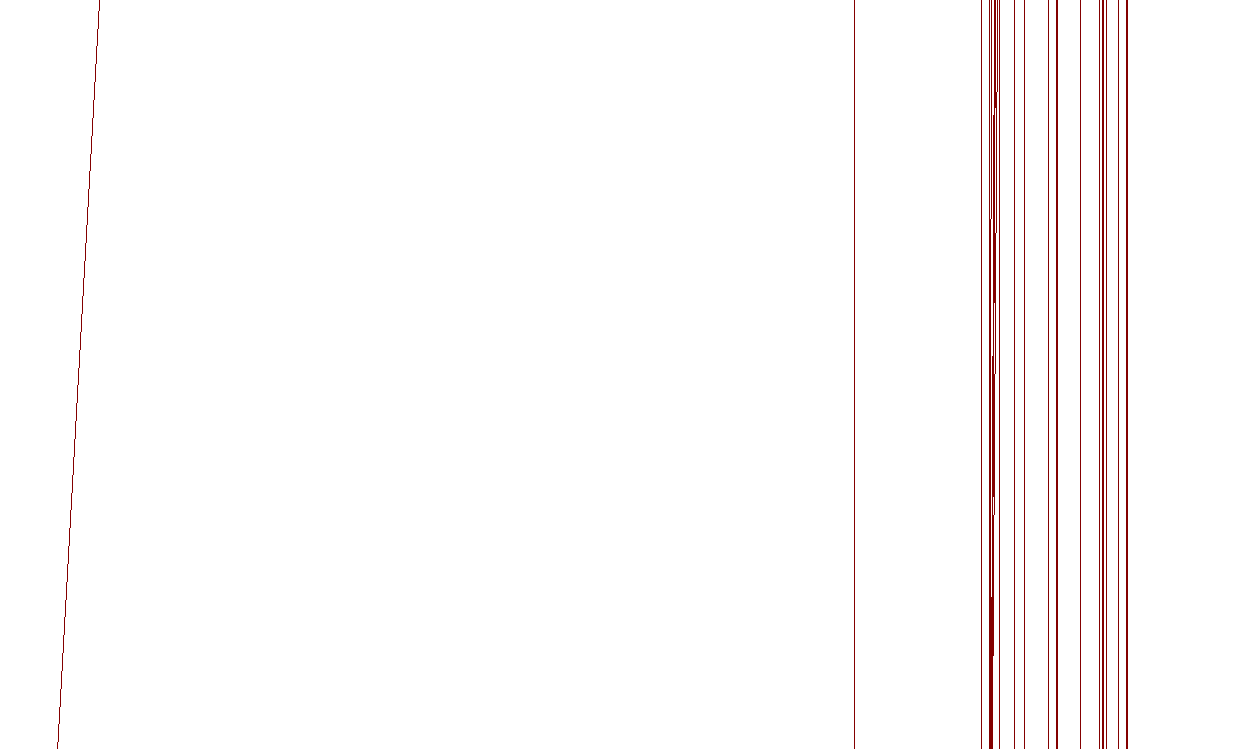
\includegraphics[width=0.95\textheight, angle=90]{obrazky-figures/circuits.pdf}
\end{figure}

%\clearpage
%\thispagestyle{empty}

\begin{figure}[H]
    \centering
    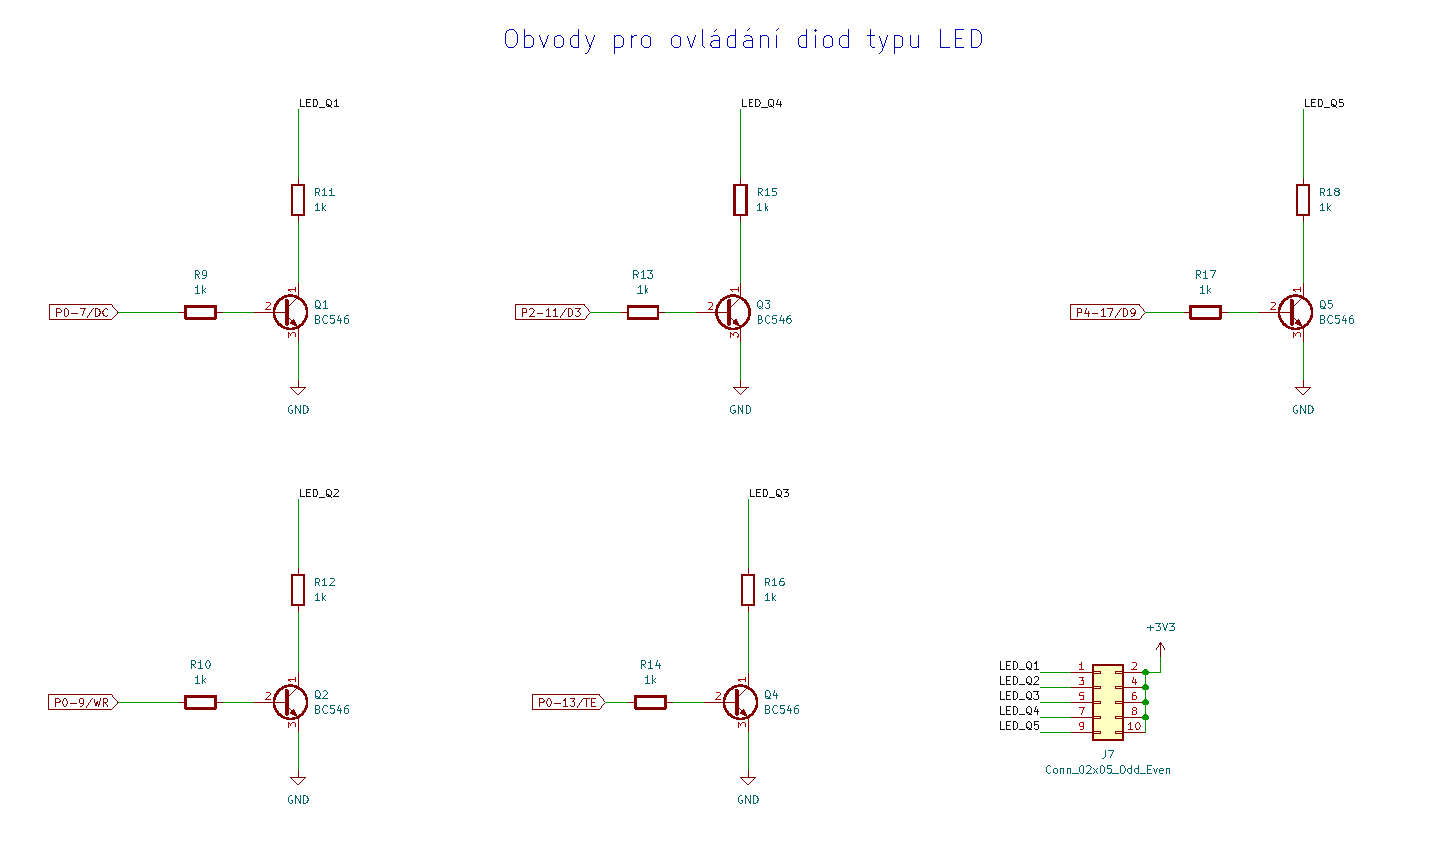
\includegraphics[width=1.00\textheight, angle=90]{obrazky-figures/diodes.pdf}
\end{figure}

%\clearpage
%\thispagestyle{empty}

\begin{figure}[H]
    \centering
    \includegraphics[width=1.00\textheight, angle=90]{obrazky-figures/pin-headers.pdf}
\end{figure}

\chapter{Layout expanzní desky}

\begin{figure}[H]
    \centering
    \includegraphics[width=0.67\textheight, angle=90]{obrazky-figures/extension_shield-brd-front.pdf}
    \caption{Layout expanzní desky -- přední strana}
    \label{fig:layout-front-big}
\end{figure}

\begin{figure}[H]
    \centering
    \includegraphics[width=0.67\textheight, angle=90]{obrazky-figures/extension_shield-brd-back.pdf}
    \caption{Layout expanzní desky -- spodní strana}
    \label{fig:layout-back-big}
\end{figure}

\chapter{Seznam použitých komponent}

\begin{table}[htbp]
    \centering
    \caption{Přehled použitých komponent}
    \label{tab:bom}
    \begin{tabularx}{\textwidth}{|X|X|c|}
        \hline
        \textbf{Komponenta} & \textbf{Hodnota / Popis} & \textbf{Počet} \\
        \hline
        NXP FRDM-MCXN947    & vývojová deska                 & 1  \\ \hline
        SSQ-108-03-T-D      & 16-pinová lišta (Samtec)       & 2  \\ \hline
        SSQ-106-03-T-D      & 12-pinová lišta (Samtec)       & 1  \\ \hline
        SSQ-114-03-T-D      & 28-pinová lišta (Samtec)       & 1  \\ \hline
        SSQ-116-03-T-D      & 32-pinová lišta (Samtec)       & 1  \\ \hline
        SSQ-110-03-T-D      & 20-pinová lišta (Samtec)       & 1  \\ \hline
        M20-7830342         & 10-pinová lišta (Harwin)       & 1  \\ \hline
        DS3231M+            & Obvod reálného času             & 1  \\ \hline
        SCMR14G334SRBB0     & Superkondenzátor (\mbox{KYOCERA AVX})  & 1  \\ \hline
        RSX301L-30DDTE25    & Schottky dioda (ROHM)           & 1  \\ \hline
        BC546               & NPN tranzistor (ON Semi)        & 5  \\ \hline
        Bateriový box CR2032 & --                             & 1  \\ \hline
        THT rezistor        & $\SI{10}{\ohm}$                 & 1  \\ \hline
        SMD rezistor R1206  & $\SI{18}{\kilo\ohm}$            & 1  \\ \hline
        SMD rezistor R1206  & $\SI{33}{\kilo\ohm}$            & 1  \\ \hline
        SMD rezistor R1206  & $\SI{1}{\kilo\ohm}$             & 14 \\ \hline
        SMD kondenzátor R1206  & $\SI{1}{\nano\farad}$        & 1  \\ \hline
    \end{tabularx}
\end{table}

\chapter{Projekt digitálního záznamníku}
Digitální záznamník je možné dále rozšířit nebo upravit dle konkrétních požadavků. Celý projekt, včetně implementace firmwaru, návrhu expanzní desky i veškeré dokumentace, je veřejně dostupný na platformě GitHub.

\begin{itemize}
    \item Odkaz na GitHub repozitář je \url{https://github.com/Doly02/nxp-mcxn947-datalogger}
\end{itemize}
    
\chapter{Použité nástroje}

\begin{itemize}
    \item \textbf{MCUXpresso IDE} ve verzi 11.10.0, jež bylo využito jako hlavní vývojové prostředí pro implementaci firmwaru digitálního záznamníku.
    \item \textbf{NXP SDK FRDM-MCXN947} ve verzi 2.16.000 včetně kterého jsou ovladače pro desku \textbf{FRDM-MCXN947}, knihovna \textbf{FATFS}, operační systém reálného času \textbf{FreeRTOS} a~moduly \textbf{Mass Storage}, \textbf{MMC} a~\textbf{USB}.
    \item \textbf{MCU LinkServer}, který byl použitý pro nahrávání a ladění firmwaru.
    \item \textbf{nRF Connect for Desktop} od \textbf{Nordic Semiconductor} pro měření spotřeby digitálního záznamníku pomocí \textbf{Power Profiler Kit II}.
    \item \textbf{Logic} ve verzi 2.4.22 pro pozorování signálů digitálního záznamníku pomocí logického analyzátoru \textbf{Saleae Logic Pro~16}.
    \item \textbf{GitHub} pro verzování firmwaru digitálního záznamníku a~technické zprávy.
    \item \textbf{KiCAD 8} pro návrh expanzní desky digitálního záznamníku.
    \item \textbf{PC-lint Plus} ve verzi 2.2 pro statickou analýzu zdrojového kódu. 
    \item \textbf{Doxygen} pro generování HTML a~LaTeX dokumentace zdrojového kódu.
    \item \textbf{Overleaf} pro úpravu zdrojových souborů technické zprávy.
    \item \textbf{Draw.io} pro tvorbu diagramů, které jsou součástí technické zprávy.
    \item \textbf{ChatGPT}, který byl využit pro návrhy vylepšení struktury a~formulace vět v~technické zprávě.
\end{itemize}

% Pro kompilaci po částech (viz projekt.tex) nutno odkomentovat
%\end{document}

  \fi
  
  % Kompilace po částech (viz výše, nutno odkomentovat)
  % Compilation piecewise (see above, it is necessary to uncomment it)
  %\subfile{projekt-30-prilohy-appendices}
  
\end{document}
